\documentclass[final]{fhnwreport}       %[mode] = draft or final
                                        %{class} = fhnwreport, article, 
                                        %          report, book, beamer, standalone
%%---Main Packages-----------------------------------------------------------------------
\usepackage[english, ngerman]{babel}	%Mul­tilin­gual sup­port for LaTeX
\usepackage[T1]{fontenc}				%Stan­dard pack­age for se­lect­ing font en­cod­ings
\usepackage[utf8]{inputenc}				%Ac­cept dif­fer­ent in­put en­cod­ings
\usepackage{lmodern}                    %The newer Font-Set
\usepackage{textcomp}					%LaTeX sup­port for the Text Com­pan­ion fonts
\usepackage{caption}					%Customising captions in floating environments
\usepackage{graphicx} 					%En­hanced sup­port for graph­ics
\usepackage{float}						%Im­proved in­ter­face for float­ing ob­jects
\usepackage{ifdraft}                    %Let you check if the doc is in draft mode
\usepackage{wrapfig}                    %Let wrap text around figures

%%---Useful Packages---------------------------------------------------------------------
\usepackage{color}						%Colour control for LaTeX documents
\usepackage[pdftex,dvipsnames]{xcolor}  %Driver-in­de­pen­dent color ex­ten­sions for LaTeX
\usepackage{csquotes}                   %Simpler quoting with \enquote{}
\usepackage{siunitx} 					%A com­pre­hen­sive (SI) units pack­age
\usepackage{listings}					%Type­set source code list­ings us­ing LaTeX
\usepackage[bottom]{footmisc}			%A range of foot­note op­tions
\usepackage{footnote}					%Im­prove on LaTeX's foot­note han­dling
\usepackage{verbatim}					%Reim­ple­men­ta­tion of and ex­ten­sions to LaTeX ver­ba­tim
\usepackage[textsize=footnotesize]{todonotes} %Mark­ing things to do in a LaTeX doc­u­ment
\usepackage{titling}					%Control over the typesetting of the \maketitle command

%%---Tikz Packages-----------------------------------------------------------------------
\usepackage{standalone}
\usepackage{tikz}
\usepackage{circuitikz}
\usetikzlibrary{arrows}
\usetikzlibrary{calc}
\usetikzlibrary{intersections}

%%---Math Packages-----------------------------------------------------------------------
\usepackage{amsmath}					%AMS math­e­mat­i­cal fa­cil­i­ties for LaTeX
\usepackage{amssymb}					%Type­set­ting symbols (AMS style)
%\usepackage{amstext}
%\usepackage{amsfonts}
%\usepackage{breqn}
\usepackage{array}						%Ex­tend­ing the ar­ray and tab­u­lar en­vi­ron­ments
\usepackage{amsthm}					%Type­set­ting the­o­rems (AMS style)

%%---Table Packages----------------------------------------------------------------------
\usepackage{booktabs}
%\usepackage{vcell}
\usepackage{tabularx}					%Tab­u­lars with ad­justable-width columns
%\usepackage{longtable}
\usepackage{multirow}					%Create tab­u­lar cells span­ning mul­ti­ple rows
\usepackage{makecell}
\usepackage{multicol}					%In­ter­mix sin­gle and mul­ti­ple columns
\usepackage[normalem]{ulem}
\useunder{\uline}{\ul}{}

%%---PDF / Figure Packages---------------------------------------------------------------
\usepackage{pdfpages}					%In­clude PDF doc­u­ments in LaTeX
\usepackage{pdflscape}					%Make land­scape pages dis­play as land­scape
\usepackage{subfig}					    %Fig­ures di­vided into sub­fig­ures

%%---Other Packages----------------------------------------------------------------------
%\usepackage{xargs}                     %De­fine com­mands with many op­tional ar­gu­ments

\lstset{
	aboveskip=1ex,
	backgroundcolor=\color{gray!25},
	basicstyle=\small\ttfamily,
	belowskip=1ex,
	breaklines=true,
	columns=fullflexible,
	framerule=0pt,
	framexrightmargin=0em,
	framexleftmargin=0em,
	numbers=left,
	numberstyle=\footnotesize\sffamily,
	tabsize=2
}

\lstdefinestyle{DOS}
{
	backgroundcolor=\color{black},
	basicstyle=\scriptsize\color{white}\ttfamily
}


%%---Bibliography------------------------------------------------------------------------
\usepackage[style=ieee,urldate=comp,backend=biber]{biblatex}
\addbibresource{literature/bibliography.bib}

%%---Main Settings-----------------------------------------------------------------------
\graphicspath{{./graphics/}}			%Defines the graphicspath
\geometry{twoside=false}				    %twoside=false disables the "bookstyle"
\setlength{\marginparwidth}{2cm}
\overfullrule=5em						%Creates a black rule if text goes over the margins => debugging




%%---User Definitions--------------------------------------------------------------------
%%Tabel-Definitions: (requires \usepackage{tabularx})
\newcolumntype{L}[1]{>{\raggedright\arraybackslash}p{#1}}    %column-width and alignment
\newcolumntype{C}[1]{>{\centering\arraybackslash}p{#1}}
\newcolumntype{R}[1]{>{\raggedleft\arraybackslash}p{#1}}

%%---Optional Package Settings-----------------------------------------------------------
%Listings-Settings: (requires \usepackage{listings}) => Example with Matlab Code
%\lstset{language=Matlab,%
%    basicstyle=\footnotesize\ttfamily,
%    breaklines=false,%
%    morekeywords={switch, case, otherwise},
%    keywordstyle=\color{Blue},%
%    tabsize=2,
%    %morekeywords=[2]{1}, keywordstyle=[2]{\color{black}},
%    identifierstyle=\color{Black},%
%    stringstyle=\color{Purple},
%    commentstyle=\color{Green},%
%    showstringspaces=false,%without this there will be a symbol in the places where there is a space
%    numbers=left,%
%    numberstyle={\tiny \color{black}},% size of the numbers
%    numbersep=9pt, % this defines how far the numbers are from the text
%    %emph=[1]{word1, word2,...},emphstyle=[1]\color{red}
%}							

%Hurenkinder und Schusterjungen verhindern (kein Scherz, Google es)
\clubpenalty10000
\widowpenalty10000
\displaywidowpenalty=10000	


%%---Costum Packages Bachelor Thesis-------------------------------------------
\usepackage{diagbox}

\usepackage{hyperref}
\hypersetup{
    colorlinks=true,
    linkcolor=black,
    filecolor=black,       
    urlcolor=blue,
    citecolor=black,
}			                %loads all packages, definitions and settings
\addbibresource{literature/bibliography.bib}							
\title{Testumgebung und Performancevergleich von Zigbee, Thread und Bluetooth Mesh Netzwerken}  		        %Project Title
\author{Anklin, Bobst, Horath}      				    %Document Type => Technical Report, ...
\date{\today}          				   %Place and Date

\setcounter{tocdepth}{2} %%%

\begin{document}

%%---TITLEPAGE---------------------------------------------------------------------------------
\thispagestyle{empty}
%	\ohead{\includegraphics[scale=0.5]{Bilder/Logo_FHNW.jpg}}
	\begin{figure}
		 \vspace*{-\topskip}\vspace*{-\headsep}
		
\includegraphics[scale=1]{graphics/fhnw_ht_logo_de.pdf}
	\end{figure}
	\begin{center}
		\vspace*{2cm}
		{\huge{\textbf{\thetitle}}}\\
		\vspace*{1cm}
		
		{\huge{Bachelor Thesis}}\\
		\vspace*{0.5cm}
		
		{\scshape\Large Fachbericht - \theauthor \\} \Large{\today}
		\vfill
		
		
		\begin{normalsize}
			{\begin{tabbing}
						
					\textbf{Experte:} \hspace{6cm}\= Jürg M. Stettbacher\\					
					\\[0.4cm]
					
					\textbf{Fachcoach:}\>Matthias Meier\\
					\>Manuel Di Cerbo\\
					
					\\[0.4cm]
					
					\textbf{Autoren:} \>Raffael Anklin \\ \>Robin Bobst \\ \>Cyrill Horath
					\\[0.8cm]
					\textbf{Studiengang:} \>Elektro- und Informationstechnik
					\\[0.8cm]	\textbf{Semester:} \>Frühlingssemester 2020
			\end{tabbing}}
		\end{normalsize}
		\vfill
	\end{center}
\clearpage

%%---ABSTRACT----------------------------------------------------------------------------
\selectlanguage{english}				%ngerman or english
\thispagestyle{empty}
\begin{abstract}
	Among the most popular low power mesh network protocols in free GHz ISM band the three mesh stacks Bluetooth Mesh, ZigBee and Thread are currently competing against each other. The assignment of this bachelor thesis was to build a consistent test framework for all three mesh-networks to benchmark them under realistic conditions. Due to better combability\todo{What ist combability? Is this a Robintypo?}, the nRF52840 SoC from Nordic Semiconductors was the chosen microcontroller for all three network stacks. The benchmark is structured in two parts, a battery powered slave node and a master which is directly connected to a computer. The master node is responsible for controlling the measurement, whereas the slave nodes send benchmark messages to each other. These benchmark messages collect the necessary information to determine latency, RSSI, throughput and active radio time. For a better comparability an apartment house, an apartment and a labor environment were selected as different test benches. The Thread stack results the best in the different test benches. Because of its automatic routing it is able to adapt himself to the environment, as a result the latency of this stack is in every three benches similarly low. Bluetooth Mesh was able to reach the lowest latency with small payload. The ZigBee network stands out with its constant and low latency within one test bench. As a conclusion all of the three networks perform well in case of a home automation. Due to of their own assets and drawbacks it cannot be said this is the best mesh-stack. It depends on the application which mesh network performs the best.
\end{abstract}




%%---TABLE OF CONTENTS-------------------------------------------------------------------
\pagenumbering{Roman}		
\selectlanguage{ngerman}				%ngerman or english
\tableofcontents
\clearpage

%%---TEXT--------------------------------------------------------------------------------
\pagenumbering{arabic}

%%Part 0 Allgemeiner Teil

\clearpage

\section{Einleitung}\label{sec:Einleitung}

\todo[inline]{Allgemeine Einleitung in das Thema und die Arbeit. Die Gliederung des Berichts und die Aufteilung in Total 5 Teile soll erläutert werden --> Leseführung.}

\todo[inline]{Cyrill}
\pagebreak

\clearpage

\section{Übersicht}\label{sec:Uebersicht}



\subsection{Ausgangslage und Aufgabenstellung}\label{subsec:AusgangslageundAufgabenstellung}
\todo[inline]{Die Aufgabenstellung soll kurz zusammengefasst werden (komplette Aufgabenstellung im Anhang) und die Ausgangslage abgegrenzt werden.}

\subsection{Vorarbeiten P5}\label{subsec:VorarbeitenP5}
\todo[inline]{Zusammenfassung über die Ergebnisse des P5. Ausserdem Erläuterung "Themenwechsel" zu Thesis (BL Mesh --> 3 Protokolle).}


\subsection{Ziel der Arbeit}\label{subsec:ZielderArbeit}
\todo[inline]{Zusammenfassung der Ziele aus Pflichtenheft (komplettes Pflichtenheft im Anhang). Validierung dieser Ziele erfolgt im Schlussteil dieses Berichts.}









\pagebreak

\vspace*{4cm}
\begin{center}
\part{Point to Point Testinfrastruktur}\label{part:PointtoPointTestinfrastruktur}
\end{center}
\vspace*{\fill}
\clearpage

\section{Messkonzept}\label{sec:KonzeptP2PMessung}
In den nachfolgenden Abschnitten wird auf die Kon­zep­ti­o­nie­rung und Umsetzung der Point to Point (P2P) Testinfrastruktur eingegangen.
Ziel dieser Infrastruktur ist, die Verbindungen auf den MAC-Layern \textit{BLE} sowie \textit{IEEE 802.15.4} auszumessen.
Die Mac-Layer Verbindung beschreibt eine rudimentäre Kommunikation zwischen zwei Knoten, welche direkt auf der physikalischen Schicht stattfindet und keine Netzwerk- und Applikationsschichten daran beteiligt sind.
Dazu wird zuerst das Messkonzept präsentiert und anschliessend die Inbetriebnahme und Bedienung der Messinfrastruktur erläutert. Schliesslich werden noch die technischen Einzelheiten hinsichtlich der Umsetzung dargelegt.

\subsection{Definition MAC-Layer}\label{sec:MAC-LayerP2P}
Der MAC-Layer ist bei Protokollen für die drahtlose Kommunikation oftmals über Normen spezifiziert. Die eingesetzte Hardware-Plattform (siehe Abschnitt \ref{sec:HardwarePlattform}) unterstützt \textit{BLE} sowie den \textit{IEEE 802.15.4} Standard.
Diese beiden Standards werden im Weiteren als Radio-Mode bezeichnet. Nebst dem Radio-Mode charakterisiert sich die MAC-Schicht über den verwendeten Kanal. Dabei handelt es sich um das Frequenzband, auf welchem gesendet wird. 

\subsection{Anforderungen}\label{subsec:AnforderungenP2P}

Die Anforderung an die Point-to-Point Testinfrastruktur ist, eine Verbindung zwischen zwei Funkmodulen anhand der folgenden Messwerte charakterisieren zu können:

\begin{itemize}
	\item \textit{\textbf{Signal to Noise Ratio (SNR)}}
	\item \textit{\textbf{Packetloss}}
\end{itemize}

Das Ausmessen der obigen Eigenschaften soll pro Kanal möglich sein. Die folgenden Parameter müssen vom Benutzer eingestellt werden können, um eine Messung durchzuführen:

\begin{itemize}
	\item \textit{\textbf{Radio-Mode}} BLE-1Mbit oder IEEE 802.15.4
	\item \textit{\textbf{Start-Channel:}} Der Start-Channel definiert den Kanal, auf welchem die Messung gestartet werden soll. Dieser ist abhängig vom Radio-Mode.
	\item \textit{\textbf{Stop-Channel:}} Der Stop-Channel definiert den Kanal, bis zu welchem die Messung durchgeführt werden soll. Dieser ist ebenfalls abhängig vom Radio-Mode.
	\item \textit{\textbf{Tx-Power:}} Sendeleistung beim Versand der Testnachrichten.
	\item \textit{\textbf{Collision-Avoidance (CA):}} Kollisionsvermeidung (nur bei IEEE 802.15.4 Radio Mode)
	\item \textit{\textbf{Payload:}} Anzahl der zu sendenden Bytes pro Paket.
\end{itemize}


\subsection{Messgrössen}\label{subsec:MessgrössenP2P}
Wie bereits in Abschnitt \ref{subsec:AnforderungenP2P} erwähnt, wird das Signal-Rausch-Verhältnis (SNR) und der Paketverlust gemessen. Die beiden Messgrössen können mit Hilfe der nRF-Plattform direkt bestimmt werden.

\begin{itemize}
	\item \textbf{\textit{SNR}}: Gibt das Verhältnis zwischen der Signalleistung und Rauschleistung an. Als Rauschen werden jegliche Umwelteinflüsse (Störungen) bezeichnet. Zur Bestimmung des SNR muss die Rauschleistung und Signalleistung erfasst werden.
	Bei der Detektion der Rauschleistung muss der Signalbringer (Sender) deaktiviert sein. Das Messen der Signalleistung inkl. Rauschleistung erfolgt hingegen bei eingeschaltetem Sender.
	
	\item \textbf{\textit{Paketverlust}}: Als Paketverlust wird das Verhältnis zwischen der Anzahl Pakete bezeichnet, die das Ziel nicht erreicht haben, zu der totalen Anzahl versendeten Pakete.
	Zur Bestimmung dieses Verhältnisses werden Pakete generiert und vom Sender zum Empfänger übermittelt. Dieser zählt die Anzahl empfangener Pakete und meldet den Zählwert dem Sender zurück. Damit ist der Sender in der Lage, den Paketverlust zu berechnen. 
\end{itemize} 


\subsection{Konzept}\label{sec:KonzeptP2P}
Zur Realisierung der Point to Point Testinfrastruktur wurde auf ein \textit{One to Many} (1:n) Messprinzip gesetzt (auch als Multicast bezeichnet). Dies hat den Vorteil, dass mehrere Verbindungen gleichzeitig ausgemessen werden können. Der Nachteil dabei ist, dass so die Messpfade nur unidirektional charakterisiert werden (nur von Master zu Slave oder Uplink-Pfad). Die Abweichung zwischen Up- und Downlink Pfad kann durch die Wiederholung der Messung mit vertauschten Standorten verifiziert werden. 

\begin{figure} [H]
	\centering
	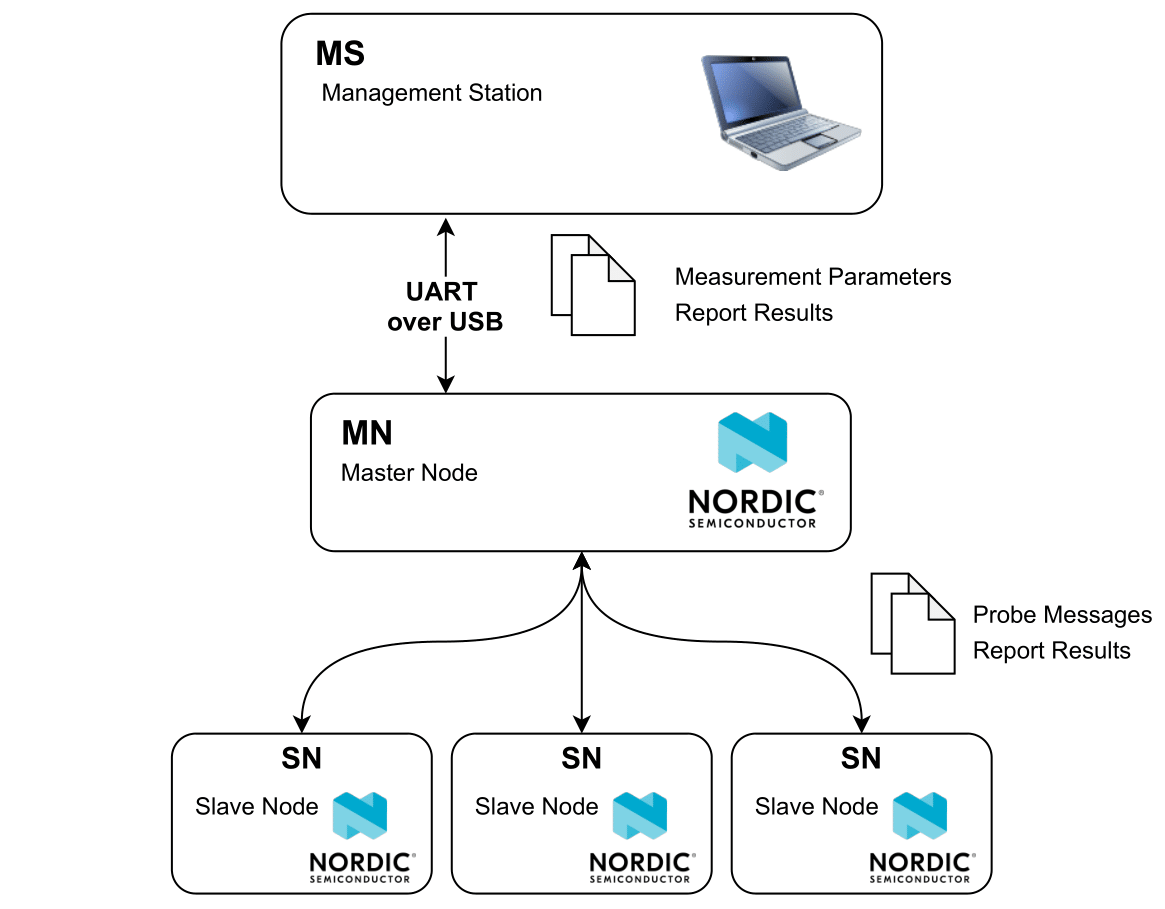
\includegraphics[width=0.7\textwidth]{Konzeptschema_P2P.png}
	\caption{Konzeptschema P2P Testinfrastruktur}
	\label{fig:KonzeptschemaP2P}
\end{figure}

\todo[inline]{Cyrill: Grafik korrigieren}


Das in Abbildung \ref{fig:KonzeptschemaP2P} gezeigte Konzept besteht aus einer Management Station, einem Master- und mehreren Slave Nodes.
Über die Management Station können Messresultate angezeigt sowie Messparameter eingestellt werden. Als Ausgangspunkt zur Messung dient der MN (Master Node).
Er koordiniert den Messablauf und sendet \textit{Probe Packets} an alle SN (Slave Nodes).
Diese protokollieren die Anzahl empfangener \textit{Probe Packets} und melden ihre Messresultate an den MN zurück.
Nach Empfang aller Resultate leitet der MN alle Messergebnisse an die MS weiter.
Dort werden dem Benutzer die Messdaten dargestellt.
Details zum Ablauf sind in Abschnitt \ref{sec:SoftundFirmware} aufgeführt.
Eine mögliche Anwendung der Testinfrastruktur wird im nachfolgenden Abschnitt \ref{sec:TestszenarienP2P} beschrieben.  

\subsection{Testszenarien}\label{sec:TestszenarienP2P}
Die P2P Testinfrastruktur ist als einfach zu bedienendes Tool konzipiert.
Es kann eingesetzt werden, um den Aufbau von sogenannten \textit{Wireless Personal Area Networks (WPAN)} zu optimieren.
Mithilfe dieses Tools können zum Beispiel die Standorte der Teilnehmer eines Zigbee, Thread oder Bluetooth Mesh Netzwerks optimal gewählt werden.

Weiter kann die Testinfrastruktur als Störquelle in den Benchmarks von Mesh Netzwerken eingesetzt werden (siehe Abschnitt \ref{sec:BenchmarkKonzeptMeshNetzwerke}).
Die Form der Störung kann dabei gemäss den einstellbaren Parametern aus Abschnitt \ref{subsec:AnforderungenP2P} frei gewählt werden.

\subsection{Messaufbau}\label{sec:Messaufbau}
Bei der verwendeten Hardware handelt es sich um einen nRF52840 Mikrocontroller (siehe auch Abschnitt \ref{sec:HardwarePlattform}).
Als Master dient das Development-Kit (DK), welches über eine USB-Buchse verfügt.
Als Slaves kommen sowohl DKs als auch die USB-Dongle Variante in Frage.
Letztere sind einfacher unterzubringen und werden in diesem Messaufbau bevorzugt.
Um die erhaltenen Daten auswerten zu können, geschieht die Visualisierung mittels einem Laptop oder PC.
Dieser muss mit der USB Buchse des Masters verbunden werden und die entsprechende Auswertesoftware gestartet sein.
Im nachfolgenden Abschnitt \ref{sec:InbetriebnahmeBedienungP2P} wird die Inbetriebnahme und die Bedienung der P2P-Testinfrastruktur genauer beschrieben.
Die Abbildung \ref{fig:MessaufbauP2P} zeigt den schematischen Messaufbau der P2P-Testinfrastruktur. Der Master kann durch den Einsatz eines Notebooks mobil gehalten werden, um so den optimalen Standort des Masters auszuloten.
Die Slaves werden in der Wohnung oder im Haus an den möglichen Standorten der Mesh Nodes platziert. Danach wird die Messung gestartet.

\begin{figure} [H]
	\centering
	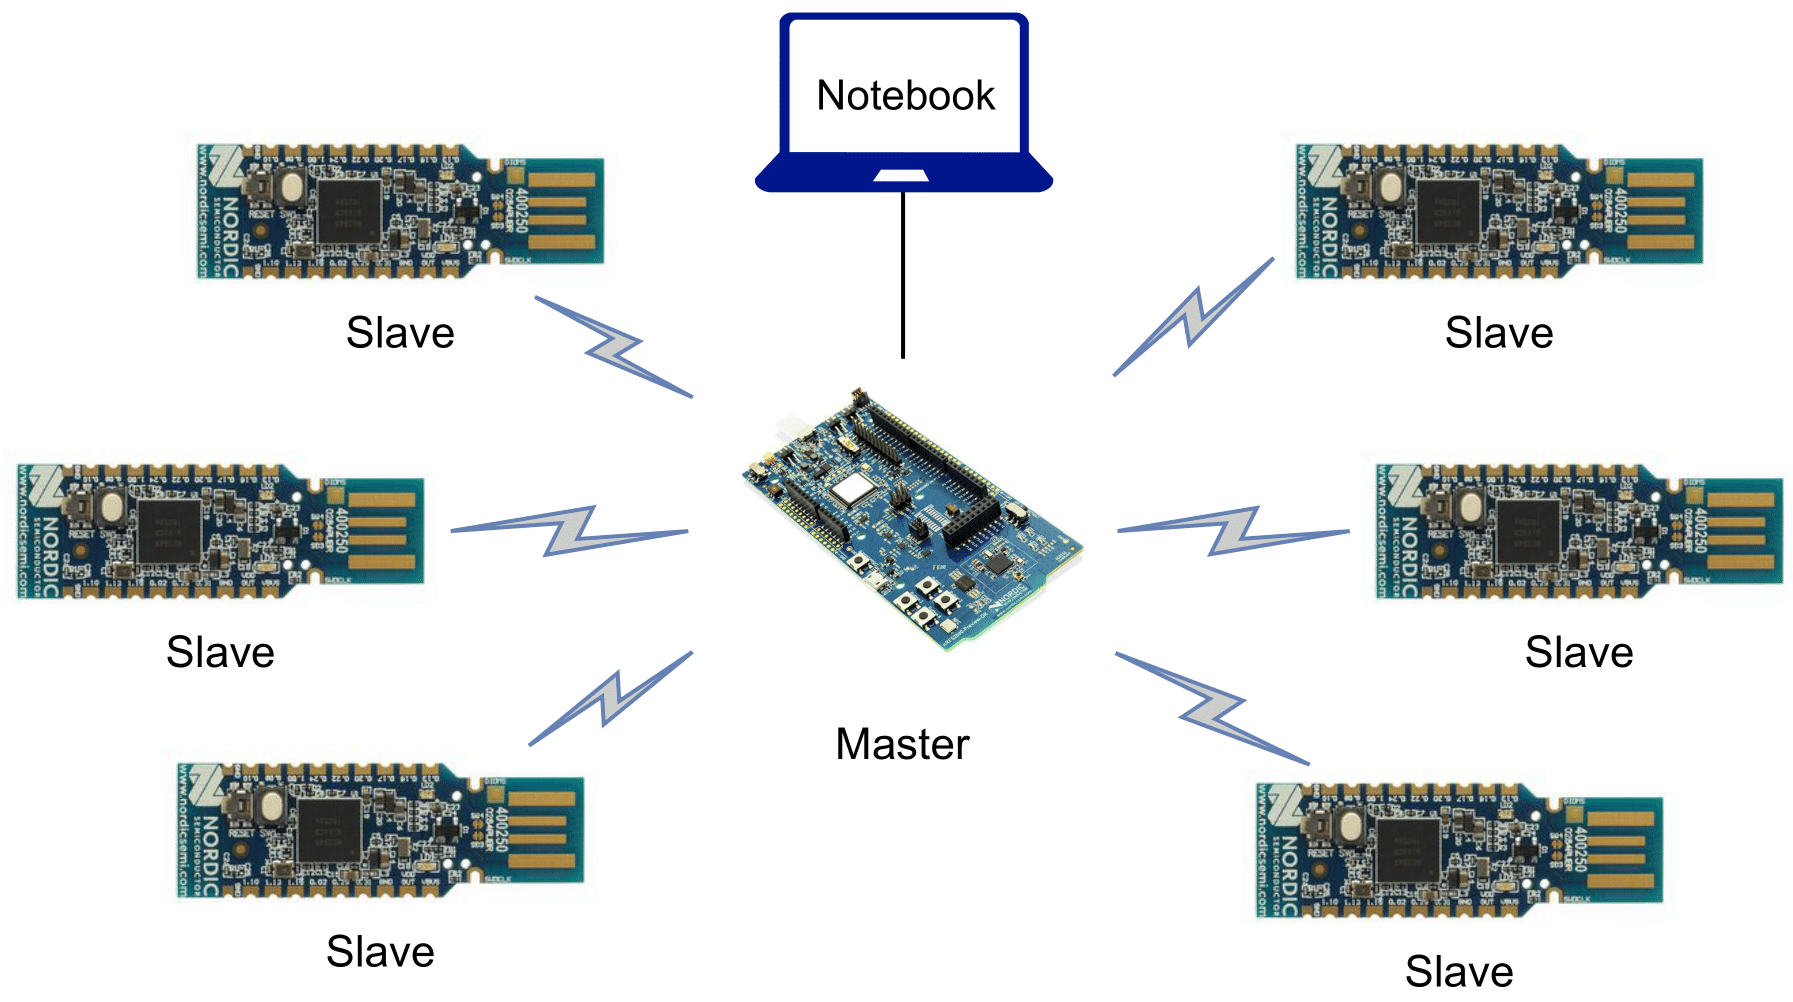
\includegraphics[width=0.8\textwidth]{Messaufbau_P2P.png}
	\caption{Messaufbau P2P Testinfrastruktur}
	\label{fig:MessaufbauP2P}
\end{figure}


\newpage
\section{Inbetriebnahme und Bedienung}\label{sec:InbetriebnahmeBedienungP2P}
Die P2P Testinfrastruktur kann von jedem interessierten Anwender eingesetzt werden.
Zur Inbetriebnahme müssen jedoch folgende Hard- und Software Komponenten vorhanden und einsatzbereit sein: 

\begin{itemize}
	\item 1x nRF52840 DK (Master)
	\item 1x nRF52840 DK / Dongle (Slave)
	\item Laptop mit folgender Software:
	\begin{itemize}
		\item Python 3.x
		\item nrfutil (pip install nrfutil), zum Flashen der nRF52840.
		\item Browser, zur Darstellung der Weboberfläche
	\end{itemize}
\end{itemize}

Eine Anleitung und der Sourcecode sind im \href{https://github.com/Rouben94/P6_Software}{Github-Repository\footnote{\url{https://github.com/Rouben94/P6_Software}\cite{github_p6_software_p2p_2020}}} zu diesem Projekt verfügbar.
Master und Slaves sind mit der entsprechenden Firmware zu laden um diese für die Messung vorzubereiten.
Anschliessend werden die Slaves im Raum platziert und der Master am Laptop eingesteckt.
Nach erfolgtem Setup ist gemäss den nachfolgend beschriebenen Schritten vorzugehen.

\paragraph{Schritt 1 - Webserver Starten}
Der Webserver wurde mit einer Windows Umgebung entwickelt und getestet. Die folgende Anleitung ist demzufolge nur für eine Windows Umgebung gültig.
Für die Verwendung mit Linux oder MacOS sind unter folgendem \href{https://tutorial.djangogirls.org/en/django_installation}{Link\footnote{\url{https://tutorial.djangogirls.org/en/django_installation/}}} entsprechende Anleitungen verfügbar.
Bevor der Webserver gestartet werden kann, muss der Sourcecode vom \href{https://github.com/Rouben94/P6_Software}{Github-Repository\footnotemark[1]} geklont werden.
Auf der Ordnerebene \textbf{P6\_Software\textbackslash P2P\textbackslash Webserver\textbackslash p2p\_webserver} müssen folgende cmd Befehle ausgeführt werden.

\begin{lstlisting}[style=DOS]
Microsoft Windows [Version 10.0.18363.1016]
(c) 2019 Microsoft Corporation. Alle Rechte vorbehalten.

C:\Users\GitHub\P6_Software\P2P\Webserver\p2p_webserver> .\myvenv\Scripts\activate
(myvenv) C:\Users\GitHub\P6_Software\P2P\Webserver\p2p_webserver> python .\manage.py runserver
Performing system checks...
	
System check identified no issues (0 silenced).
August 20, 2020 - 22:01:13
Django version 3.0.8, using settings 'p2p_site.settings'
Starting development server at http://127.0.0.1:8000/   
Quit the server with CTRL-BREAK.
\end{lstlisting}


Sobald dies erfolgreich ausgeführt wurde, ist der Webserver gestartet und kann unter der Adresse \textbf{http://127.0.0.1:8000/} erreicht werden.

\newpage
Falls das Starten nicht geklappt hat, müssen möglicherweise Django und die benötigten Python Bibliotheken nachinstalliert werden. Dies wird wie folgt gemacht:

\begin{lstlisting}[style=DOS]
Microsoft Windows [Version 10.0.18363.1016]
(c) 2019 Microsoft Corporation. Alle Rechte vorbehalten.

C:\Users\GitHub\P6_Software\P2P\Webserver\p2p_webserver> .\myvenv\Scripts\activate
(myvenv) C:\Users\GitHub\P6_Software\P2P\Webserver\p2p_webserver> pip install Django==3.1
(myvenv) C:\Users\GitHub\P6_Software\P2P\Webserver\p2p_webserver> pip install pyserial
(myvenv) C:\Users\GitHub\P6_Software\P2P\Webserver\p2p_webserver> pip install plotly
(myvenv) C:\Users\GitHub\P6_Software\P2P\Webserver\p2p_webserver> python manage.py makemigrations p2p
(myvenv) C:\Users\GitHub\P6_Software\P2P\Webserver\p2p_webserver> python manage.py migrate p2p
(myvenv) C:\Users\GitHub\P6_Software\P2P\Webserver\p2p_webserver> python .\manage.py runserver
Performing system checks...

System check identified no issues (0 silenced).
August 20, 2020 - 22:01:13
Django version 3.0.8, using settings 'p2p_site.settings'
Starting development server at http://127.0.0.1:8000/   
Quit the server with CTRL-BREAK.
\end{lstlisting}

\paragraph{Schritt 2 - Verbindungsaufbau}
Sobald der Webserver gestartet wurde, ist die Seite \textbf{Point to Point} zu sehen (siehe Abbildung \ref{fig:WebserverNodelistViewausgeklappt}). Wie in der Abbildung beschrieben, muss nun auf die Seite Connection gewechselt werden, damit die Verbindung zum Master aufgenommen werden kann. Es besteht die Möglichkeit das Hauptmenü auf der linken Seite auf und zu zuklappen (siehe Nummer 1 in Abbildung \ref{fig:WebserverNodelistViewausgeklappt}). Wenn das Hauptmenü aufgeklappt ist, kann das Github-Repository durch einen Klick auf die Schaltfläche \textbf{GitHub Repo} erreicht werden.
\begin{figure} [H]
	\centering
	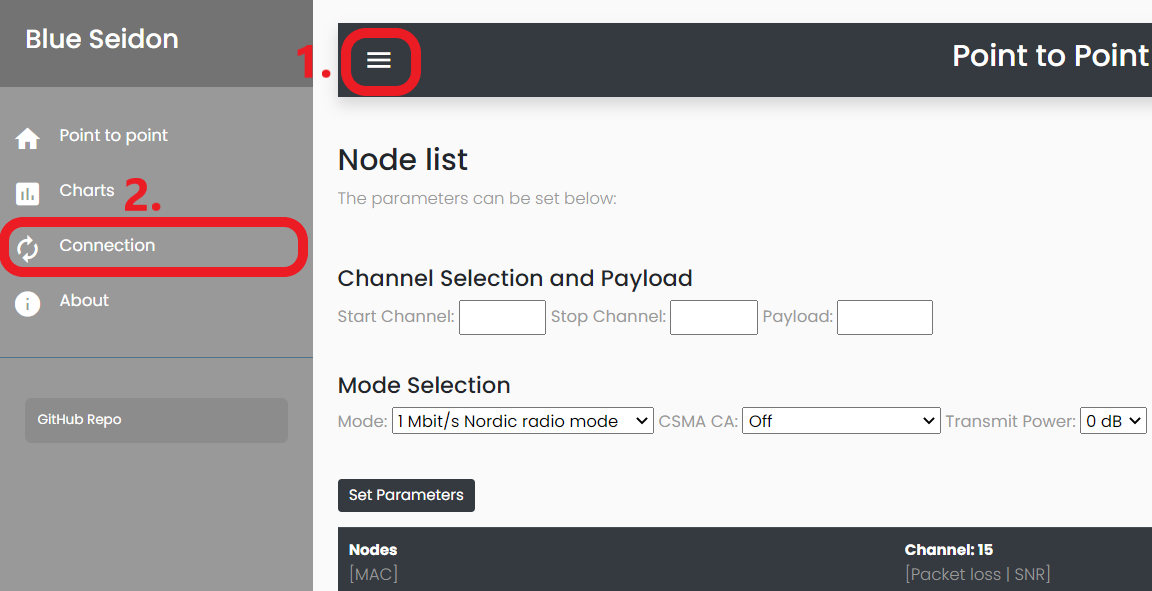
\includegraphics[width=\textwidth]{Webserver_nodelist_ausgeklappt.png}
	\caption{Webserver Nodelist View ausgeklappt}
	\label{fig:WebserverNodelistViewausgeklappt}
\end{figure}

\newpage
Auf der Seite \textbf{Connection} (siehe Abbildung \ref{fig:WebserverConnectionView}) soll für die Kommunikation mit der Seriellen Schnittstelle der entsprechende COM-Port, an dem der Master registriert ist, ausgewählt werden (siehe Nummer 1 in Abbildung \ref{fig:WebserverConnectionView}). Mit einem Klick auf das Feld \textbf{Connect} wird nun eine Verbindung hergestellt (siehe Nummer 2 in Abbildung \ref{fig:WebserverConnectionView}). Falls der Master nicht angeschlossen oder auf einem anderen COM-Port registriert ist, wird dies mit einer Fehlermeldung mitgeteilt.
\begin{figure} [H]
	\centering
	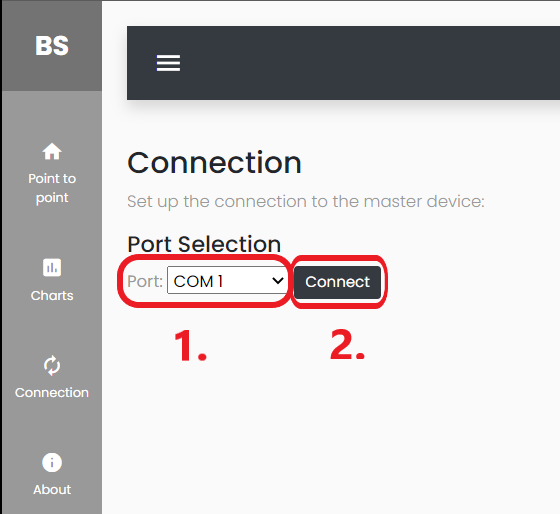
\includegraphics[width=0.6\textwidth]{Webserver_Connection.png}
	\caption{Webserver Connection View}
	\label{fig:WebserverConnectionView}
\end{figure}

\paragraph{Schritt 3 - Einstellen der Parameter}
Nachdem die Serielle Verbindung zum Master hergestellt ist, werden auf der Seite \textbf{Point to Point} die verfügbaren Slaves in der Tabelle aufgeführt. Die Tabelle aktualisiert sich automatisch. Wie in der Abbildung \ref{fig:WebserverNodelistView} ersichtlich, sind die Nodes anhand der MAC-Adresse identifizierbar. Die Tabelle zeigt die dazugehörigen Channels, welche zuvor eingestellt wurden. Pro Channel ist ein Wert für den Packetloss und den SNR zu sehen. Die Definition dieser Werte ist im Kapitel \ref{sec:MessgrössenP2P} beschrieben. 

Damit die Parameter der Nodes verändert werden können, besteht auf der gleichen Seite die Möglichkeit, die gewünschten Werte einzugeben und an den Master zu senden. Die Parameter können, wie in Abbildung \ref{fig:WebserverNodelistView} markiert, definiert werden. Folgende Vorgaben müssen bei der Eingabe eingehalten werden:

\begin{table}[h]
\centering
\begin{tabular}{|l|c|c|} 
\hline
\textbf{Radio Mode} & \textbf{IEEE 802.15.4 250 kBit}  & \textbf{Alle Anderen Modi}  \\ 
\hline
\textbf{Start Channel Feld} & 11 & 0 \\ 
\hline
\textbf{Stop Channel Feld} & 26 & 39 \\ 
\hline
\textbf{Payload Feld} & 0 - 120 bit & 0 - 250 bit \\
\hline
\end{tabular}
\caption{Zulässige Parameter für die Eingabefelder in der Nodelist View}
\label{tab:ParameterEingabefelederNodelistView}
\end{table}


\begin{figure} [H]
	\centering
	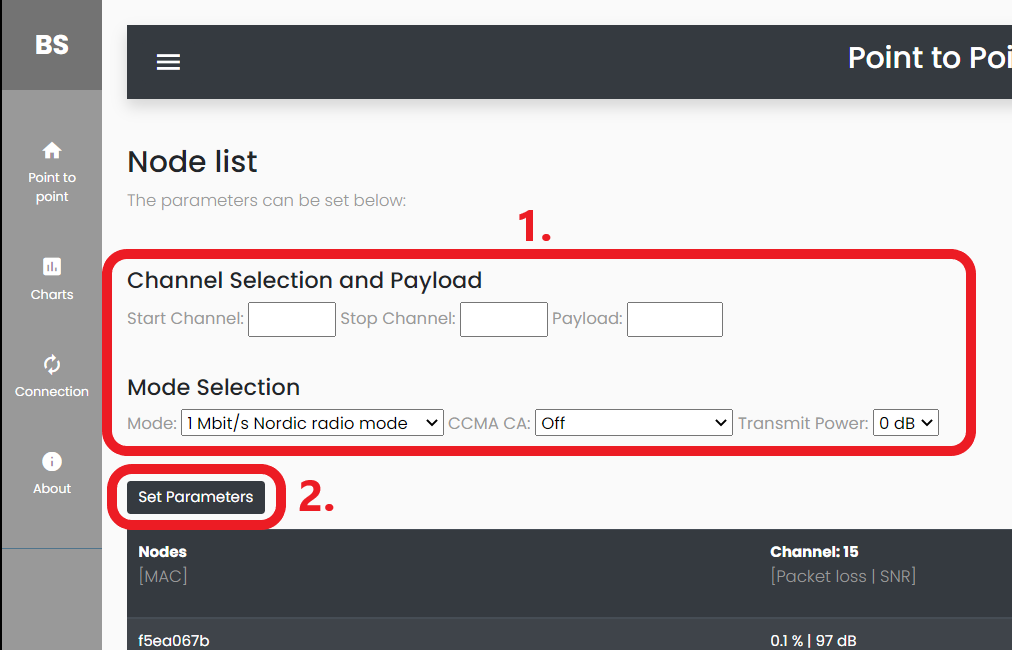
\includegraphics[width=\textwidth]{Webserver_Nodelist.png}
	\caption{Webserver Nodelist View}
	\label{fig:WebserverNodelistView}
\end{figure}

\paragraph{Schritt 4 - Vergleich der Channels}
Damit die Channels von einem Node besser miteinander verglichen werden können, ist auf der Seite Chart eine entsprechende Grafik verfügbar. Jeder Node wird in einem separaten aufklappbaren Fenster angezeigt. In Abbildung \ref{fig:WebserverChartView} mit der Nummer \textbf{1.} gekennzeichnet, ist ein solches Fenster zu sehen. Mit Klick auf die Schaltfläche mit der Nummer \textbf{1.} wird das Fenster aufgeklappt und alle eingestellten Channels werden nacheinander mit dem Packetloss in \% aufgelistet.
\begin{figure} [H]
	\centering
	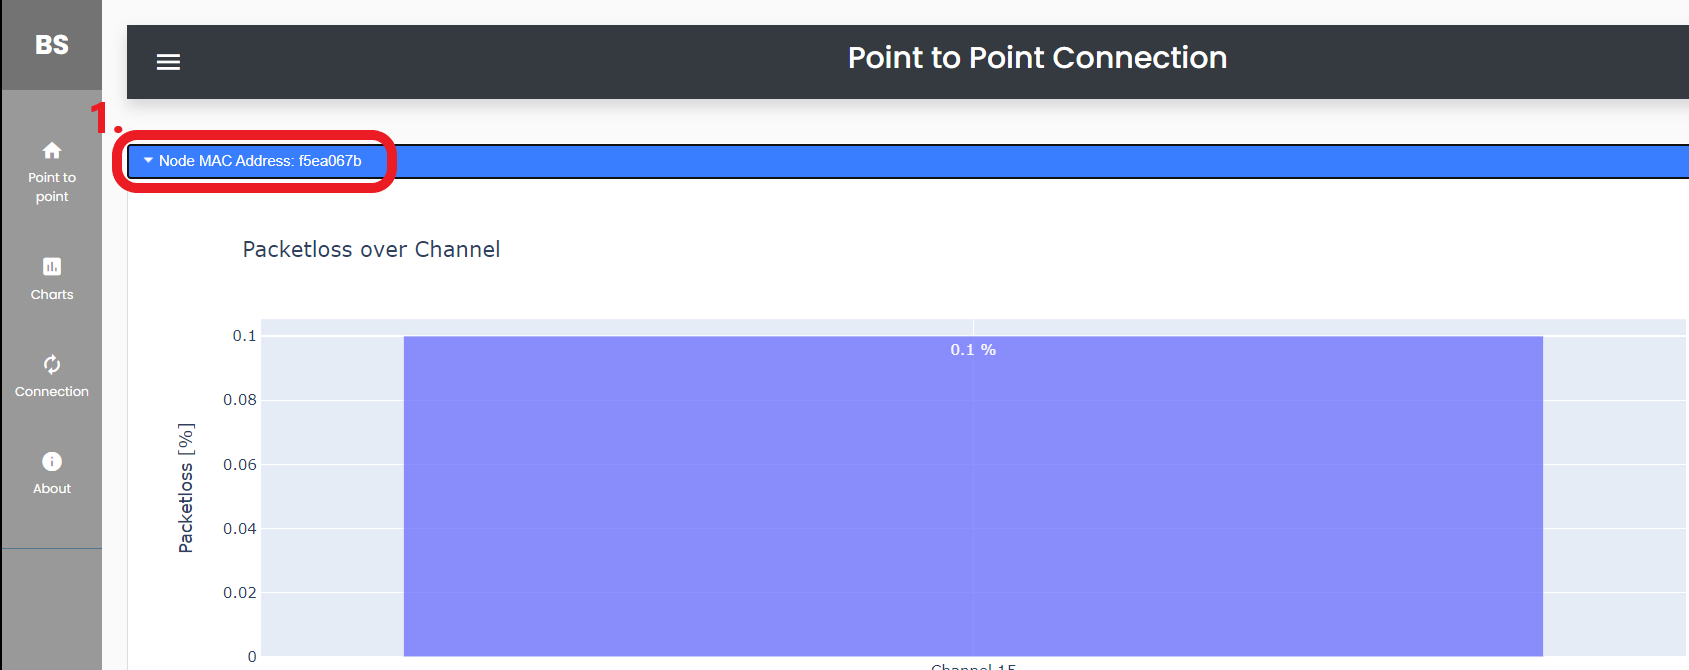
\includegraphics[width=\textwidth]{Webserver_Chart.png}
	\caption{Webserver Chart View}
	\label{fig:WebserverChartView}
\end{figure}

\newpage
\section{Soft- und Firmware}\label{sec:P2PSoft-undFirmware}
In den nachfolgenden Abschnitten wird die Soft- und Firmware für die P2P Testinfrastruktur beschrieben.
Der dazugehörige Sourcecode ist im \href{https://github.com/Rouben94/P6_Software}{Github-Repository\footnote{\url{https://github.com/Rouben94/P6_Software}\cite{github_p6_software_p2p_2020}}} zu diesem Projekt frei zugänglich und kann für die vertiefte Untersuchung konsultiert werden.

\subsection{Soft- und Firmware}\label{sec:SoftundFirmware}
Die Firmware ist als zeitabhängige Schrittkette aufgebaut.
Jeder Schritt ist über ein fixes Zeitfenster definiert.
Damit alle Teilnehmer synchron die Schrittkette abarbeiten können, muss mit Hilfe einer Zeitsynchronisation auf den Master der exakte Startzeitpunkt kommuniziert werden.
Unabhängig vom Zustand des aktiven Schrittes darf dieser sein Zeitfenster nicht überschreiten, ansonsten fällt die Schrittkette aus dem Takt. 

\begin{figure} [H]
	\centering
	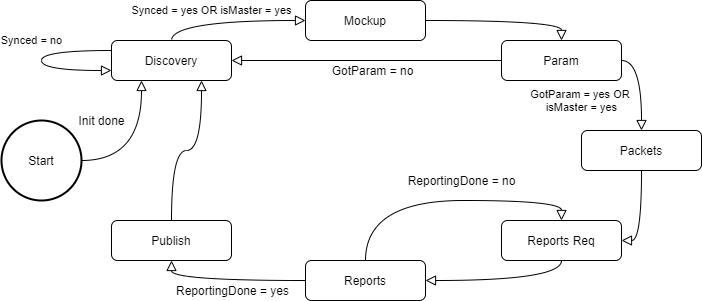
\includegraphics[width=1.0\textwidth]{Software_Flowgraph_P2P.png}
	\caption{Schrittkette P2P Testinfrastruktur}
	\label{fig:FlowgraphP2P}
\end{figure}

Abbildung \ref{fig:FlowgraphP2P} zeigt die Schrittkette für den Master, sowie für die Slave-Nodes.
Der Ablauf zeigt die Schritte, sowie die Bedingungen der Transitionen zwischen den Schritten.
Jedoch muss beachtet werden, dass jeder Schritt immer während einer bestimmten Zeit aktiv bleibt.
Somit ist ersichtlich dass der \textit{Packets-State} nach Ablauf seines Zeitfensters immer zum \textit{ReportsReq-State} führt.
Dabei hängt der Wechsel nach dem \textit{Discovery-State} von verschiedenen Bedingungen ab.

Auf die Funktion der Schritte wird nachfolgend kurz eingegangen: 

\begin{itemize}
	\item \textbf{\textit{Discovery:}} Der Master verteilt die Zeitsynchronisation an die Slaves. Die Slaves synchronisieren sich auf das Signal des Masters auf, sofern sie in seiner Reichweite liegen. Hat ein Slave sich nicht synchronisieren können, verweilt dieser im \textit{Discovery-State}. Der Master kann in jedem Fall zum nächsten Schritt voranschreiten.
	 
	\item \textbf{\textit{Mockup:}} Der Master wartet auf eine Antwort der einzelnen Slaves. Jeder Slave generiert einen zufälligen Timeslot, um sich beim Master anzumelden. Der Master führt alle Slaves, die sich gemeldet haben, in einer Liste auf. Hat sich kein Slave gemeldet, ist diese Liste leer und der Master wird zum \textit{Discovery State} zurückkehren. Ist ein Slave bereits beim Master angemeldet, so muss er sich nicht erneut anmelden. 
	
	\item \textbf{\textit{Param:}} Der Master versendet die Packets-Parameter (Mode, StartChannel, StopChannel, etc.). Erhält ein Slave keine Daten, so kehrt er in den \textit{Discovery-State} zurück. 
	
	\item \textbf{\textit{Packets:}} Der Master versendet \textit{Probe Packets} mit den zuvor kommunizierten Einstellungen. Die Slaves empfangen diese Daten, zählen die Anzahl erfolgreich empfangener Pakete und erfassen weitere Messdaten. 
	\item  \textbf{\textit{Reports Req:}} Nach dem Ausmessen beginnt der Master mit dem Einsammeln der einzelnen Slave Reports. Dazu sendet er an jeden Slave in seiner Liste (aus dem \textit{Mockup-State}) Report-Anfragen, sogenannte \textit{Report-Requests}. Die Slaves warten auf einen \textit{Report Request} vom Master. 
	
	\item  \textbf{\textit{Reports:}} Der Slave, welcher den Request erhalten hat, sendet seinen Report zum Master. Dies hat innerhalb einer gewissen Zeit zu erfolgen. Sendet ein Slave nach einer gewissen Anzahl von Versuchen innerhalb dieser begrenzten Zeit keine Reports, so wird er aus der Liste der gemeldeten Slaves entfernt. Sobald der Master alle Reports von allen Slaves empfangen hat, meldet er an alle Slaves über eine spezielle \textit{Reports-Request-Message}, dass das Reporting beendet ist.
	
	\item  \textbf{\textit{Publish:}} Im \textit{Publishing-State} hat der Master Zeit, die Daten an die übergeordnete Stelle zu übermitteln (USB-UART). Die Slaves können in diesem State Energie sparen. Alle Teilnehmer beginnen wieder von vorne, im \textit{Discovery-State}, wo sie sich neu synchronisieren. 
\end{itemize}


\subsection{Low Level Radio Driver}\label{sec:LowLevelRadioDriver}

Die Kommunikation über das Radio-Interface wurde mittels einem eigens entwickelten Radio-Driver speziell für die nRF52 / nRF53 SOCs ermöglicht. Dieser stellt die nötigen Funktionen für die P2P Testinfrastruktur zur Verfügung. Zum Beispiel kann die Mode- und Kanalwahl sowie das Senden und Empfangen von Daten mittels simplen Kommandos erfolgen. Bei der Entwicklung diente das \textit{Radio Test Example} \cite{nrf_connect_sdk_radio_test_example_2020} als Vorlage. Der Radio-Driver steuert mithilfe der \textit{NRF-HAL Radio Library} oder über direkten Zugriff auf die Peripherie-Register das Radio-Interface an.

\begin{figure} [H]
	\centering
	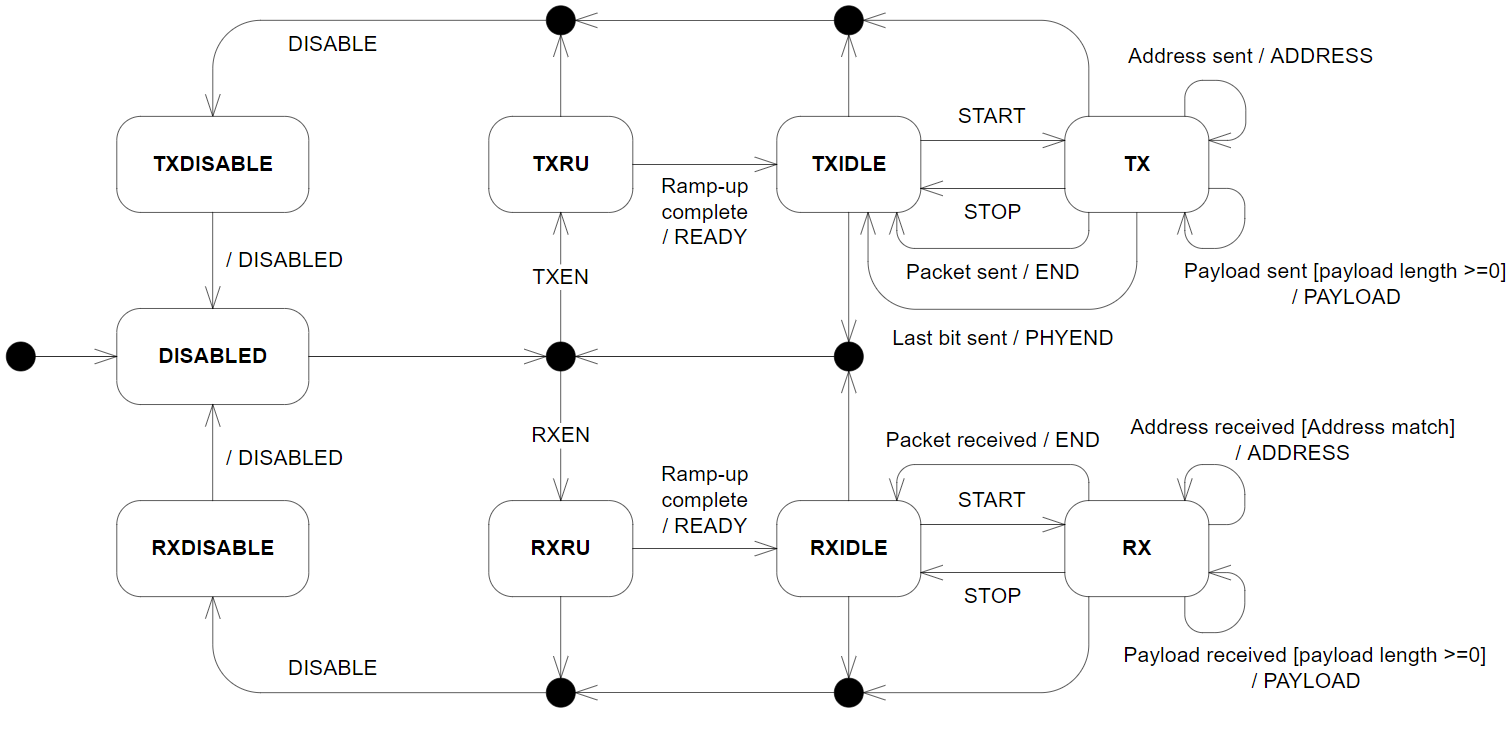
\includegraphics[width=1.0\textwidth]{nRF52840_Radio_states.png}
	\caption{Radio States \cite{nordic_semi_nrf_infocenter_radio_states_2020}}
	\label{fig:RadioStatesP2P}
\end{figure}

Die Radio Hardware der nRF52 und nRF53 SoCs verfügt über verschiedene Zustände (siehe Abbildung \ref{fig:RadioStatesP2P}). Abhängig von der gewünschten Operation (Senden oder Empfangen) werden die States abgearbeitet.
Um Energie zu sparen, wird nach Abschluss der gewünschten Tätigkeit immer in den Disabled-State gewechselt.
Die Benachrichtigung des Radio Drivers durch die Hardware erfolgt zudem mittels Interrupts, wodurch der Energieverbrauch zusätzlich minimiert werden kann.

\begin{figure} [H]
	\centering
	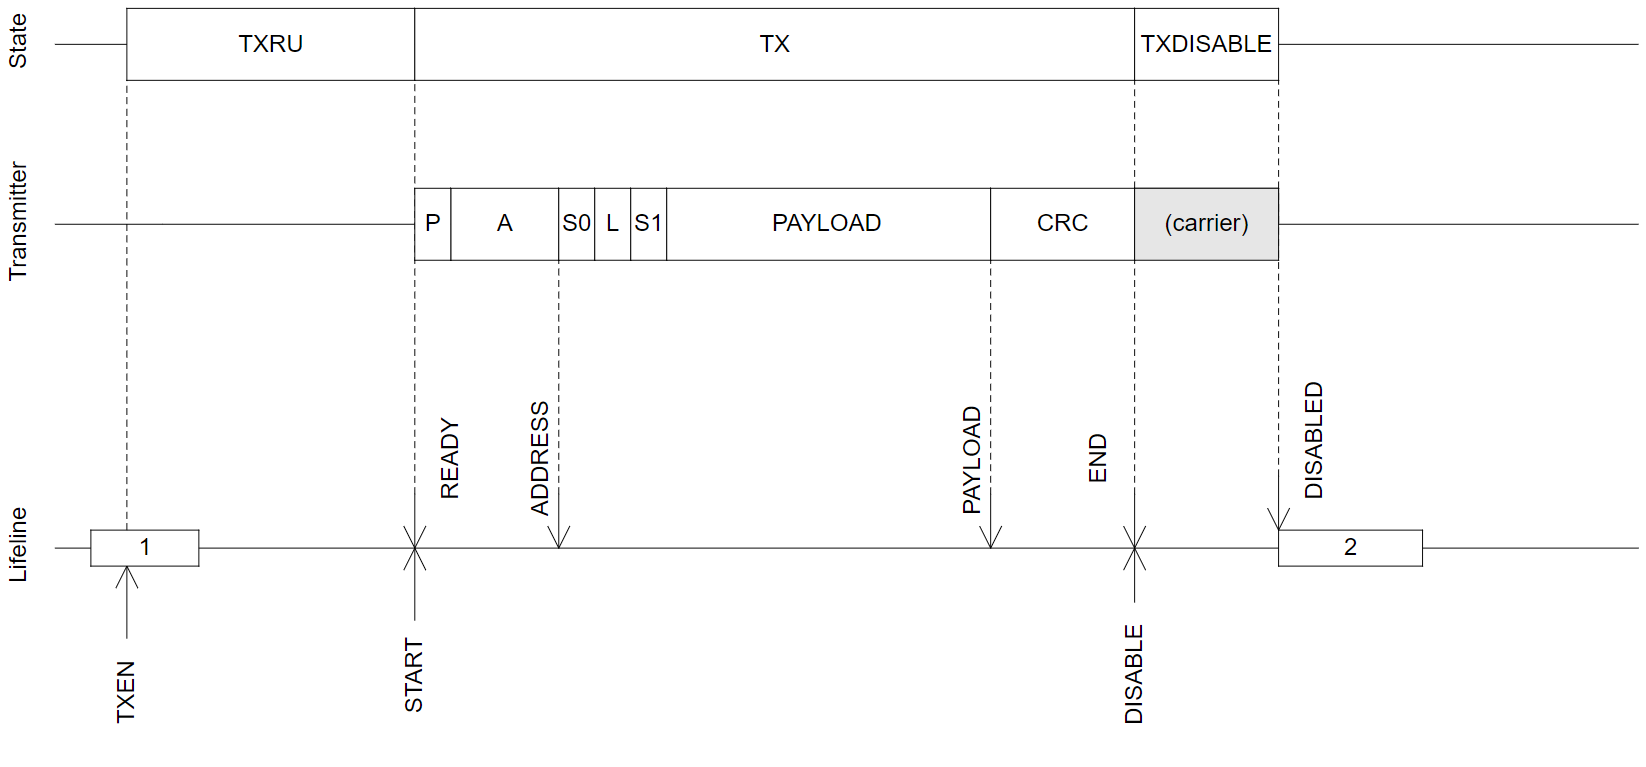
\includegraphics[width=1.0\textwidth]{nRF52840_Radio_Transmit_Sequence_with_Shorts.png}
	\caption{Sende-Ablauf mit Verknüpfungen \cite{nordic_semi_nrf_infocenter_radio_transmit_sequence_2020}}
	\label{fig:RadioTransmitSequP2P}
\end{figure}

Abbildung \ref{fig:RadioTransmitSequP2P} zeigt den Ablauf beim Senden eines Pakets. Die zu sendenden Daten (Payload) müssen vorgängig im RAM vorliegen.
Anschliessend wird der Packet Pointer des Radio-Interface auf die entsprechende Speicher-Adresse eingestellt.
Zu beachten gilt, dass im ersten Byte die Länge der Payload angegeben werden muss.
Diese\todo{Was ist mit DIESE gemeint?} wird vom Radio Driver automatisch ergänzt.
Zusätzlich kann den Sendedaten ein Adressfeld mitgegeben werden. Nach der vollständigen Konfiguration des Radio-Interface wird das Senden durch den Befehl TXEN initiiert. Mithilfe von Verknüpfungen (Shorts) wird nach dem Ready-Event automatisch der Start-Task ausgelöst.
Das Senden läuft also nach dem Initiieren vollautomatisch ab.
Der Radio-Driver wartet auf das Auslösen des Disabled-Events.
Danach ist das Senden erfolgreich abgeschlossen und der Funktionsaufruf kehrt zum Hauptprogramm zurück.

Das Senden mittels CCA wird im \textit{IEEE802.15.4-Mode} unterstützt.
Dazu wird vor dem Senden der Kanal abgehört, um Kollisionen zu vermeiden.
Mittels dem RXEN Befehl wird der CCAStart-Task aktiv. Dieser führt abhängig vom konfigurierten CCA-Modus eine Prüfung des Kanals durch.
Ist der Kanal nicht belegt, wird ein CCAIdle-Event generiert, welcher mittels Verknüpfung automatisch den TXEN-Task startet (siehe Abbildung \ref{fig:CCAIDLEP2P}).
Sendet ein anderer Teilnehmer zum gleichen Zeitpunkt auf diesem Kanal, wird ein CCABusy-Event generiert, welcher ebenfalls den Disable-Task ausführt (siehe Abbildung \ref{fig:CCABUSYP2P}).
Somit enden beide Varianten (Idle und Busy) im Disabled-State, wobei bei Busy Variante keine Daten gesendet werden konnten. \cite{nordic_semi_nrf_infocenter_radio_transmit_sequence_2020}

\begin{figure}[!htbp]
\begin{adjustbox}{width=1\textwidth}
	\begin{minipage}[b]{0.5\textwidth}
		\centering
		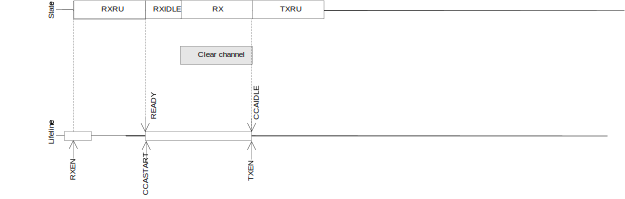
\includegraphics[width=\textwidth]{cca.png}
		\caption[Sende-Ablauf mit CCA Idle]{CCA Prüfung (Idle Event)\cite{nordic_semi_nrf_infocenter_radio_ieee_operation_2020}}
		\label{fig:CCAIDLEP2P}
	\end{minipage}
	\begin{minipage}[b]{0.5\textwidth}
		\centering
		\includegraphics[width=\textwidth]{cca_busy.png}
		\caption[Sende-Ablauf mit CCA Busy]{CCA Prüfung (Busy~Event)\cite{nordic_semi_nrf_infocenter_radio_ieee_operation_2020}}
		\label{fig:CCABUSYP2P}
	\end{minipage}
\end{adjustbox}
\end{figure}

\begin{figure} [H]
	\centering
	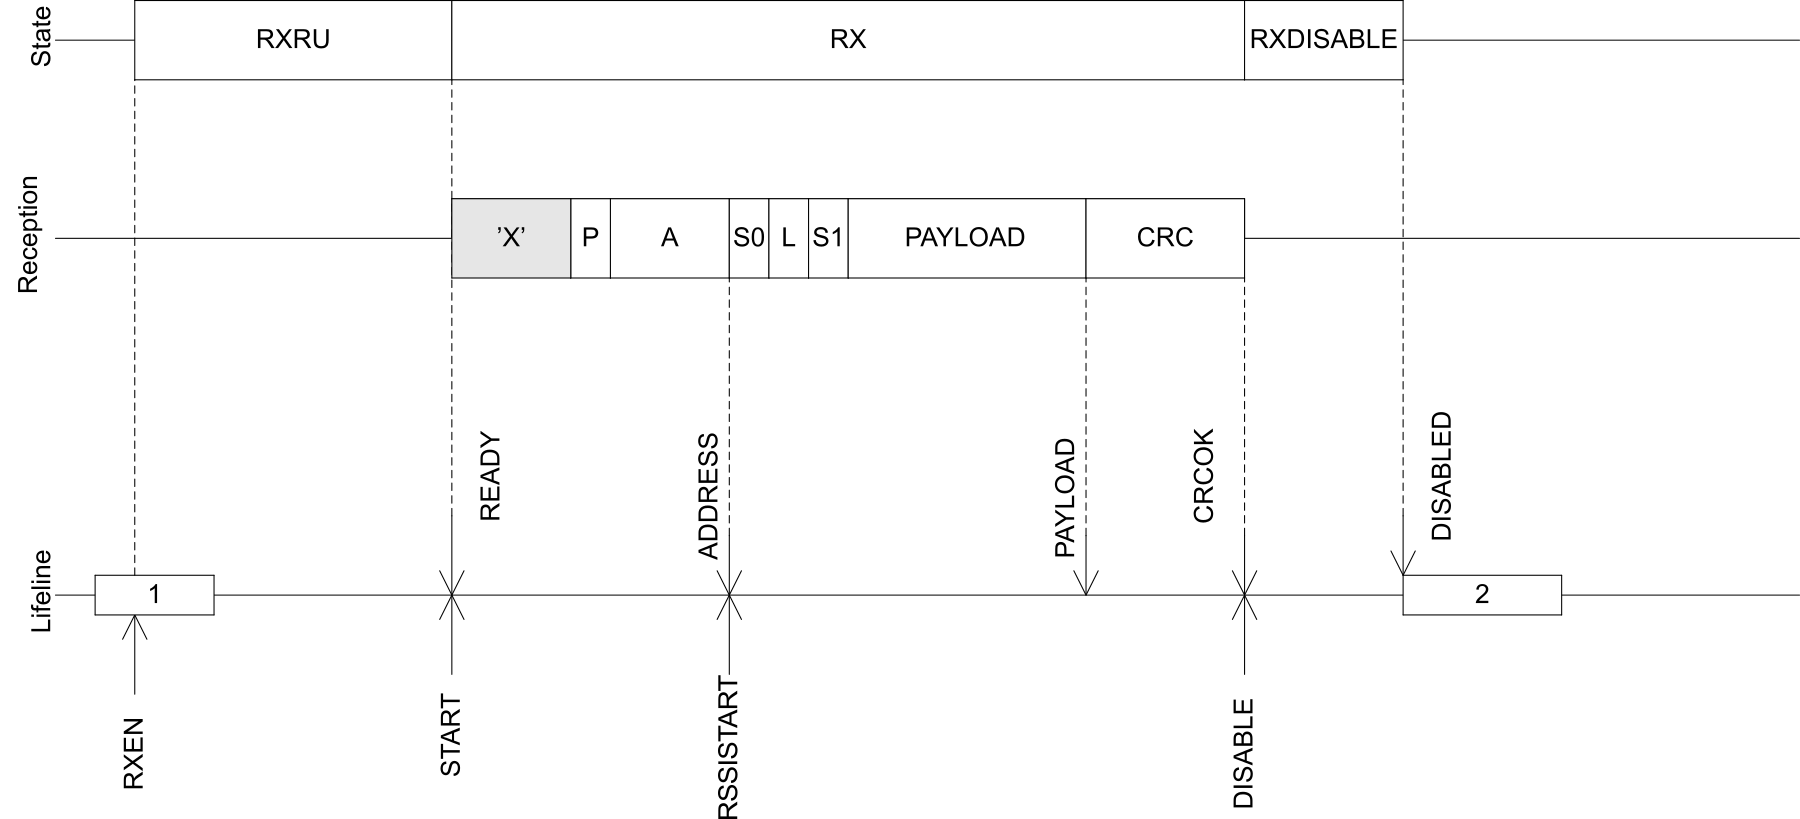
\includegraphics[width=1.0\textwidth]{nRF52840_Radio_Receive_Sequence_with_Shorts.png}
	\caption{Empfangs-Ablauf mit Verknüpfungen \cite{nordic_semi_nrf_infocenter_radio_receive_sequence_2020}}
	\label{fig:RadioReceiveSequP2P}
\end{figure}


Der Empfangsablauf eines Pakets wird in Abbildung \ref{fig:RadioReceiveSequP2P} dargestellt. Grundsätzlich ist der Ablauf gleich aufgebaut wie beim Senden eines Pakets. Nach dem Initiieren mittels RXEN-Befehl fährt der Empfänger hoch und wartet auf den Empfang eines Pakets. Nach Eingang einer Präambel-Sequenz wird das Adressfeld geprüft.
Dieses kann vorgängig so definiert werden, dass nur Pakete mit übereinstimmender Adresse empfangen werden.
Bei allen BLE-Modes erfolgt die Prüfung auf Hardware-Ebene (ohne Interaktion der CPU).
Beim \textit{IEEE802.15.4-Mode} steht dieses Feature jedoch nicht zur Verfügung. Das Vergleichen des Adressfeldes muss daher der Radio-Driver selbst übernehmen.

Um die Signalstärke (RSSI) des eingehenden Pakets zu messen, wird eine Verknüpfung zwischen dem \textit{Address-Event} und dem \textit{RSSIStart-Task} aktiviert.
Nach erfolgreicher Prüfung der CRC Checksumme wird mittels einer Verknüpfung des CRCOK-Event der Disable-Task ausgeführt.
Beim Empfang eines Pakets wartet der Radio-Driver während eines gewissen Timeouts auf den Disabled-Event.
Die Empfangsfunktion gibt die Restzeit des Timeouts in Millisekunden zurück, wodurch sich ein erfolgreicher Empfang prüfen lässt.
Das Bufferhandling übernimmt der Radio-Driver. Er erwartet beim Senden und Empfangen von Daten eine vordefinierte \textit{Radio-Packet-Structure}.
Es gilt zu beachten, dass die Daten erst nach dem End-Event  vollständig abgearbeitet wurden, da der Zugriff der Hardware via DMA (Direct Memory Access) erfolgt.
Ebenfalls wurde festgestellt, dass beim Wechsel zum oder vom  \textit{IEEE802.15.4-Mode} der Kanalwechsel vor dem Modewechsel erfolgen muss. Ansonsten werden keine Pakete empfangen. \cite{nordic_semi_nrf_infocenter_radio_receive_sequence_2020}


\subsection{Broadcasting Collisions Probability}\label{sec:BroadcastingCollissionsProbability}

Kollisionen entstehen, wenn mehrere Teilnehmer gleichzeitig auf dem selben Kanal (Frequenz) senden.
Dabei stören sich die beiden Sender und es besteht die Möglichkeit, dass der Empfänger keine Daten empfangen kann.
Wenn sich mehrere Teilnehmer neu mit dem Netz verbinden möchten, kann dies ebenfalls zu Problemen führen.
Leider können solche Störungen nicht immer vermieden werden.
In der vorliegenden Anwendung kann ein solcher Fall im Mockup-State entstehend.
Hier soll sich jeder Slave, welcher dem Master noch unbekannt ist, auf die Discovery-Anfrage des Masters melden.
Die Lösung ist, dass jeder Slave einen zufälligen Zeitpunkt zum Antworten auswählt.
Wie gross dieses Zeitfenster sein muss, in welchem ein Slave einen Zeitpunkt zufällig wählen darf, berechnet sich wie folgt:

Angenommen es gibt $N$ Teilnehmer, welche $t_a$ Sekunden brauchen, um eine Antwort zu senden.
Zusätzlich existieren $N_{ch}$ verschiedene Kanäle, auf welchen die Teilnehmer antworten können.
Die Wahrscheinlichkeit, dass sich zwei Sender im Zeitfenster $t_I$ Sekunden nicht überlappen $P_{miss}$, lässt sich gemäss Formel \ref{eq:BroadcastingMissProbability} bestimmen. \cite{rk_how_to_deal_with_broadcasting_collision_2020}

\begin{equation}\label{eq:BroadcastingMissProbability}
P_{miss} = (1- \frac{2 \cdot t_a}{N_{ch}} \cdot t_I)^{N-1}
\end{equation}

Die folgenden Werte wurden zur Berechnung des Zeitfensters im Mockup-State verwendet:

\begin{itemize}
	\item $N = 50$
	\item $t_a = 5ms$
	\item $N_{ch} = 3$
	\item $t_I = 1.2s$	
\end{itemize} 

Somit liegt die Wahrscheinlichkeit, dass alle 50 Nodes sich verfehlen bei 85\%. 

\subsection{Zeitsynchronisation}\label{sec:ZeitsynchronisationP2P}
Die Zeitsynchronisation wurde mittels einer Offset Kompensation gelöst.
Der Zeitgeber (Master) sendet seine Zeit (Timestamp) über einen Broadcast an alle Teilnehmer in der Umgebung.
Die Slaves vergleichen die empfangene Master-Zeit mit ihrer lokalen Zeit und errechnen den Unterschied (Offset) zwischen dem Master-Timestamp und Slave-Timestamp.
Somit können sie ihre Zeit an die des Masters angleichen. Das Prinzip ist relativ simpel, besitzt jedoch einige Ungenauigkeiten. Die Verzögerungszeit zwischen dem Auslesen des Master-Timestamps bis zum Empfangen und Vergleichen mit dem Slave-Timestamp ist kritisch.  

\begin{figure} [H]
	\centering
	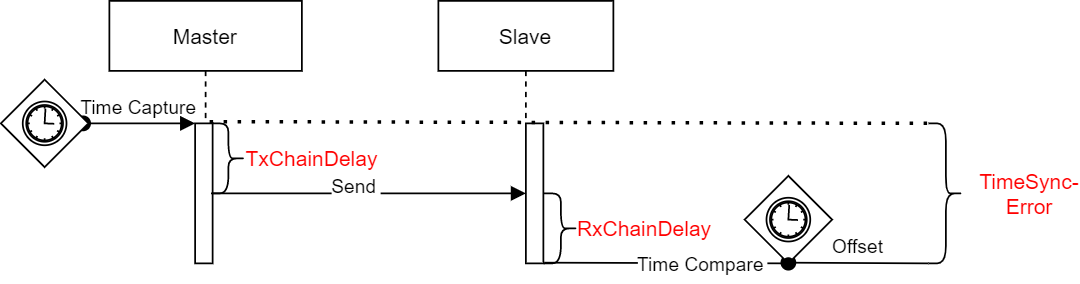
\includegraphics[width=1.0\textwidth]{Timesync_Basic.png}
	\caption{Zeitsynchronisation über Offset mit Fehler}
	\label{fig:TimesyncBasicwithErrorP2P}
\end{figure}

Wie in Abbildung \ref{fig:TimesyncBasicwithErrorP2P} ersichtlich ist, entsteht ab dem Auslesen der Zeit bis zum Senden eine Verzögerung die TxChainDelay sowie beim Empfänger die RxChainDelay. Das Ziel ist, diese Verzögerungen so gering wie möglich zu halten. 

\begin{figure} [H]
	\centering
	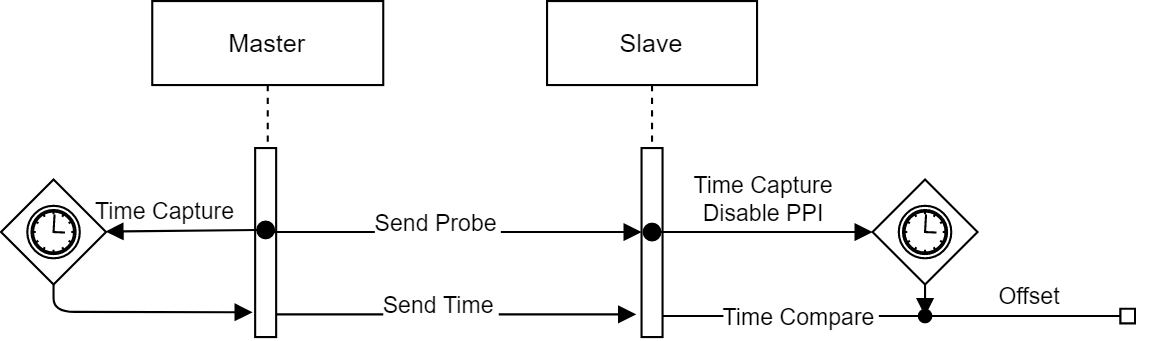
\includegraphics[width=1.0\textwidth]{Tiesync_Advanced.png}
	\caption{Zeitsynchronisation über Offset mit PPI}
	\label{fig:TimesyncwithPPIP2P}
\end{figure}

Die Lösung diese Problems wird in Abbildung \ref{fig:TimesyncwithPPIP2P} gezeigt. Der nRF52840 SoC verfügt über ein PPI (Programmable peripheral interconnect) Modul.
Mithilfe des PPI lassen sich verschiedene Events und Tasks direkt Verknüpfen, ohne dass die CPU dabei involviert ist.
Dies führt zu einer minimalen Verzögerung (ca. 1/16$\mu$s) zwischen Event und Task.
Dazu wird der Event, wenn ein Packet erfolgreich gesendet wurde (Radio-End-Event), mit dem Task zum Erfassen des Synctimers (Synctimer-Capture-Task) verknüpft.
Beim Slave wird der Event, wenn ein Packet erfolgreich Empfangen wurde (Radio-CRCOK-Event), mit dem Task zum Erfassen des Synctimers (Synctimer-Capture-Task) verknüpft.
Nach dem Empfang muss der Slave diesen PPI sofort deaktivieren, da ein direkt anschliessendes Paket ebenfalls ein Erfassen des Timers auslöst.
Der Master wird nach der Deaktivierung des PPI mit einem Folgepaket seine Master-Zeit dem Slave mitteilen, welche zum Zeitpunkt des Probe-Packets registriert wurde. Der Slave errechnet den Offset gemäss Formel \ref{eq:TimesyncOffsetSynctimeCalc} und die synchronisierte Zeit gemäss Formel \ref{eq:TimesyncSynctimeCalc}. \cite{nordic_semi_nrf_infocenter_ppi_2020}

\begin{equation}\label{eq:TimesyncOffsetSynctimeCalc}
T_{Offset} =  T_{Master} - T_{Slave} 
\end{equation}

\begin{equation}\label{eq:TimesyncSynctimeCalc}
T_{Sync} =  T_{Slave} + T_{Offset} 
\end{equation}

Zur Verifizierung der Zeitsynchronisation wurde ein Oszilloskop an jeweils einen GPIO-Pin des Masters und an einen Pin des Slaves angeschlossen. Auf dem Master und Slave wurden nacheinander Timer-Interrupts registriert, welche relativ zur synchronisierten Zeit auf dem Master und Slave genau gleichzeitig auslösen. Mithilfe eines PPI-Kanals wurde der Interrupt-Event auf den GPIO-Pin verknüpft.
Beim Auslösen des Interrupts wird der Zustand des GPIO-Pins invertiert.
Dadurch wird die Abweichung präzise auf dem Oszilloskop ersichtlich.

\begin{figure} [H]
	\centering
	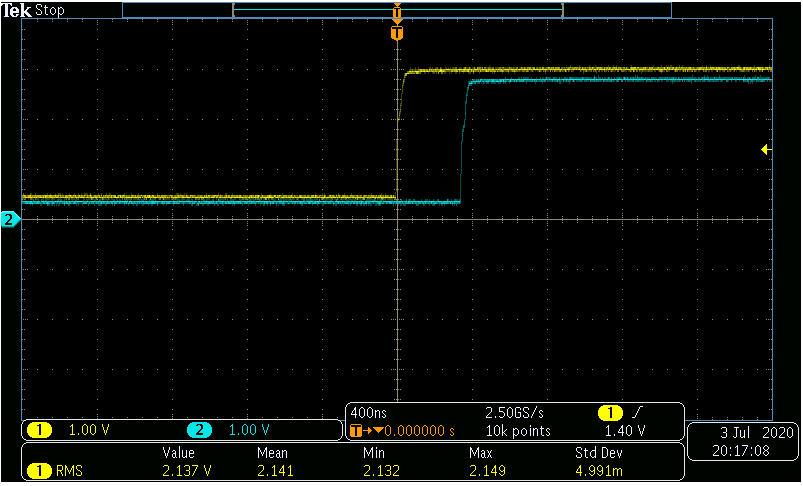
\includegraphics[width=1.0\textwidth]{Messungen Timesync (100ns 1200ns).png}
	\caption{Verifizierung Zeitsynchronisation mittels Oszilloskop.}
	\label{fig:TimesyncVerifikationP2P}
\end{figure}

Abbildung \ref{fig:TimesyncVerifikationP2P} zeigt den Signalverlauf der GPIOs von Master (gelb) und Slave (blau).
Anfänglich lagen die Abweichungen im Bereich von ca. 40$\mu$s.
Durch die Wiederholungen der Messung konnte dieser Fehler als systematisch identifiziert werden.
Mithilfe einer Korrektur um 40$\mu$s konnte die Genauigkeit in den Bereich von 100ns bis 1200ns beschränkt werden. Eine Abweichung der Zeitsynchronisation von ca. 1$\mu$s sollte genügend genau sein, damit die Messungen als gute Grundlage für die Statemachine aus Abschnitt \ref{sec:SoftundFirmware} dienen können. 
 
\subsection{Webserver}\label{subsec:DjangoWebserver}
Damit die P2P-Testinfrastruktur visualisiert und mit einem schönen User Interface gesteuert werden kann, wurde ein Webserver aufgesetzt.
Das Ziel ist, auf einem Rechner unter einer Web-Adresse einen Webserver zu erreichen, welche es ermöglicht alle Einstellungen über eine Serielle Schnittstelle dem BMN mitzuteilen.
Damit wird es möglich den Ablauf bequem über den Webserver zu steuern.

\subsubsection{Django}\label{subsubsec:Django}
Als Grundlage für den Webserver dient eine Django Instanz.
Django ist ein open-source Webframework, welches auf dem Model-View-Controller Prinzip basiert und in der Programmiersprache Python geschrieben wurde.
Das Framework hat sein eigenes Benennungssystem für alle Funktionen und Komponenten.
Zum Beispiel werden HTTP-Antworten als Views bezeichnet.
Ein grosser Vorteil von Django ist die Administrationsseite.
Diese ist Bestandteil des Projekts und dient dazu die Models zu verwalten.
Models sind Objekte, die in einer Datenbank des Webservers gespeichert werden. Die gängigsten Datenbanksysteme, wie z.B. SQLLite sind in Django integriert und können aktiviert bzw. implementiert werden \cite{django_django_2020}.
In der Tabelle \ref{table:FeaturesDjango} sind die wichtigsten Features von Django aufgelistet.


\begin{table}[h]
\centering
\begin{tabular}{|l|l|l|} 
\hline
Einfacher Syntax (Python) & Model-View-Controller & Administrations Seite \\ 
\hline
Model-View-Controller & Eigener Webserver & Gängigste Datenbanken \\ 
\hline
HTTP Bibliothek & Python Unit Test Framework & Models für Datenbank \\
\hline
\end{tabular}
\caption{Features Django Webserver \cite{django_django_2020}}
\label{table:FeaturesDjango}
\end{table}

\subsubsection{Software Grundlagen}\label{subsubsec:SoftwareGrundlagen}
Bei einer gewöhnlichen datengesteuerten Webseite wartet die Webanwendung auf eine HTTP-Anfrage des Browsers.
Wird ein Anfrage empfangen, so bestimmt die Anwendung, auf Grundlage der URL, ob ein GET oder POST Event ausgelöst wird.
Je nach Anfrage wird somit aus einer Datenbank gelesen oder es wird in die Datenbank geschrieben.
Die Anwendung sendet danach eine Antwort an den Webbrowser, wobei häufig eine HTML-Seite erzeugt wird, um die Antwort darzustellen. Diese Schritte sind in Django, wie in der Abbildung \ref{fig:DjangoAblauf} aufgeführt, in separaten Dateien zusammengefasst. Dies werden unterhalb kurz beschrieben.

\begin{figure} [H]
	\centering
	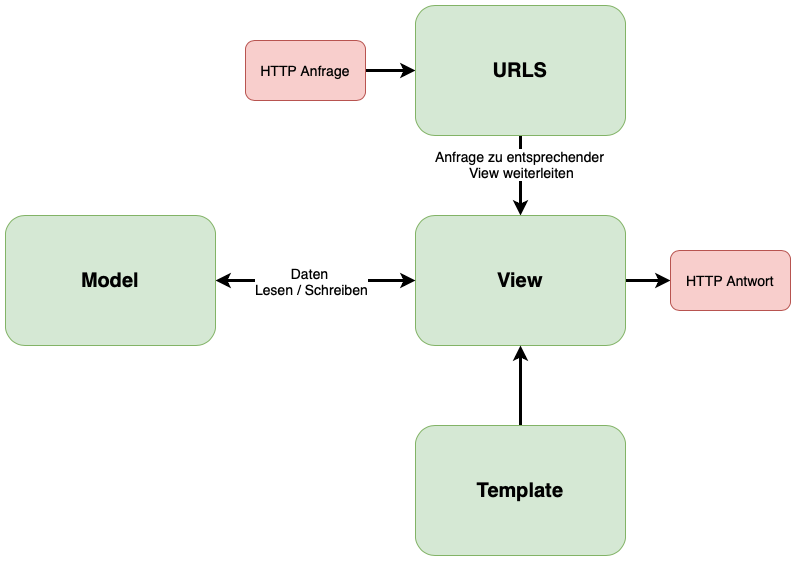
\includegraphics[width=0.76\textwidth]{Django Ablauf.png}
	\caption{Django Funktionen \cite{mdn_web_docs_django_2019}}
	\label{fig:DjangoAblauf}
\end{figure}

\paragraph{URLs}
Die URL Datei leitet die Anfrage an die entsprechende View weiter. Damit dies gelingt wird ein URL-Mapper eingesetzt.
Dieser dient dazu, die Anfrage so zu interpretieren, damit die richtige View aufgerufen wird.
Zusätzlich erkennt der URL-Mapper Zeichenketten und Ziffern in der URL und kann diese abgleichen und anschliessend als Daten an die View-Funktion weitergeben.

\paragraph{Views}
Die View ist eine Request-Handler-Funktion, die HTTP-Anfragen empfängt und zurückgibt.
Die View kann über die Model Funktion auf Daten in der Datenbank zugreifen.
Über die Template-Funktion beschreibt die View schlussendlich, wie die HTTP-Antwort formatiert werden muss.

\paragraph{Models}
Ein Model ist ein Python Objekt, welches die Struktur der Daten einer Anwendung definiert. Darüber hinaus stellt die Funktion die Mittel wie beispielsweise das Hinzufügen, Löschen oder Ändern bereit, um die Daten in der Datenbank zu verwalten.
Die Model Funktion ist somit die Schnittstelle zur Datenbank.

\paragraph{Templates}
Das Template ist eine Textdatei, in der die Struktur oder das Layout einer zugehörigen HTML-Seite definiert wird.
Für die Struktur werden Platzhalter zur Darstellung des eigentlichen Inhalts verwendet.
Demnach kann die View-Funktion mit Hilfe vom Templates eine dynamische HTML-Seite erzeugen und diese mit Daten der Model-Funktion füllen.

\subsubsection{Aufbau Software}\label{subsubsec:SoftwareAufbau}
Der Aufbau des Django Weberservers für die P2P-Testinfrastruktur ist in Abbildung \ref{fig:FunktionenP2PWebserver} ersichtlich.

\begin{figure} [H]
	\centering
	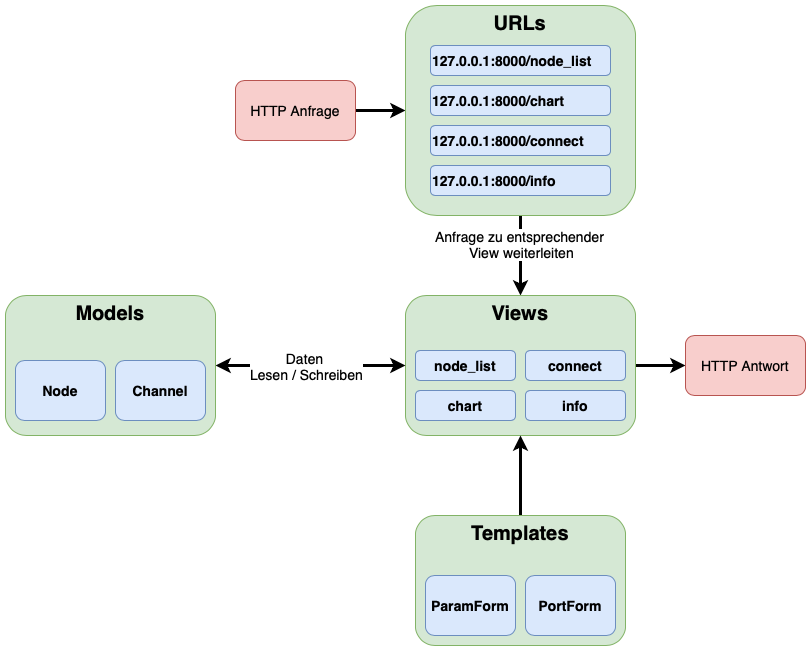
\includegraphics[width=0.8\textwidth]{DjangoSoftwaredoku.png}
	\caption{Funktionen P2P Webserver}
	\label{fig:FunktionenP2PWebserver}
\end{figure}


\paragraph{URLs}
In der folgenden Tabelle sind alle URLs aufgelistet, welche verwendet wurden, um auf die entsprechenden Views zu verweisen.

\begin{itemize}
	\item 127.0.0.1:8000/node\textunderscore list \hspace{2.5mm} referenziert auf die View node\textunderscore list
	\item 127.0.0.1:8000/chart \hspace{10mm} referenziert auf die View chart
	\item 127.0.0.1:8000/connect \hspace{6mm} referenziert auf die View connect
	\item 127.0.0.1:8000/info \hspace{12.5mm} referenziert auf die View info
\end{itemize} 

\paragraph{Views}
Es wurden vier Views im P2P-Webserver erstellt, die die Schnittstellen zu den Forms, den Models und den HTML-Dateien bilden:
\begin{itemize}
	\item node\textunderscore list
	\item chart
	\item connect
	\item info
\end{itemize} 
Die Bedienung der einzelnen Seiten wurde im Kapitel \ref{sec:InbetriebnahmeBedienungP2P} bereits erläutert.

\paragraph{Models}
Für die Speicherung der Daten vom P2P Master sind die folgenden zwei Objekte verfügbar: 
\begin{itemize}
	\item Node
	\item Channel
\end{itemize} 

Diese zwei Objekte sind miteinander verknüpft.
Wenn ein Objekt Node erstellt wird, können die dazugehörigen Channel Informationen ebenso erstellt werden.
Dadurch ist eine klare Struktur gegeben.
Über das Objekt Node können die verschiedenen Channel Informationen abgerufen werden.

Folgende Parameter können dem Objekt Node als Information mitgegeben werden:
\begin{itemize}
	\item MAC Adresse
\end{itemize} 

Folgende Parameter können dem Objekt Channel als Information mitgegeben werden:
\begin{itemize}
	\item Channel Nummer
	\item Signal to noise ratio
	\item Packetloss
	\item Node ID
\end{itemize}

\paragraph{Templates}
Als Template wurden zwei verschiedene Django Forms erstellt. Die eine Form ist eine Anordnung an Eingabefeldern, die frei bestimmt werden können. Die Dropdown Auswahlmöglichkeiten sind in der Tabelle \ref{table:TabelleAuswahlfelder} aufgelistet.

\begin{table}[h]
\centering
\begin{tabular}{|l|l|l|l|} 
\hline
\multicolumn{4}{|c|}{\textbf{Auswahlfelder} } \\ 
\hline
\multicolumn{1}{|c|}{\textbf{Mode} } & \multicolumn{1}{c|}{\textbf{CSMA CA} } & \multicolumn{1}{c|}{\textbf{Tx Power} } & \multicolumn{1}{c|}{\textbf{Port} } \\ 
\hline
1 Mbit/s Nordic radio mode & Off & 0 dB & Disconnect \\ 
\hline
2 Mbit/s Nordic radio mode & Ed Mode & 1 dB & COM 1 \\ 
\hline
1 Mbit/s BLE & Carrier Mode & 2 dB & COM 2 \\ 
\hline
2 Mbit/s BLE & Carrier and Ed Mode & 3 dB & COM 3 \\ 
\hline
Long range 125 kbit/s TX & Carrier or Ed Mode & 4 dB & COM 4 \\ 
\hline
Long range 500 kbit/s TX &  & 5 dB & COM 5 \\ 
\cline{1-1}\cline{3-4}
IEEE 802.15.4-2006 250 kbit/s &  & 6 dB & COM 6 \\ 
\cline{1-1}\cline{3-4}
\multicolumn{1}{l}{} &  & 7 dB & COM 7 \\ 
\cline{3-4}
\multicolumn{1}{l}{} &  & 8 dB & \textbf{...}  \\
\cline{3-4}
\end{tabular}
\caption{Tabelle Auswahlfelder}
\label{table:TabelleAuswahlfelder}
\end{table}


Für die Eingabe der Parameter, die auf dem P2P Master eingestellt werden können, ist die Form \textit{ParamForm} mit folgenden Eingabefeldern verfügbar:
\begin{itemize}
	\item Start Channel \hspace{5mm} -> Integer Feld
	\item Stop Channel \hspace{6mm} -> Integer Feld
	\item Size \hspace{22.3mm} -> Integer Feld
	\item Mode \hspace{19.5mm} -> Drop Down Auswahlfeld
	\item CSMA CA \hspace{10.5mm} -> Drop Down Auswahlfeld
	\item Tx Power \hspace{13mm} -> Drop Down Auswahlfeld
\end{itemize}

Für die Auswahl des Ports der Seriellen Verbindung zum Master ist die Form \textit{ParamForm} mit folgenden Eingabefeldern verfügbar:
\begin{itemize}
	\item  Port \hspace{22mm} -> Drop Down Auswahlfeld
\end{itemize}

In Abbildung \ref{fig:ParamForm} und \ref{fig:PortForm} sind die Eingabe Forms ersichtlich. Die Daten werden mit einem Button, der ein HTTP-POST Ereignis auslöst, an die entsprechende View weitergeleitet.

\begin{figure} [H]
	\centering
	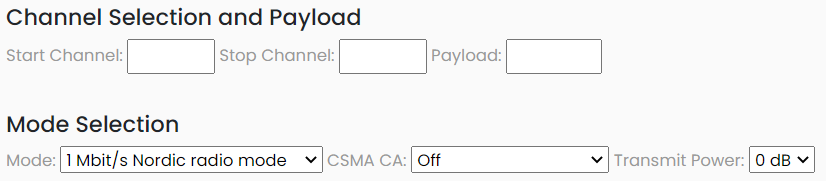
\includegraphics[width=0.8\textwidth]{ParamForm.png}
	\caption{Parameter Form}
	\label{fig:ParamForm}
\end{figure}

\begin{figure} [H]
	\centering
	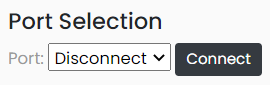
\includegraphics[width=0.3\textwidth]{PortForm.png}
	\caption{Port Form}
	\label{fig:PortForm}
\end{figure}

\paragraph{Serielle Kommunikation:}
Die serielle Kommunikation wird mithilfe der Python Bibliothek \textit{PySerial} aufgebaut. Auf der P2P-Webserver Seite Connect kann der Port ausgewählt werden, an dem der P2P-Master angeschlossen ist. Sobald die Verbindung zum Master besteht, wird ein separater Python Thread gestartet. In diesem Thread wird in einem while-loop das Serielle Interface permanent ausgelesen. Sobald der Master einen neuen Mess-Report schickt, wird dieser ausgewertet und die Objekte Node und Channel werden anhand des Reports erstellt. In Abbildung \ref{fig:AblaufDjangoSerial} ist dieser Ablauf ersichtlich.

Die erhaltenen Daten werden in der View Node\textunderscore List in einer dynamischen Tabelle, die jede Sekunde aktualisiert wird, angezeigt. Zudem ist in der View Chart eine Visualisierung der Daten ersichtlich. Die Messergebnisse werden mit Hilfe der Bibliothek \textit{PlotLy} dargestellt. 

\begin{figure} [H]
	\centering
	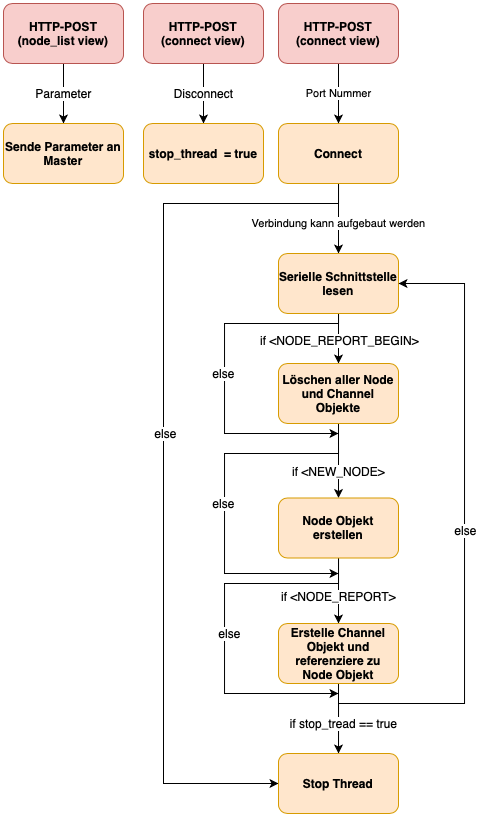
\includegraphics[width=0.63\textwidth]{Ablauf Django Serial.png}
	\caption{Ablauf Django Serial}
	\label{fig:AblaufDjangoSerial}
\end{figure}

\newpage
\section{Schluss}\label{sec:SchlussP2P}

Abschliessend wird eine kurze Validierung und Verifizierung der Messresultate, sowie eine Schlussbetrachtung vorgenommen.

\subsection{Validierung}\label{subsec:P2PValidierung}
Die vorgegebenen Ziele zur Erfassung des SNR und Paketverlusts konnten erreicht werden.
Das Tool erfüllt mittels der grafischen Oberfläche seinen Zweck als universell einsetzbares Messwerkzeug.
Das Erfassen des SNRs funktioniert jedoch nicht immer optimal.
Durch Störeinflüsse, welche sich schnell ändern (WLAN etc.) kann es vorkommen, dass die Angabe des SNRs nicht korrekt erfolgt.
Die Ergebnisse des Paketverlusts sehen allerdings valide aus. 

\todo[inline]{Cyrill: Validierung ausführlicher oder ganz weglassen.}

\subsection{Verifizierung}\label{subsec:P2PVerifizierung}
Die Messwerte korrelieren mit denjenigen des Radio-Test-Examples, welches einen ähnlichen Zweck erfüllt \cite{nrf_connect_sdk_radio_test_example_2020}.
Die Messresultate sind jedoch stark von äusseren Störeinflüssen abhängig. Somit wird eine exakte Verifizierung fast unmöglich.

\todo[inline]{Cyrill: Verifizierung ausführlicher oder ganz weglassen.}


\subsection{Fazit}\label{subsec:FazitP2P}
\paragraph{Firmware}
Die Analyse des MAC-Layers und die Umsetzung der Testinfrastruktur hat viele Erkenntnisse im Bereich der hardwarenahen Programmierung gebracht. Durch die Erarbeitung der Firmware sind viele Module (Zeitsynchronisation, Statemachine, CLI, etc.) geschaffen worden, welche in weitere Programme integrierbar sind. Somit ergab sich eine optimale Grundlage, um in die Netzwerk-Stacks, welche auf dem MAC-Layer basieren, einzutauchen.

\paragraph{Webserver}
Die Entwicklung eines Webservers für die Bedienung der P2P-Testinfrastruktur war eine sehr lehrreiche Erfahrung. Bis anhin waren nur die Programmiersprachen C und C\texttt{++} bekannt. Das Erlernen und Anwenden von Python, HTML und Javascript für den Aufbau und die Darstellung des Webservers waren sehr intensiv aber auch lehrreich. Gewisse Funktionen vom Webserver könnten verbessert werden. Dazu gehören folgende:

\begin{itemize}
	\item Das Aktualisieren der Tabellen und der Charts wird im Sekundentakt gemacht. Es wäre besser die Aktualisierung auszuführen sobald der Master Node meldet, dass er mit dem Report fertig ist.
	\item Das Aktualisieren der Charts geschieht, indem die ganze Seite neu geladen wird. Die einzelnen Charts neu zu zeichnen, ohne die Seite neu zu laden, wäre effektiver.
	\item Die Auswahl des COM-Ports ist fix hinterlegt. Eine dynamische Auswahl, die zeigt welche Geräte angeschlossen sind, wäre in der Bedienung komfortabler.
\end{itemize}



\pagebreak

\vspace*{4cm}
\begin{center}
\part{Mesh Benchmark Konzept und Testumgebung}\label{MeshBenchmarkKonzeptundTestumgebung}
\end{center}
\vspace*{\fill}
\clearpage

\section{Benchmark Konzept Mesh Netzwerke}\label{sec:BenchmarkKonzeptMeshNetzwerke}
Um die Performance der drei Mesh Stacks zu vergleichen wurde ein einheitliches Benchmark Konzept erarbeitet. Dieses definiert die Mesh Parameter, Testumgebungen, den Ablauf sowie sämtliche Messgrössen und Messreihen. Nachfolgend wird detailliert auf dieses Konzept eingegangen.

\subsection{Konzeptschema}\label{subsec:KonzeptschemaMesh}

Für den Vergleich der 3 Mesh Netzwerkstacks Bluetooth Mesh (BT Mesh), Thread und Zigbee wird ein vom Mesh Protokoll unabhängiges Testkonzept umgesetzt welches in der Abbildung \ref{fig:MeshTestKonzept} als Konzeptschema dargestellt ist.
Die Benchmark Slave Nodes (BSN) in der Abbildung als Sensoren und Aktoren mit unterschiedlichen Funktionalitäten dargestellt, bilden zusammen mit dem Benchmark Master Node (BMN) das zu testende Mesh Netzwerk.
Innerhalb des Netzwerks wird dessen Organisation vom jeweiligen Protokoll sichergestellt.
Das Testnetzwerk soll ein realitätsnahes Netzwerk nachbilden.
Beispielsweise wird eine Hausautomation in einem Einfamilienhaus als Referenz angenommen in welchem jeweils nur gewisse Nodes untereinander Applikationsdaten austauschen.
Ein Lichtschalter kommuniziert nur mit einer Lichtquelle und umgekehrt.
Der selbe Lichtschalter tauscht jedoch keine Applikationsdaten mit dem Temperatursensor aus.
Trotzdem bilden die Nodes zusammen ein Mesh Netzwerk.
Diese unterschiedlichen Beziehungen innerhalb des Mesh Netzwerks sind in der Abbildung \ref{fig:MeshTestKonzept} bereits angedeutet und werden im Abschnitt \ref{subsubsec:MeshBeziehungen} noch genauer beschrieben.

\begin{figure}[h]
	\centering
	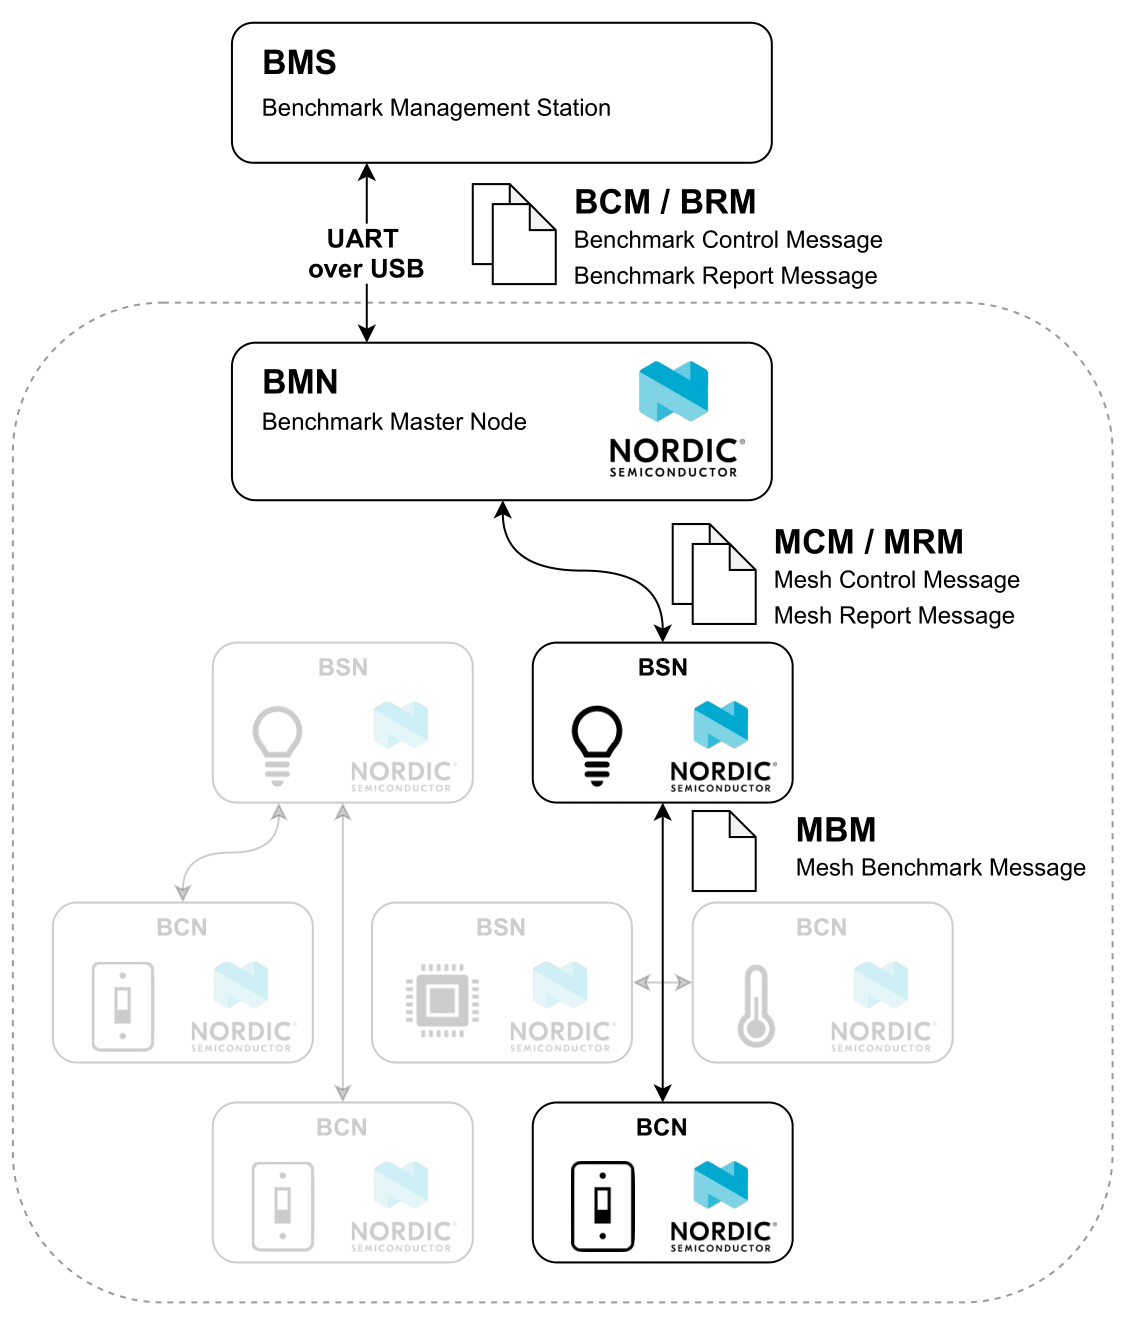
\includegraphics[width=0.6\textwidth]{Mesh_Testkonzeptschema.png}
	\caption{Konzeptschema für den Ablauf eines Mesh Benchmarks.}\label{fig:MeshTestKonzept}
\end{figure}

Die Benchmark Management Station (BMS) welche mit dem BMN via USB/UART kommuniziert, ist zuständig für die Verwaltung und Verarbeitung der Benchmarks. Während eines Benchmark Prozesses sollen sämtliche Messungen jedoch unabhängig von der BMS durchgeführt werden damit allfällige Latenzzeiten der USB/UART Verbindung die Resultate nicht verfälschen.

\subsubsection{Messages}\label{subsubsec:Messages}
In der Abbildung \ref{fig:MeshTestKonzept} sind verschiedene Messages dargestellt. Dabei handelt es sich um die Nachrichten die zwischen den einzelnen Teilen des Testaufbaus versendet werden und schliesslich einen Benchmark ausmachen. Die Messages besitzen Funktionen:

\paragraph{Mesh Benchmark Message (MBM)}
Die MBM ist jene Message welche die eigentlichen Messdaten produziert und diese sogleich unter den BSN (Mesh Knoten) überträgt. Anhand dieser Messages werden die Parameter für den Vergleich der Protokolle gemäss Abschnitt \ref{subsec:VergleichswerteundMessgrössenMesh} erfasst. Bei den MBM handelt es sich also um eine Sammlung von Messages welche je nach gewünschtem Messwert in Form und Anzahl unterschiedlich ausfallen können.

\paragraph{Mesh Control Message (MCM)}
Die MCM beinhaltet die Parameter für die Benchmarks welche vom BMN an alle BSN übertragen werden. Ausserdem werden damit Kontrollbefehle für die Benchmarks wie beispielsweise \textit{Start/Stop} sowie \textit{Laufzeit, Wiederholrate usw.} übertragen.

\paragraph{Mesh Report Message (MRM)}
Die MRM ist jene Message welche die Messwerte von den BSN an den BMN übertragen. Gleichzeitig wird damit auch gleich signalisiert, dass die Messung abgeschlossen wurde und mögliche Fehler oder sonstige Status übermittelt.

\paragraph{Benchmark Control Message (BCM)}
Die BCM beschreibt die Nachrichten welche zur Steuerung eines Benchmarks von der BMS her dienen. Dabei handelt es sich um Befehle wie beispielsweise \textit{Start/Stop}. Die BCM werden via serieller USB-UART Schnittstelle von der BMS zum BMN übertragen.

\paragraph{Benchmark Report Message (BRM)}
Die BRM beschreiben Nachrichten welche den Status oder die Ergebnisse eines Benchmarks aus dem Mesh zurück an die BMS melden. Sie werden vom BMN initiiert und gelangen über eine die selbe USB-UART Schnittstelle wie die BCM zum BMS. Die BRM wird erst nach Abschluss des Benchmarks initiiert. Zuvor werden die Messdaten auf dem BMN zwischen gespeichert.


\subsubsection{Nodes}\label{subsubsec:Nodes}
Wie bereits angedeutet und in Abbildung \ref{fig:MeshTestKonzept} gezeigt, kann im Mesh Benchmark zwischen den folgenden 3 Node Typen unterschieden werden.

\paragraph{Benchmark Master Node (BMN)}
Der Benchmark Master Node bildet den zentralen Zugriffspunkt zum Mesh Netzwerk für den Benchmark. Über ihn werden Control und Report Messages versendet und empfangen. Je nach Mesh Protokoll fungiert er zugleich als Mesh Leader (Thread) respektive Coordinator (Zigbee).

\paragraph{Benchmark Client Node (BCN)}
Der Benchmark Client Node repräsentiert beispielsweise einen Schalter in einer Lichtsteuerung. Im Benchmark Kontext ist er jene Instanz die MBM versendet.

\paragraph{Benchmark Server Node (BSN)}
Das Pendant zum BCN stellt der BSN dar. Er steht beispielsweise für eine Lichtquelle. Im Benchmark Kontext empfängt er die MBM die vom BCN versendet werden.


\subsection{Testszenarien}\label{subsec:TestszenarienMesh}

Die Benchmarks der Mesh Protokolle sollen mit unterschiedlichen Bedingungen getestet werden wobei grundsätzlich eine reelle Anwendung nachgebaut werden soll. Zum einen gibt es unterschiedliche Beziehungen innerhalb des Mesh Netzwerks, zum anderen werden Testumgebungen unterschieden.

\subsubsection{Mesh Beziehungen}\label{subsubsec:MeshBeziehungen}

Innerhalb eines Mesh Netzwerks können 4 Beziehungen zwischen den Nodes für die Benchmarks unterschieden werden. Üblicherweise kommen mehrere oder sogar alle 4 Beziehungen innerhalb eines Netzwerkes gleichzeitig zum Einsatz. Abbildung \ref{fig:MeshTestBeziehungen} zeigt die Beziehungen.

\begin{itemize}
 	\item \textcolor{red}{Rot} stellt eine einfache P2P Verbindung ohne Hop dar. Beispielweise schaltet ein einzelner Schalter eine einzelne, definierte Lichtquelle
 	\item \textcolor{orange}{Orange} ist eine many-to-one Verbindung in welcher mehrere Lichtschalter die selbe Lichtquelle schalten.
 	\item \textcolor{cyan}{Blau} ist eine klassiche one-to-many Topologie dargestellt in welcher beispielsweise ein Schalter mehrere Lichtquellen bedient.
 	 \item \textcolor{green}{Grün} dargestellt ist eine indirekte P2P Verbindung mit. Das bedeutet, dass Schalter und Lichtquelle keine direkte Verbindung zueinander haben und daher Mesh-typisch via einem oder mehreren Hops kommuniziert.
\end{itemize}


\begin{figure}[H]
	\centering
	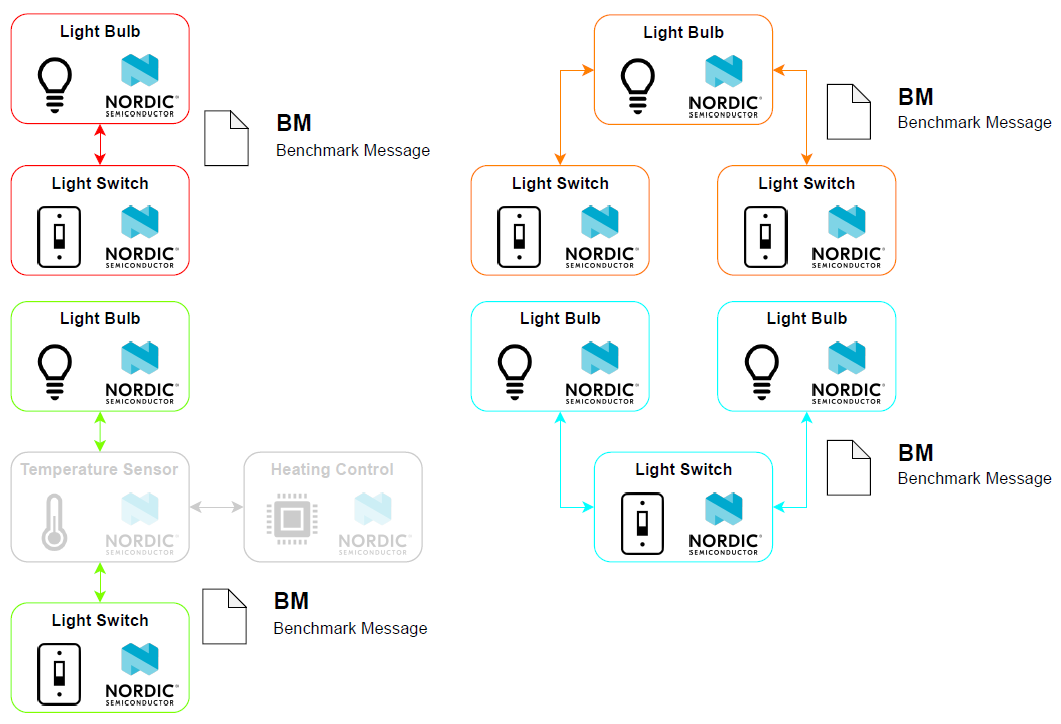
\includegraphics[width=1.0\textwidth]{Mesh_Test_Beziehungen.png}
	\caption{Beziehungen zwischen den Mesh Nodes innerhalb eines Benchmarks.}\label{fig:MeshTestBeziehungen}
\end{figure}


\subsubsection{Testumgebungen und Messaufbau}\label{subsubsec:TestumgebungenundMessaufbau}

Unterschiedliche Testumgebungen sollen die Benchmarks und schlussendlich den Vergleich der 3 Mesh Protokolle aussagekräftiger machen.
Nachfolgende Umgebungen mit den entsprechenden Eigenschaften sollen getestet werden.
Die Abbildungen zu den Testumgebungen zeigen jeweils die Platzierung der Nodes sowie deren Funktion und Gruppen Zugehörigkeit. Die Farbe Grün identifiziert den Node als Client Node während Blau für einen Server Nodes steht. Die Nummerierung zeigt welcher Node zu welcher Adressgruppe gehört. Ein Client Node in Gruppe 1 sendet jeweils Nachrichten zu allen Server Nodes in der selben Gruppe.

\paragraph{Labor}
Der Laboraufbau ist ein Extremtest welcher die Leistungsgrenzen der Protokollstacks ausloten soll. Dabei werden die Nodes auf einem Raster gemäss Abbildung \ref{fig:AnordnungLaborTestumgebungMessumgebung1} angeordnet. Die genauen Abmessungen sind der Abbildung zu entnehmen.
\begin{itemize}
	\item Testaufbau unter Laborbedingungen auf engstem Raum.
	\item Ausgeglichene Anzahl Sensoren und Aktoren.
	\item Sehr Hohe Node-Dichte.
	\item Geringe bis keine Störbeeinflussung durch die Umgebung zu  erwarten.
	\item Die Mesh-Beziehungen werden künstlich bestimmt sodass einfache P2P Verbindungen mit oder ohne Hop entstehen.
\end{itemize}


\begin{figure}[H]
\centering
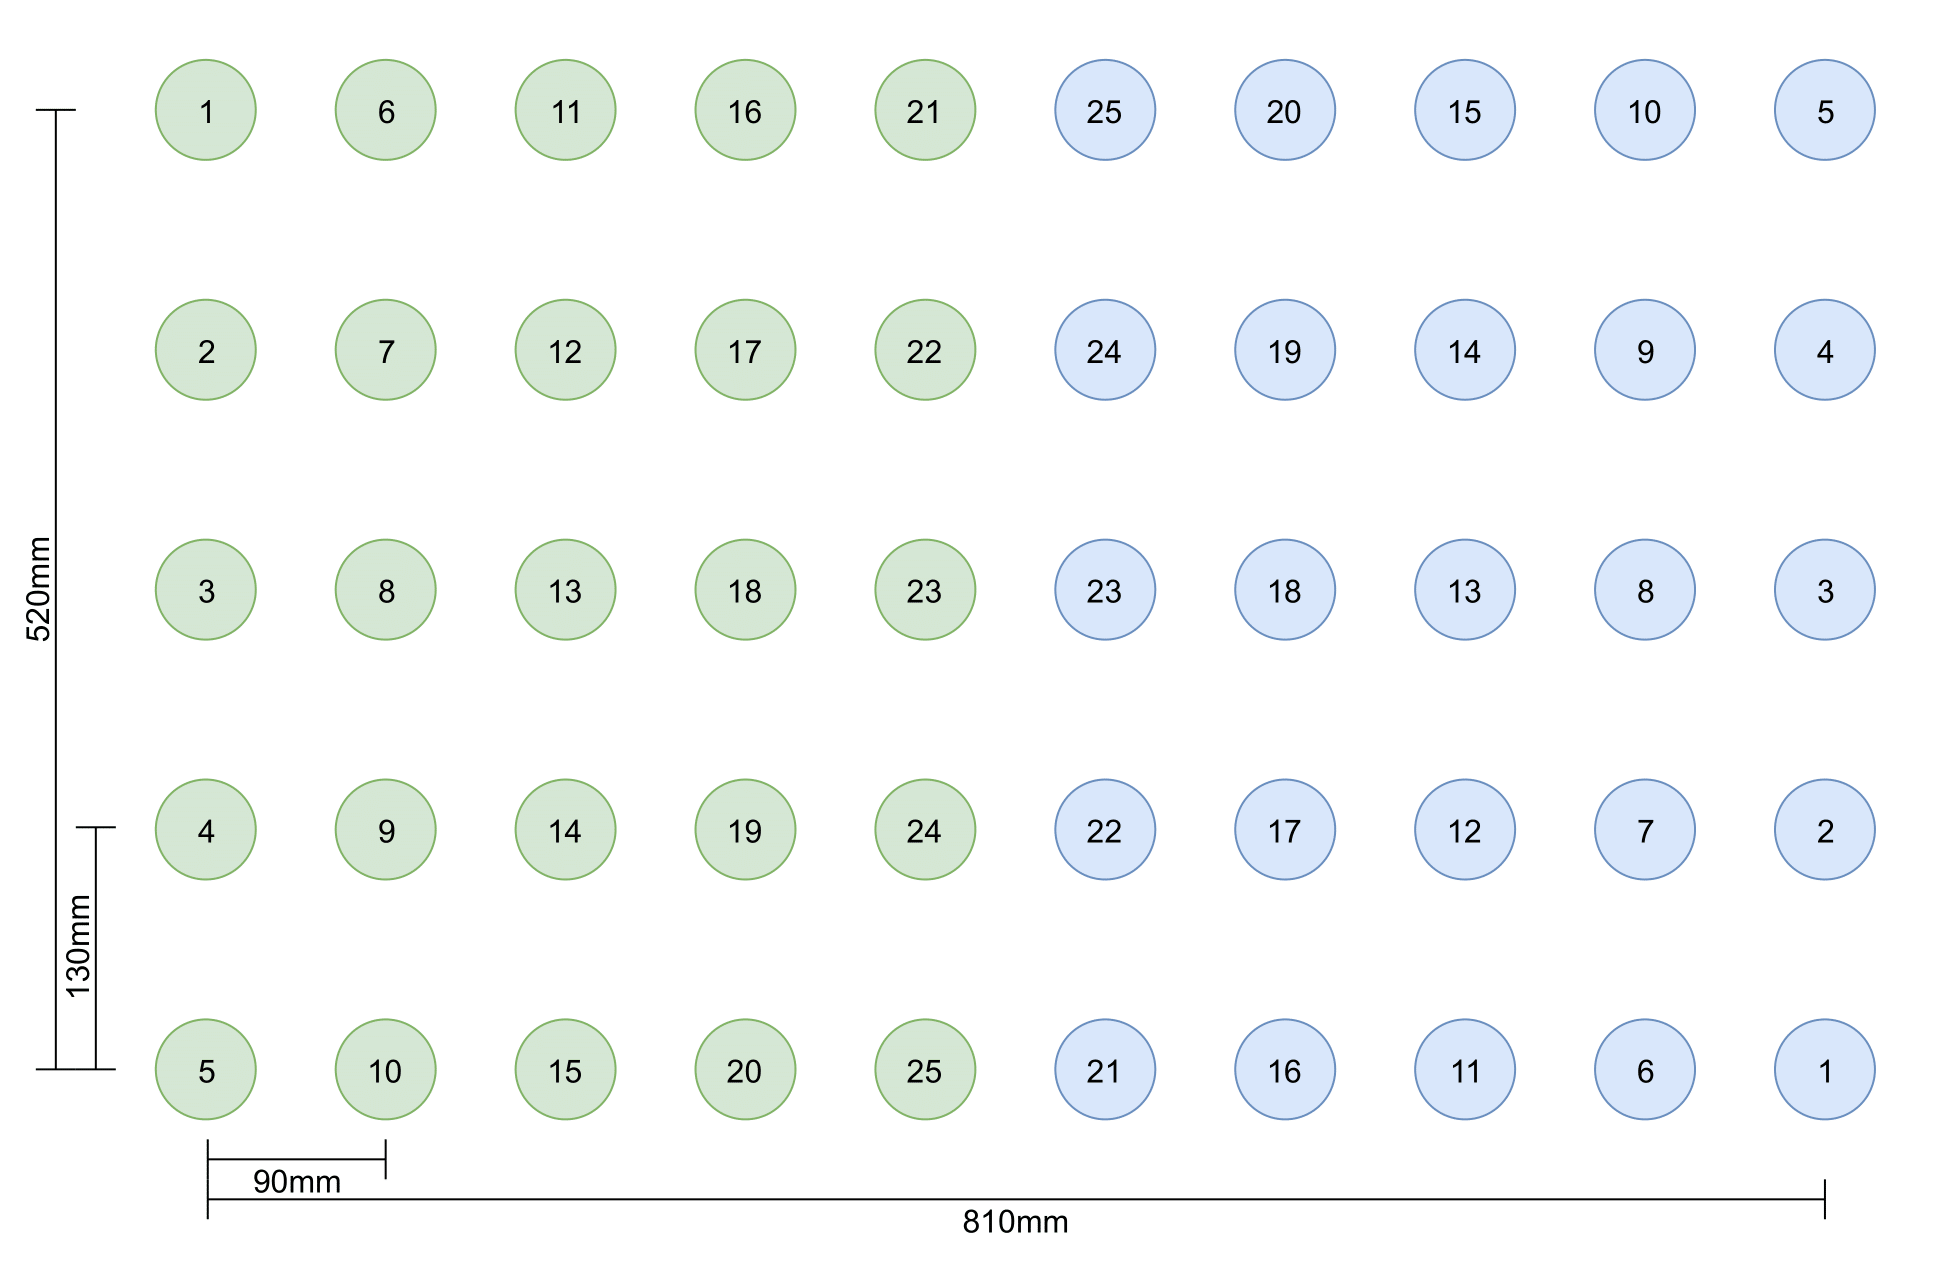
\includegraphics[width=0.7\textwidth]{Testaufbau_Labor.png}
\caption{Anordnung Labor Testumgebung, Messumgebung 1}\label{fig:AnordnungLaborTestumgebungMessumgebung1}
\end{figure}

\paragraph{Einfamilienhaus}
Die Testgeräte werden in einem Einfamilienhaus installiert und repräsentieren damit eine flächendeckende Heim-Automatisierung. Folgende Eingenschaften soll diese Messung abdecken:
\begin{itemize}
	\item Einfamilienhaus über mehrere Etagen.
	\item Node-Dichte relativ gering.
	\item Kleine Beeinflussung durch Nachbarsysteme sind zu erwarten.
	\item Sämtliche Mesh-Beziehungen gemäss \ref{subsubsec:MeshBeziehungen} kommen vor und werden durch die bestehende Infrastruktur bestimmt.
\end{itemize}

Die Abbildung \ref{fig:Messumgebung2Einfamilienhaus} zeigt die Platzierung der Nodes auf den 4 Etagen des Einfamilienhauses.

\begin{figure}[H]
	\centering
	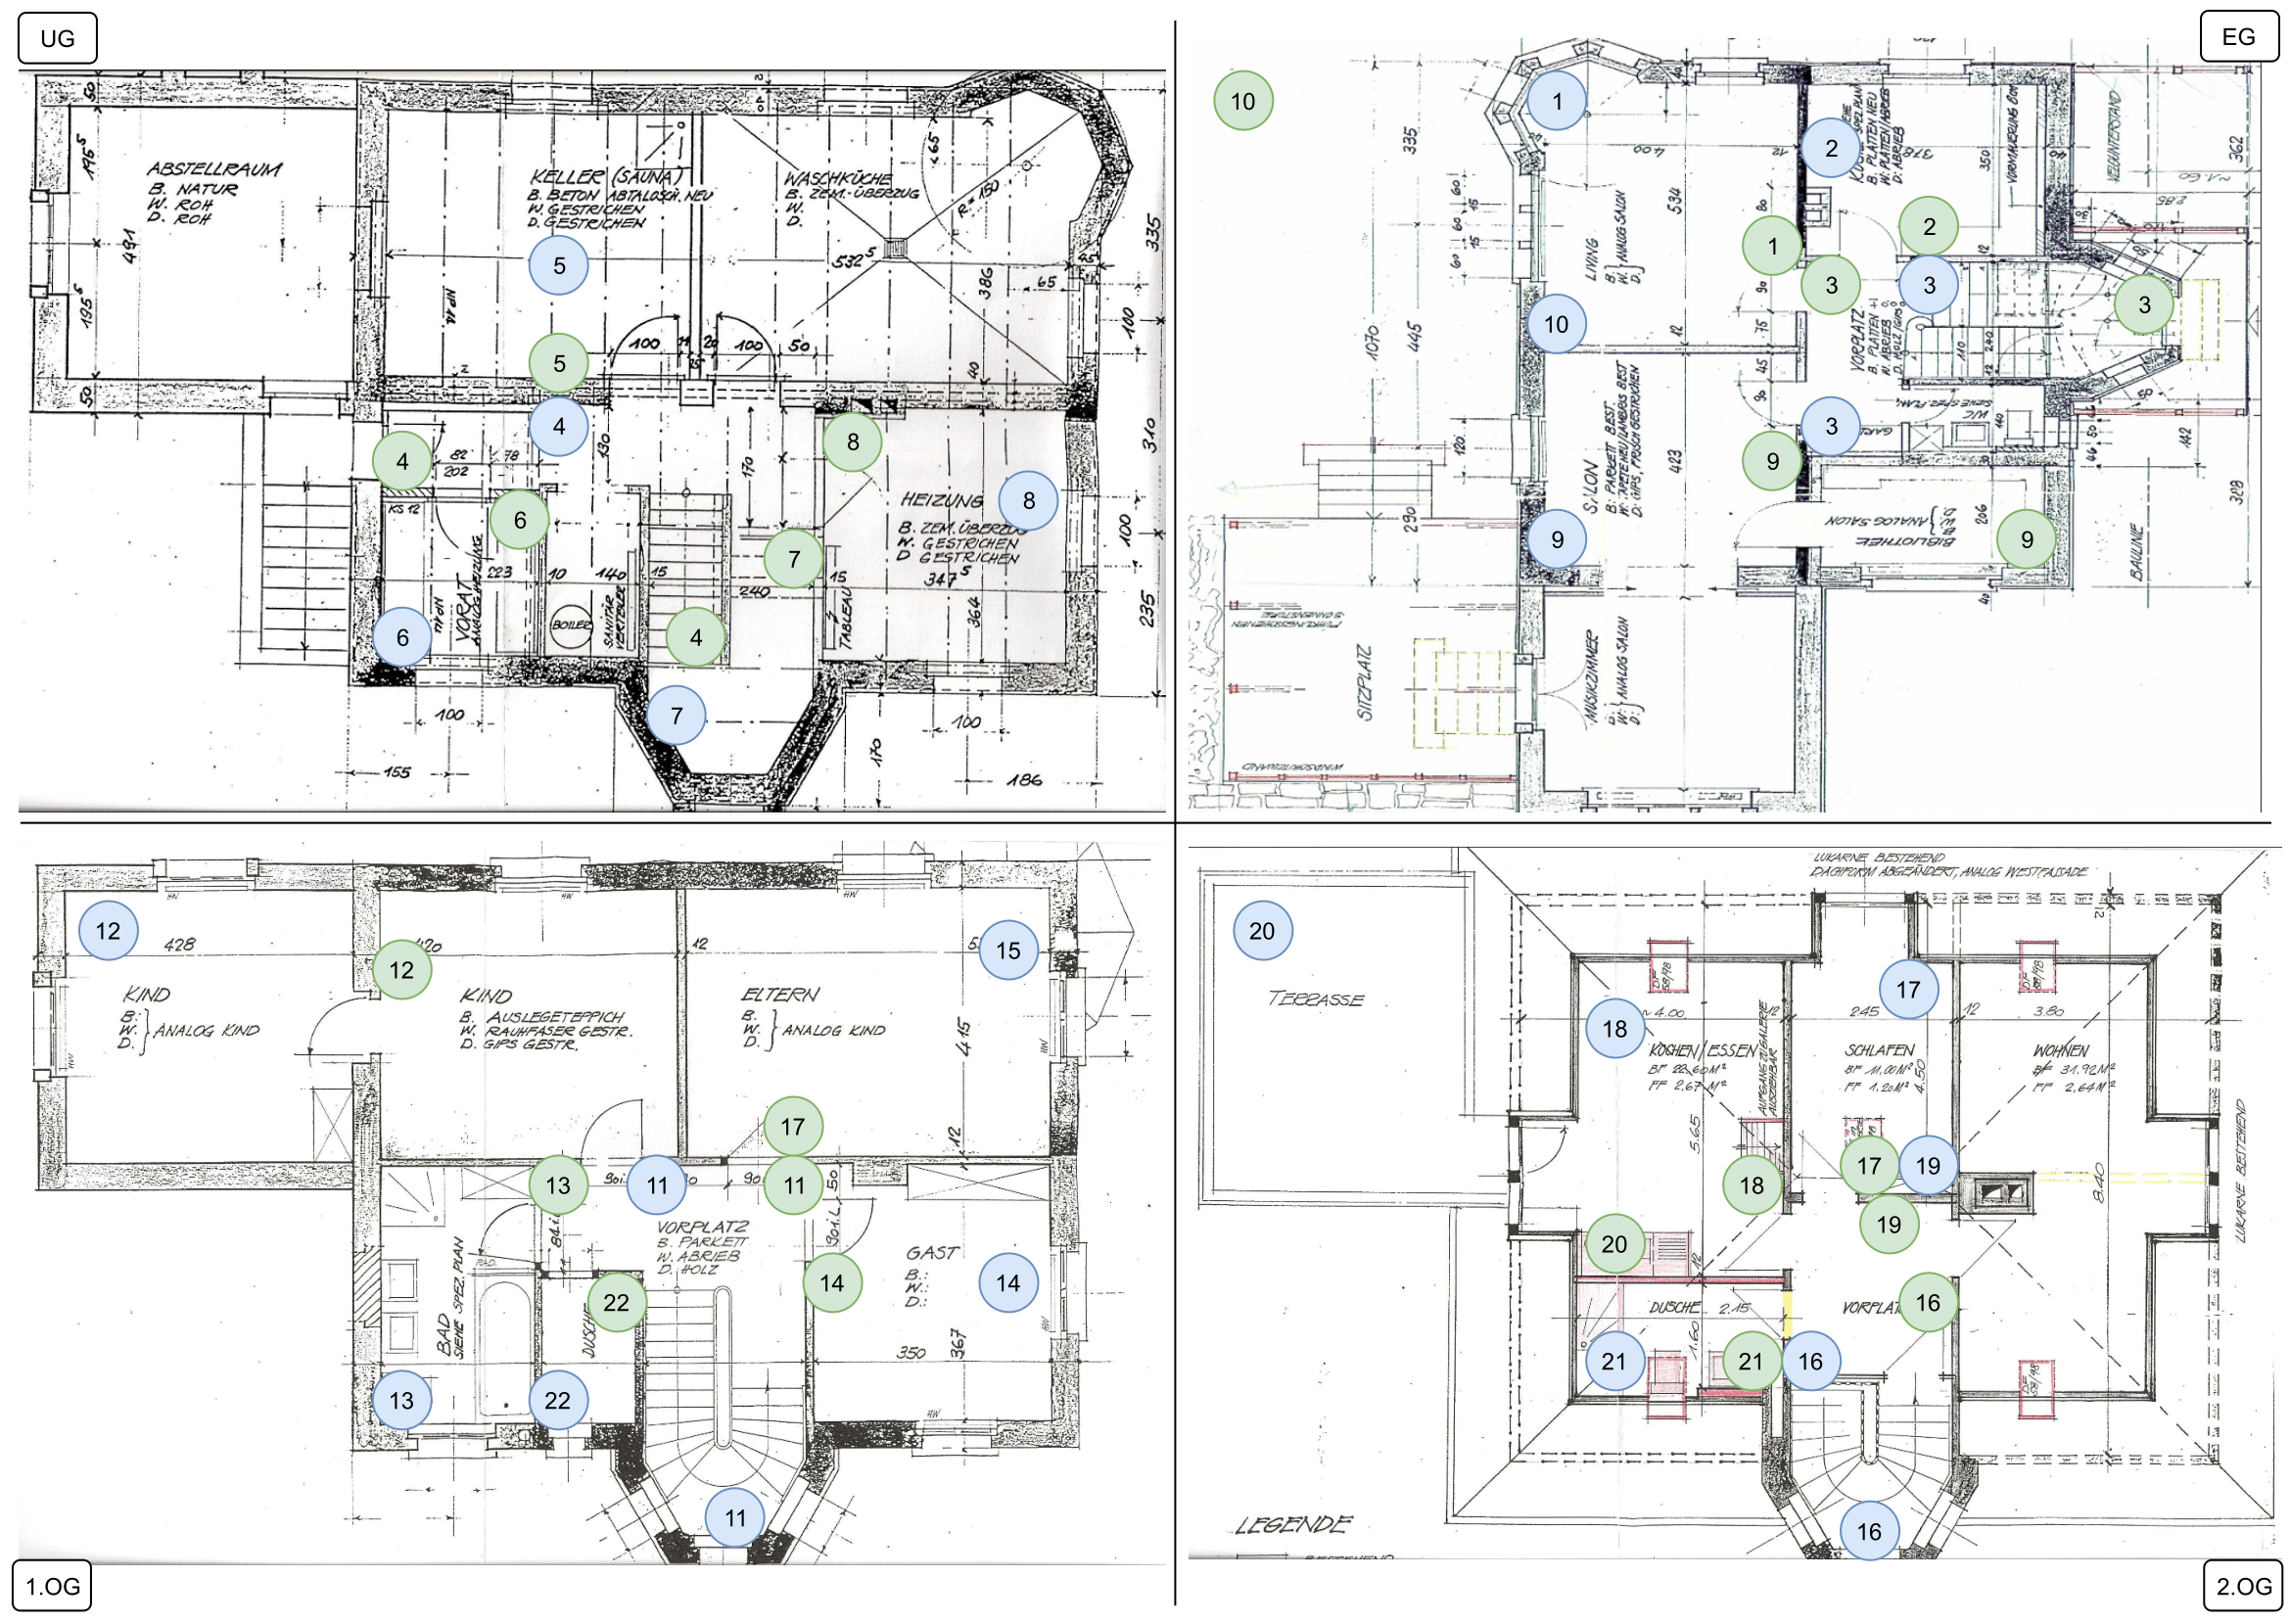
\includegraphics[width=\textwidth]{Plan_Haus_Raffi.png}
	\caption{Platzierung der Nodes im Einfamilienhaus}\label{fig:Messumgebung2Einfamilienhaus}
\end{figure}
	
\paragraph{Wohnung}
Ebenfalls als Heim-Automatisierung gedacht werden die Messungen in einer Wohnung durchgeführt.
\begin{itemize}
	\item Wohnung über eine Etage in einem Mehrfamilienhaus
	\item Anzahl Sensoren und Aktoren vergleichbar gross.
	\item Node-Dichte höher als im Haus.
	\item Mögliche Störeinflüsse durch andere Systeme von Nachbarn sind zu erwarten.
	\item Sämtliche Mesh-Beziehungen gemäss \ref{subsubsec:MeshBeziehungen} kommen vor und werden durch die bestehende Infrastruktur bestimmt.
\end{itemize}

Bei der Wohnung handelt es sich um eine 3.5 Zimmer Wohnung mit einer Wohnfläche von 122 Quadratmetern. Die genauen Abmessungen sowie die Platzierung der Nodes ist in Abbildung \ref{fig:PlatzierungderNodesinMessumgebung3} zu sehen.

\begin{figure}[H]
	\centering
	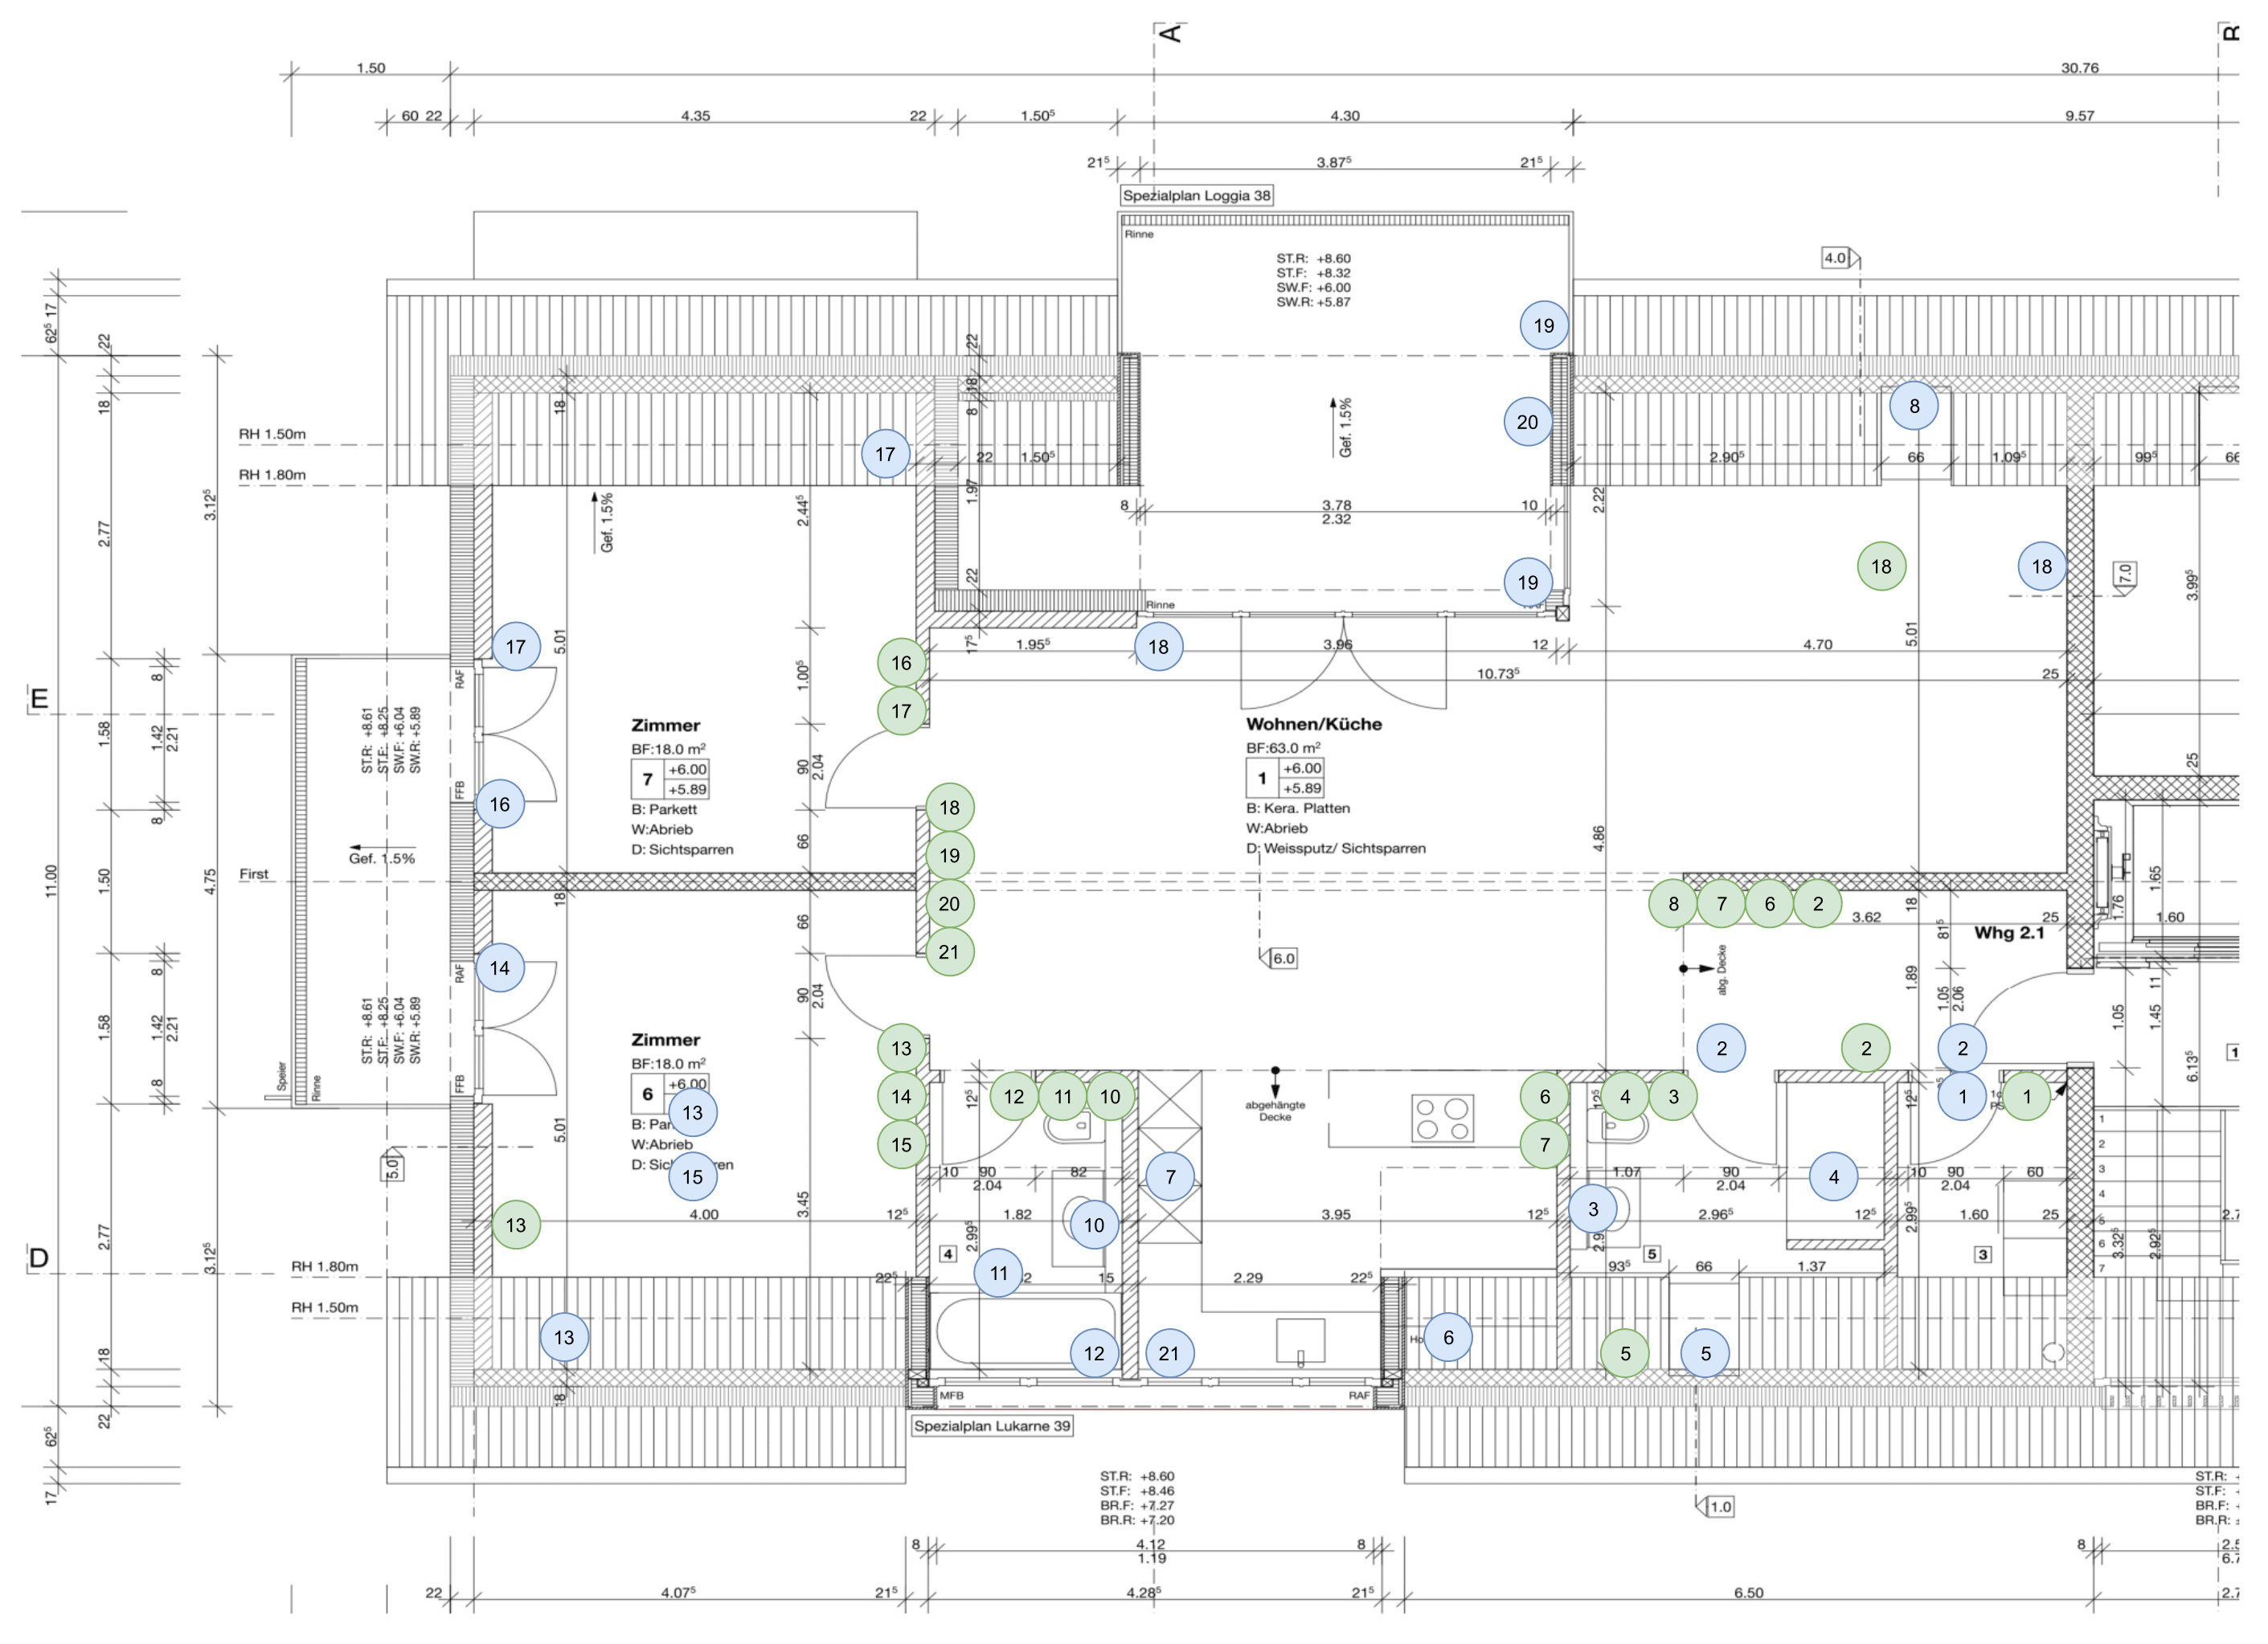
\includegraphics[width=\textwidth]{Plan_Wohnung_Cyrill_Nodes_Placement.png}
	\caption{Platzierung der Nodes in Messumgebung 3 (Wohnung)}\label{fig:PlatzierungderNodesinMessumgebung3}
\end{figure}




\subsection{Ablauf}\label{subsec:AblaufMesh}

Ein Mesh Benchmark folgt einem klar definierten Ablauf. Die Abbildung \ref{fig:MeshTestKonzept} zeigt das Testkonzept in welchem auch der Ablauf eines Benchmarks bereits angedeutet ist.

\begin{enumerate}
	\item \textbf{Benchmark User-Init:}\\
	Im Config File auf dem BMS werden die gewünschten Parameter definiert, die Konfiguration verteilt und der Benchmark durch den Benutzer gestartet.
	\item \textbf{Benchmark Init BMN:}\\
	Die Parameter werden an den BMN übergeben welcher diese wiederum an alle teilnehmenden BSN weiterleitet. Mit einem Startsignal vom BMN wird der Benchmark auf den BSN gestartet.
	\item \textbf{Benchmark Prozess:}\\
	Die BSN führen den Benchmark Prozess mit den definierten Parametern aus. Dies geschieht autonom und jeweils nur zwischen den entsprechenden BSN die gemäss Benutzerkonfiguration in einer direkten Beziehung zueinander stehen (siehe Mesh Beziehungen \ref{subsubsec:MeshBeziehungen}). Die entstandenen Messdaten werden auf den BSN zwischengespeichert und nach Ablauf des Benchmarks ins Flash geschrieben.
	\item \textbf{Reporting:}\\
	Nach Ablauf der Benchmark Zeit werden die Messdaten an den BMN übertragen. Dies erfolgt gesteuert durch den BMN welcher die Daten bei einem BSN nach dem anderen abfragt und direkt an das BMS weiterleitet.
	\item \textbf{Finish:}\\
	Der BMN kontrolliert ob er die Daten von sämtlichen BSN korrekt auslesen konnte und bestätigt das Ende der Messung gegenüber dem BMS.
	\item \textbf{Auswertung:}\\
	Das BMS beendet den Benchmark Vorgang, speichert die Messdaten in seiner Datenbank ab und bereitet diese grafisch auf. 
\end{enumerate}

%\subsection{Anforderungen}\label{subsec:SoftwareAnforderungen}
%\todo[inline]{Titel ändern. Und Text an restliches Kapitel anpassen.}
%Wie bereits im Abschnitt \ref{sec:Abgrenzung} wurden die Anforderungen in der Aufgabenstellung (siehe Anhang \ref{app:Aufgabenstellung}) sowie im Pflichtenheft (siehe Anhang \ref{app:Pflichtenheft}) vorgängig festgelegt. Im Fokus steht das erfassen der wichtigsten Messgrössen welche nachfolgend aufgeführt werden.
%
%\begin{itemize}
%	\item \textbf{Latenzzeit}: Bestimmung der Latenzzeit in Millisekunden zwischen den Teilnehmern. Die Genauigkeit sollte bei $+/-$1 ms liegen.  
%	\item \textbf{Anzahl Hops}: Bestimmung der Anzahl Hops, über welche eine Nachricht übermittelt wird.
%	\item \textbf{Datenrate}: Messen der Datenrate in Bytes/s, welche zwischen zwei Teilnehmern erreicht wurde. 
%	\item \textbf{RSSI}: Erfassen des RSSI-Werts der eingehenden Pakete.
%	\item \textbf{Paketverlust}: Pakete zählen, welche ihr Ziel nicht erreicht haben.  
%	\item \textbf{Aktive Radio Zeit}: Erfassen der aktiven Radio-Zeit um den Energieverbrauch abschätzen zu können. 
%\end{itemize}
%
%
%Die Erfassung muss in allen Mesh-Netzwerken möglich sein. Um die Messresultate vergleichen zu können müssen die gleichen Ausgangslagen vorliegen, sowie die selben Messmethoden angewendet werden. 



\subsection{Vergleichswerte und Messgrössen}\label{subsec:VergleichswerteundMessgrössenMesh}
Beim Vergleich der Mesh Protokolle wird zwischen Vergleichswerten und Messgrössen unterschieden. Vergleichswerte sind meist aus einer oder mehreren Messgrössen berechnete Werte die einen aussagekräftigen Vergleich ermöglichen.

\subsubsection{Vergleichswerte}\label{subsubsec:Vergleichswerte}
Im Pflichtenheft zu dieser Arbeit (Anhang \ref{app:Pflichtenheft}) wurden die Testkriterien für den Vergleich bereits ausführlich behandelt.
Folgende Vergleichswerte kommen nun in der Auswertung effektiv zum Tragen:

\begin{itemize}
	\item \textbf{Latenzzeit}: Bestimmung der Latenzzeit in Millisekunden eines Pakets das über das Mesh vom Client zum Server versendet wird.  
	\item \textbf{Anzahl Hops}: Bestimmung der Anzahl Hops, über welche eine Nachricht übermittelt wird.
	\item \textbf{Datenrate}: Messen der Datenrate in Bytes/s, welche zwischen zwei Teilnehmern erreicht wurde. 
%	\item \textbf{RSSI}: Erfassen des RSSI-Werts der eingehenden Pakete.
	\item \textbf{Paketverlust}: Pakete welche ihr Ziel nicht erreichen konnten werden gezählt um so eine Paketverlustrate zu ermitteln.
	\item \textbf{Aktive Radio Zeit}: Zur Abschätzung des Energieverbrauchs der Nodes im Mesh Betrieb, wird die Aktivdauer der Radio Schnittstelle gemessen.
\end{itemize}


\subsubsection{Messgrössen}\label{subsubsec:Messgrössen}

Um diese Werte zu erfassen sind spezifische Messgrössen gefragt die auf den Nodes direkt erfasst werden können.
Die untenstehende Auflistung zeigt die auf den Mesh Nodes erfassten Messgrössen, deren Generierung und wie diese in der Auswertung verwendet werden.


\paragraph{Message Timestamp}
Zur Bestimmung der Latenzzeit eines Pakets das über das Mesh Netzwerk versendet wird, wird beim Senden sowie beim Empfangen ein Message Timestamp erfasst.
Die unter den Nodes synchronisierte Zeit gibt Aufschluss darüber wie lange das Paket unterwegs war. Die Berechnung der Latenzzeit wird jedoch erst bei der Analyse auf dem BMS durchgeführt.

\paragraph{Number of Hops}
Die oben erwähnte Latenzzeit ist in einem Mesh Netzwerk abhängig vom Weg den ein Paket bei der Übermittlung genommen hat. Mit jedem Hop nimmt die Latenzzeit zu.
Deshalb wird beim Server Node die Anzahl Hops die das Paket genommen hat aus dem Message Header ausgelesen und für die Bestimmung der Latenzzeit abgespeichert.

\paragraph{Source-, Destination-, Group-Address}
Aufgrund der veränderlichen Beziehungen von Client und Server Nodes ist die Zuordnung von Quell- und Zieladresse eines Pakets ebenfalls nicht statisch. Aus diesem Grund werden auf allen Nodes die Quell-, Ziel- und Gruppenadressen der Pakete ausgelesen. 
Somit kann das Benchmark Paket eindeutig identifiziert und in der Auswertung erfasst werden.
Die Adressinformationen werden aus dem Message Header des Mesh Pakets ausgelesen oder im Falle des Client Nodes mit der Benchmark Control Message übermittelt.

\paragraph{Message ID}
Als Payload im Mesh Paket versendet, identifiziert die Message ID das Paket zusammen mit den Adressinformationen eindeutig. So kann Paketverlust wie auch die Latenzzeit erfasst werden.

\paragraph{RSSI}
Der RSSI (Received Signal Strength Indication) wird auf dem Server Node auf MAC Ebene erfasst und zeigt die Empfangsstärke zum zuletzt passierten Hop. Dies gibt Aufschluss über die Empfangsqualität und kann bei der Analyse des Benchmarks als weiterer Indikator für Paketverlust und Latenzzeit verwendet werden.

\paragraph{Aktive Radio Zeit}
Die Zeit in der die Radio Schnittstelle aktiv ist wird auf dem Node direkt gestoppt und gespeichert.


\subsection{Messreihe}\label{subsec:Messreihe}
Um die Mesh Protokolle einem möglichst fairen Vergleich zu unterziehen, werden pro Testumgebung eine Reihe an Messungen durchgeführt. Die Tabelle \ref{tab:ParameterBenchmarkMessreihe} zeigt Total 8 Messreihen mit den entsprechenden Parametern.

Die Messungen 1 bis 5 werden in allen drei Messaufbauten durchgeführt. So werden die Unterschiede der Topologien ersichtlich.
Die Messungen 6 bis 8 hingegen werden nur im Laboraufbau durchgeführt damit allfällige Externe Störeinflüsse ausgeschlossen werden können und das Mesh Netzwerk unter Extrembedingungen getestet werden kann.

Bei der Messung mit dem Index 6 handelt es sich um ein Benchmark welcher mit der P2P Testinfrastruktur gestört wird. So soll die Störimmunität des Mesh Stacks getestet werden.
Die Messungen 7 und 8 wurden aufgrund der Erfahrungen die mit den Resultaten der Messungen 1 bis 6 gesammelt werden konnten, nachträglich ergänzt. In Abschnitt \ref{sec:Validierung} wird genauer auf diese Problematik eingegangen.
Die Dichte der Nachrichten ist bei diesen Messungen deutlich tiefer.


\begin{table}[h]
\centering
\begin{adjustbox}{width=1\textwidth}
\begin{tabular}{|c|c|c|c|c|c|c|c|c|} 
\cline{2-9}
\multicolumn{1}{c|}{} & \multicolumn{5}{c|}{Benchmark Parameter} & \multicolumn{3}{c|}{Messaufbau} \\ 
\hline
\textbf{\#}  & \textbf{Msg. Gen.}  & \textbf{Duration} & \textbf{Msg. Cnt.}  & \textbf{Payload }  & \textbf{Disturbance}  & \textbf{Labor}  & \textbf{Haus}  & \textbf{Wohnung}  \\ 
\hline
1 & Rand & 600s & 60 & Small & No & x & x & x \\ 
\hline
2 & Seq & 600s & 60 & Small & No & x & x & x \\ 
\hline
3 & Rand & 600s & 60 & Large & No & x & x & x \\ 
\hline
4 & Seq & 600s & 60 & Large & No & x & x & x \\ 
\hline
5 & Rand & 600s & 600 & Small & No & x & x & x \\ 
\hline
\multicolumn{1}{c}{} & \multicolumn{1}{c}{} & \multicolumn{1}{c}{} & \multicolumn{1}{c}{} & \multicolumn{1}{c}{} & \multicolumn{1}{c}{} & \multicolumn{1}{c}{} & \multicolumn{1}{c}{} & \multicolumn{1}{c}{} \\ 
\hline
6 & Rand & 600s & 60 & Small & Yes & x &  &  \\ 
\hline
7 & Seq & 750s & 10 & Small & No & x &  &  \\ 
\hline
8 & Seq & 750s & 10 & Large & No & x &  &  \\
\hline
\end{tabular}
\end{adjustbox}
\caption{Parameter Benchmark Messreihe}
\label{tab:ParameterBenchmarkMessreihe}
\end{table}

Die Erläuterungen über die Bedeutung der Parameter ist in der folgenden Tabelle \ref{tab:BedeutungBenchmarkParameter} zu finden. 

\begin{table}[h]
\centering
\begin{adjustbox}{width=1\textwidth}
\begin{tabular}{lll} 
\toprule
Parameter: & Gültige Werte: & Bedeutung: \\ 
\hline
Msg. Gen & Seq/Rand & Nachrichten Generierung Sequentiell oder Pseudozufällig \ref{subsec:TrafficGeneration}. \\
Duration & Ganze Zahlen & Dauer eines Benchmarks angegeben in Sekunden. \\
Msg. Count & Ganze Zahlen & Anzahl der Nachrichten die pro Client Node versendet werden.\\
Payload & Small/Large & Grosse oder Kleine Payload gemäss Definition in Tabelle.\\
Disturbance & Yes/No & \begin{tabular}[t]{@{}l@{}}Gewollte Störung durch P2P Testinfrastruktur auf\\dem selben Channel. \end{tabular} \\
\bottomrule
\end{tabular}
\end{adjustbox}
\caption{Bedeutung Benchmark Parameter}
\label{tab:BedeutungBenchmarkParameter}
\end{table}


\subsection{Allgemeine Benchmark Parameter}\label{subsec:AllgemeineBenchmarkParameter}

Die oben erwähnten Messreihen haben nebst den variablen Parametern einige allgemeingültige Benchmark Parameter die in der Tabelle \ref{tab:AllgemeineBenchmarkParameter} aufgeführt sind.
Diese sind für sämtliche Messungen innerhalb des jeweiligen Mesh Protokolls gültig.
In den Punkten \textit{Message Ack, Mesh Node Cnt., Client/Server Verhältnis}, sowie \textit{Payload Size Small} unterscheiden sich die Benchmarks der drei Protokolle nicht.
Die Benchmark Nachrichten werden auf dem Application Layer \textit{unacknowledged} versendet. Wenn also ein Paket sein Ziel nicht erreicht, wird dies vom Sender nicht registriert und das Paket nicht erneut übertragen.
Sämtliche Benchmarks werden mit 50 Mesh Nodes durchgeführt. Davon sind jeweils gleich viele Client Nodes wie Server Nodes \ref{subsubsec:Nodes}.

\begin{table}[h]
\centering
\begin{adjustbox}{width=1\textwidth}
\begin{tabular}{lccc} 
\toprule
 & BT Mesh & Thread & Zigbee \\ 
\hline
Group addressing mode & Broadcast & Multicast & Unicast \\
Application Layer & Models & CoAP & ZCL (Zigbee Cluster Library) \\
MAC-Layer & BLE 1M & IEEE 802.15.4 & IEEE 802.15.4 \\
Mesh Node Type & Relay & FTD (Full Thread Device) & Zigbee-Router \\
Mesh Node Cnt. & 50 & 50 & 50 \\
Client/Server Verhältnis & 25/25 & 25/25 & 25/25 \\
Message Ack (Appl. Layer) & No & No & No \\
Payload Size Small (Byte) & 8 & 8 & 8 \\
Payload Size Large (Byte) & 32 & 50 & 50 \\
\bottomrule
\end{tabular}
\end{adjustbox}
\caption{Allgemeine Benchmark Parameter}
\label{tab:AllgemeineBenchmarkParameter}
\end{table}

Die Parameter \textit{Group addressing mode} sowie \textit{Payload Size Large} unterscheiden sich aufgrund der Eigenschaften der Protokolle leicht.
Beim \textit{Group addressing mode} wird zwischen Broadcast bei BT Mesh, Multicast bei Thread und Unicast bei Zigbee unterschieden. Gemäss Definition im Pflichtenheft soll jeweils eine Gruppenadressierung stattfinden. Zigbee bietet zwar eine solche Möglichkeit eines Multicasts jedoch wird dieser schliesslich als Broadcast umgesetzt was eine deutliche Limitierung der Performance verursacht.
Aufgrund dieser Erfahrung und der Erkenntnis dass marktübliche Lichtsteuerungen\footnote{Analyse mittels Sniffer Trace einer IKEA Tradfri Lichtsteuerung.} nur selten ein solches Multicast Prinzip verwenden, wird die Adressierung im Benchmark gerichtet (Unicast) vorgenommen (siehe auch \ref{sec:ZigbeeUmsetzungBenchmark}).
Das bedeutet die Nachrichten werden nicht an eine Gruppenadresse sondern direkt an die jeweilige Node Adresse gesendet. Bei mehreren Servern innerhalb einer Gruppe werden also auch mehrere Nachrichten versendet.

Die \textit{Payload Size Large} soll eine vergleichsweise grosse Payload simulieren die über das Mesh übertragen wird.
Die beiden Protokollstacks Thread und Zigbee erlauben dank IEEE 802.15.4 beide eine totale Framegrösse von 127 Byte.
Abzüglich der Grösse der Header bieten die Protokolle noch Platz für eine Payload von ca. 50 Byte. Je nach Implementation der Protokolle variiert die Header Grösse und die Payload kann entsprechend erhöht werden.
BT Mesh hingegen beginnt bereits bei einer Payload Grösse von 8 Byte mit der Fragmentierung. Somit werden bei den 32 Byte für die \textit{Payload Size Large} bereits 4 Frames versendet. Diverse Tests haben ergeben, dass hier der BT Mesh Stack an seine Leistungsgrenze stösst.
Aus diesem Grund ist eine weitere Erhöhung der Payload nicht sinnvoll.


\subsection{Traffic Generation}\label{subsec:TrafficGeneration}

Die in Tabelle \ref{tab:BedeutungBenchmarkParameter} erwähnte Message Generation ist im Benchmark verantwortlich für die Verteilung der Benchmark Nachrichten über die Nodes in Abhängigkeit der Zeit. So wird bestimmt wie der Traffic innerhalb des Netzes sowie auf den einzelnen Nodes generiert wird.
Dabei werden die folgenden zwei Modi unterschieden:

\paragraph{Random}\label{par:Random}
Im Modus \textit{Random} werden die Zeitpunkte für den Versand einer Nachricht sogenannt pseudozufällig generiert. Dies bedeutet, dass jedem Client Node eine Liste von einmalig zufällig generierten Werten zugewiesen wird.
Aus dieser Liste werden nur so viele Werte gelesen wie es Nachrichten zu versenden gilt. Diese werden schliesslich nach Grösse sortiert und über den gesamten Benchmark Zeitraum gelegt woraus nun die Zeitpunkte für den Versand der Nachrichten entstehen.
Ein solche Methode erlaubt es die Zeitpunkte reproduzierbar zu machen und identisch auf alle 3 Mesh Stacks anzuwenden.

\paragraph{Sequentiell}\label{par:Sequentiell}
Mit der \textit{Random} Methode kann die Belastung eines Nodes sowie des gesamten Netzes zwischenzeitlich stark ansteigen.
Um dies zu verhindern, kann der Traffic Generation Modus \textit{Sequentiell} gewählt werden.
Dabei werden die Nachrichten in regelmässigen Zeitschlitzen gemäss \ref{eq:TrafficGenerationSeq} pro Node versendet. Die Reihenfolge der Nodes bleibt jeweils die selbe.


\begin{equation}\label{eq:TrafficGenerationSeq}
T_{Msg\_send} =  \frac{T_{Bench\_Duration}}{(Msg\_Cnt \cdot 25)} \cdot NodeID \cdot i_{Msg}
\end{equation}

\begin{small}
\begin{center}
\begin{tabular}{ll}
$T_{Msg\_send}$ & Zeitpunkt zu welchem die Nachricht gesendet wird.\\
$T_{Bench\_Duration}$ & Benchmark Dauer (siehe \ref{tab:ParameterBenchmarkMessreihe})\\
$Msg\_Cnt$ & Anzahl Nachrichten die versendet werden.\\
$NodeID$ &Identifikationsnummer des Nodes. \\
$i_{Msg}$ & Message Index
\end{tabular}
\end{center}
\end{small}





\subsection{Messdatenerfassung und Auswertung}\label{subsec:MessdatenerfassungundAuswertung}

Für die Messdatenerfassung und Auswertung wird keine dedizierte Hardware verwendet. Die eigentlichen Messwerte die in Abschnitt \ref{subsec:VergleichswerteundMessgrössenMesh} erläutert sind, werden auf den Mesh Nodes direkt erfasst und erst im RAM und später im Flash des Microcontrollers zwischen gespeichert. Von dort werden sie mittels BRM (Benchmark Report Message) an den BMN übertragen.
Auf den Mesh Nodes inkl. BMN findet noch keine Auswertung der Daten statt.
Diese wird an das BMS ausgelagert.
Das BMS empfängt die BRM via CLI (Command Line Interface) und speichert die Messwerte in einem Excel CSV File ab. Dazu kommt ein Python Skript zum Einsatz (siehe \ref{subsubsec:Benchmark}).
Mittels einem weiteren Python Skript und manueller Bearbeitung in Excel können die so erfassten Daten ausgewertet werden.


\subsubsection{Identifizierung der Teilnehmer}\label{subsubsec:NodeIdentification}

\todo[inline]{Raffi: Kurze Beschreibung wie die 50 Nodes auseinander gehalten werden. (MAC-Address-LSB). Bei Dongle mit Bild wo die MAC-Adresse abzulessen ist. Hinweis zur erfassung in der Excel-Liste zur Konfiguration. Hinweis das die MAC-Addresse zufällig generiert, jedoch fix in jedem DOngle eingebrant ist (FICR--REgister). }

\subsubsection{Konfiguration der Teilnehmer}\label{subsubsec:NodeConfiguration}

\todo[inline]{Raffi: Kurze Beschreibung wie die 50 Nodes Konfigueriert werden können (über einfache CLI Befehle). Alle Felder kurz mit ihrer Bedeutung auf das Benchmark KOnzept beschreiben (Group-ID = Gruppe, DST\_MAC\_1 = Zigbee Direct Addressing... etc.. setNodeSettings <MAC in Integer format> <GroupNumber> <Node Id> <Ack> <AdditionalPayloadSize> <BenchmarkTrafficGenMode> <DST\_MAC\_1> <DST\_MAC\_2> <DST\_MAC\_3>}


\subsubsection{Starten einer Messung}\label{subsubsec:StartofMeassurment}

\todo[inline]{Raffi: Kurze Beschreibung wie eine Messung gestartet wird und was die Beidern Fleder im Bfehl Bedeuten (verweis auf obiges KOnzept)}

\subsubsection{Einholen der Messdaten}\label{subsec:NodeConfiguration}

\todo[inline]{Raffi: Kurze Beschreibung wie eine das Reporting eingeleitet wird. Viele Detail ssind dazu ubereits im Software Teil vorhanden. }


\subsection{Messerwartung}\label{subsec:Messerwartung}
Wie in der Übersicht \ref{subsec:VorarbeitenP5} bereits erwähnt, konnte im Rahmen der Vorarbeiten zu dieser Thesis der BT Mesh Stack bereits vertieft untersucht und erste Erfahrungen damit gesammelt werden. Bei den beiden anderen Stacks, Thread und Zigbee musste dies erst noch erfolgen.
Bei eben diesen Vorarbeiten konnten bereits deutliche Unterschiede zwischen den Stacks beobachtet werden, hauptsächlich verursacht durch das Routing bei Thread und Zigbee sowieso das Flooding-Mesh bei BT Mesh.
Aufgrund dieser Erfahrungen wird erwartet, dass die beiden auf dem IEEE 802.15.4 Standard aufbauenden Protokolle klare Vorteile haben werden da die Nachrichtenzustellung durch das Routing effizienter realisiert werden kann.


\todo[inline]{Cyrill: Welche Resultate werden erwartet. Welcher der drei Stacks ist vermeintlich der Beste?}

\pagebreak

\clearpage
\section{Hardware Plattform}\label{sec:HardwarePlattform}
\todo[inline]{Cyrill}

\todo[inline]{Übersicht über die eingesetzte Hardware. Einleitung inkl. Erläuterung Unterschiede und Gemeinsamkeiten P2P und Mesh Test Hardware (Stichwort: Open Source, Open Hardware).}

Für den Benchmark und den Vergleich der drei Mesh Protokolle sowie die P2P Testinfrastruktur wird eine einheitliche Hardwareplattform verwendet. Dies macht ein Vergleich der Testresultate möglich. Im Zentrum steht dabei der nRF52840 SoC von Nordic Semiconductor welcher eine voll umfängliche Plattform für Bluetooth und IEEE 802.15.4 darstellt. Damit besonders die P2P Testinfrastruktur einfach nutzbar ist, werden Entwicklungsboards vom Chip Hersteller eingesetzt welche vergleichsweise günstig und gut verfügbar sind. Nachfolgend wird auf die Hardware und deren Einsatz genauer eingegangen.


\subsection{System on Chip}\label{subsec:SystemonChip}

Der nRF52840 ist ein Highend System-on-Chip welcher gleichermassen Bluetooth 5 wie auch den IEEE 802.15.4 Wireless-Personal-Area-Network (WPAN) Standard unterstützt. Auf Wunsch sogar als Multiprotocol Lösung.
Entscheidend für die vorliegende Anwendung ist, dass der SoC von den drei Organisationen Bluetooth SIG, Openthread und der Zigbee Alliance offiziell für das jeweilige Protokoll zertifiziert ist.
Die Eckdaten des nRF52840 SoC sind in der Tabelle \ref{tab:EigenschaftennRF52840SoC} kurz zusammengefasst.

\begin{table}[h]
\centering
\begin{tabular}{ll}
\toprule
Microcontroller    & 32-bit ARM Cortex-M4F                        \\
Clock frequency    & 64 MHz                                       \\
Flash              & 1MB                                        \\
RAM                & 256kB                                          \\
Frequency Band     & 2.4GHz                                       \\
Wireless protocols & IEEE 802.15.4 (Thread, Zigbee), Bluetooth 5.0  \\
\bottomrule
\end{tabular}
\caption{Eigenschaften nRF52840 SoC \cite{nordic_semiconductor_asa_nrf52840_2020}}
\label{tab:EigenschaftennRF52840SoC}
\end{table}


\subsection{Hardware Development Kits}\label{subsec:HardwareDevelopmentKits}

Der Hersteller Nordic Semiconductor bietet gleich zwei Entwicklungsboards für den SoC an. Einerseits das umfangreiche nRF52840-DK (pca10056) \ref{fig:nrf52840-DK} welches zusammen mit dem Software Development Kit von Nordic Semiconductor eine vollumfängliche Entwicklungsumgebung bietet.
Auf dem Board ist nebst diverser Peripherie auch ein Segger J-Link Debugger integriert.
Dieser erleichtert das flashen und debuggen ungemein.
Im Benchmark Betrieb fungiert ein nRF52840-DK als Benchmark Master Node \ref{subsubsec:Nodes} wobei die USB-UART Schnittstelle als Interface zur Benchmark Management Station verwendet wird.
Als einfachere Alternative zum voll umfänglichen Development Kit werden als Benchmark Slave Nodes \ref{subsubsec:Nodes} die einfacheren und günstigeren nRF52840-Dongle (pca10059) \ref{fig:nrf52840-Dongle} verwendet.
Offensichtlich als USB-Dongle entworfen können die Dongles flexibel eingesetzt werden. Die fehlende Peripherie macht die Hardware jedoch unpassend für die Entwicklung neuer Firmware.
Beide Typen von Entwicklungsboards besitzen eine integrierte PCB Antenne wenn auch in unterschiedlichen Ausführungen.
Im Abschnitt \ref{subsec:AntenneundStrahlungscharakteristik} wird näher auf die Ausführung der Antennen und deren Strahlungscharakteristik eingegangen.


\begin{figure}[!htbp]
\centering
\begin{minipage}[b]{0.49\textwidth}
		\centering
		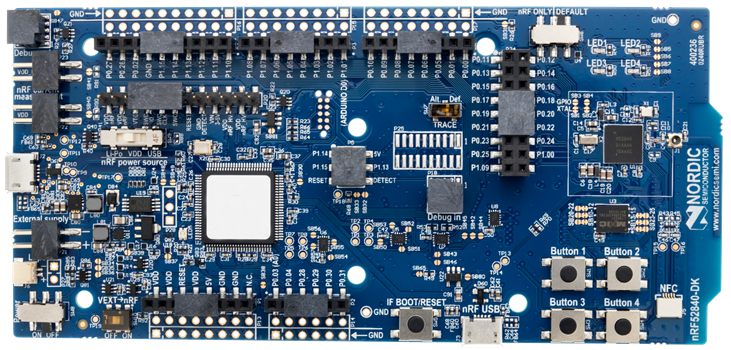
\includegraphics[width=\textwidth]{nRF52840_DK.png}
		\caption[nRF52840-DK PCA10056]{PCA10056 \cite{nordic_semiconductor_asa_nrf52840_2020-1}}
		\label{fig:nrf52840-DK}
\end{minipage}
\begin{minipage}[b]{0.49\textwidth}
		\centering
		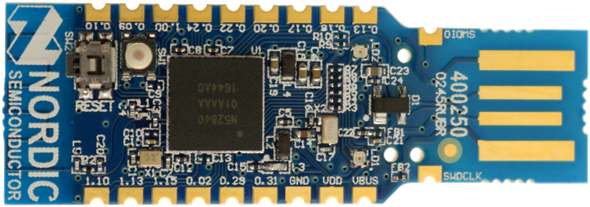
\includegraphics[width=0.9\textwidth]{nRF52840_Dongle_gerade.png}
		\caption[nRF52840-Dongle PCA10059]{PCA10059 \cite{nordic_semiconductor_asa_nrf52840_2020-2}}
		\label{fig:nrf52840-Dongle}
\end{minipage}
\end{figure}



\subsection{Aufbau Testnode}\label{subsec:AufbauTestnode}

Der Aufbau des Testnodes wie er in Abbildung \ref{fig:TestnodenRF52840-DongleinklBatteriepack} wurde so einfach wie möglich gehalten. Ein externes Batteriepaket wird eingesetzt, damit der Benchmark Slave Node unabhängig von einer externen Stromversorgung betrieben werden kann. So kann der Einsatzort frei gewählt und auch kurzfristig geändert werden.
Das Batteriepaket besteht aus zwei Standard Mignon Einwegzellen vom Typ AA mit je 1.5V Spannung. In Serieschaltung betrieben wird die Speisespannung von 3V erreicht welche für den Dongle ausreichend ist. Mit fortschreitender Entladung der Zellen sinkt die Spannung. Da der SoC einen Betriebsspannungsbereich von 1.7V bis 5.5V hat stellt die sinkende Spannung jedoch kein Problem dar.
Die Speisung des nRF52840-Dongle erfolgt über einen 2-poligen JST Header der gemäss Datenblatt xx mit dem VDD OUT und GND Anschluss verbunden ist. Am VDD OUT Anschluss ist ein Betriebsspannungsbereich von 1.8V bis 3.6V zulässig.
Das Batteriegehäuse verfügt ausserdem über einen Schalter um den Testnode nach Belieben ein- und auszuschalten.
Mit den verwendeten Batterien welche je eine Kapazität von 2000mAh besitzen, können die Nodes im Mesh Benchmark Betrieb über mehrere Tage betrieben werden.
Eine Messung des Stromverbrauches im Benchmark Betrieb hat gezeigt, dass dieser bei 3V Batteriespannung durchschnittlich 15mA beträgt. Dieser relativ hohe Wert wird einerseits verursacht durch die LED's die geschaltet werden und andererseits durch das Radio Interface welches im Leerlauf permanent im Empfangsmodus ist um allfällige Start Messages empfangen zu können. 
Dieser Verbrauch ermöglicht eine Betriebsdauer von bis zu 130 Stunden. 

Die Befestigung des Dongles am Batteriepaket erfolgte so dass die PCB Antenne welche sich am Ende des PCB's befindet möglichst frei liegt und sich dadurch die bestmöglichen Abstrahlungseigenschaften ergeben. Ein weiterer Vorteil der in Abbildung \ref{fig:TestnodenRF52840-DongleinklBatteriepack} dargestellten Montage ist die Zugänglichkeit des USB Ports. So können die Benchmark Nodes auf einfachste Arte und Weise mit einer neuen Software geflasht werden.

 
\begin{figure} [H]
	\centering
	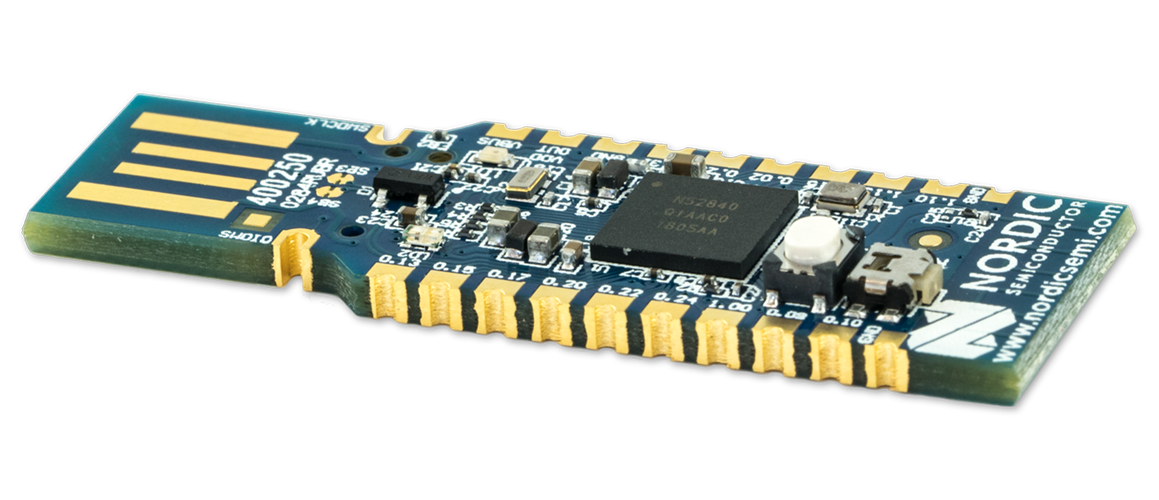
\includegraphics[width=0.4\textwidth]{nRF52840_Dongle.png}
	\caption{Testnode: nRF52840-Dongle inkl. Batteriepack}
	\label{fig:TestnodenRF52840-DongleinklBatteriepack}
\end{figure}
\todo[inline]{Bild anpassen}

\subsection{Antenne und Strahlungscharakteristik}\label{subsec:AntenneundStrahlungscharakteristik}

Wie bereits im Abschnitt \ref{subsec:HardwareDevelopmentKits} erwähnt, besitzen die beiden eingesetzten Development Kits jeweils eine PCB Antenne. Beim nRF52840-DK ist diese als einfache IFA (Inverted-F Antenna) \ref{fig:nrf52840-DK-Copper} ausgeführt während dem der Dongle mangels Platz auf dem PCB eine sogenannte MIFA (Meandered Inverted-F Antenna) \ref{fig:nrf52840-Dongle-Copper} besitzt.

\begin{figure}[!htbp]
\centering
\begin{minipage}[b]{0.49\textwidth}
		\centering
		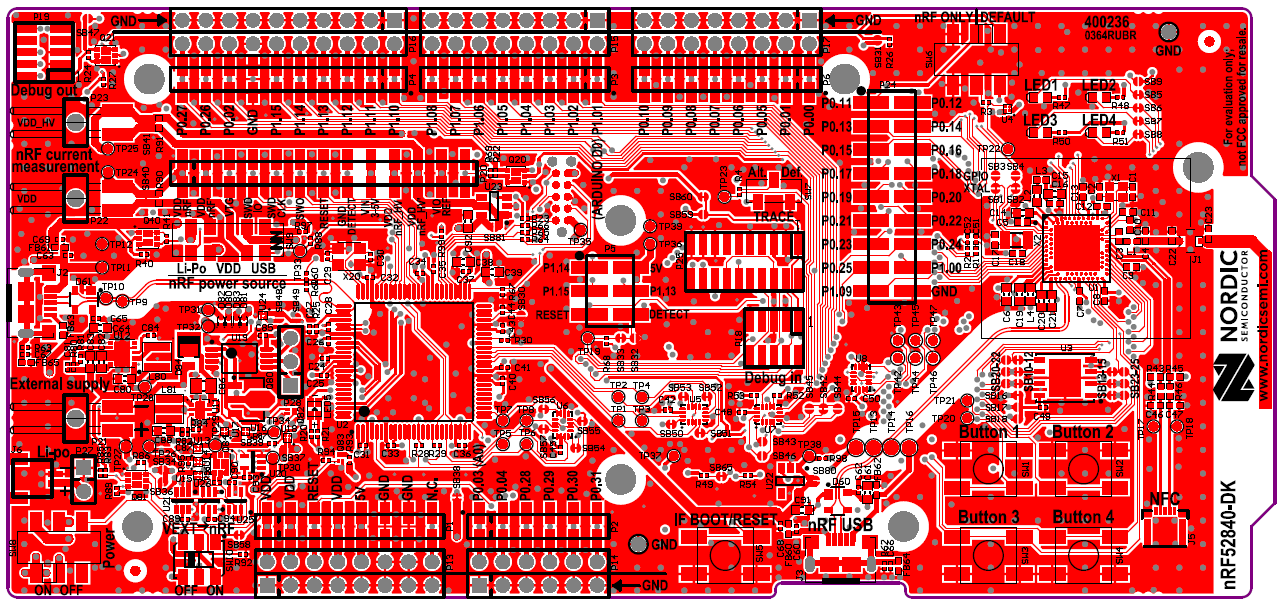
\includegraphics[width=\textwidth]{nRF52840_DK_Copper.png}
		\caption[PCA10056 Copperplane mit IFA-Antenne]{PCA10056 Copperplane \cite{nordic_semiconductor_asa_pca10056_schematic_and_pcb_2019}}
		\label{fig:nrf52840-DK-Copper}
\end{minipage}
\begin{minipage}[b]{0.49\textwidth}
		\centering
		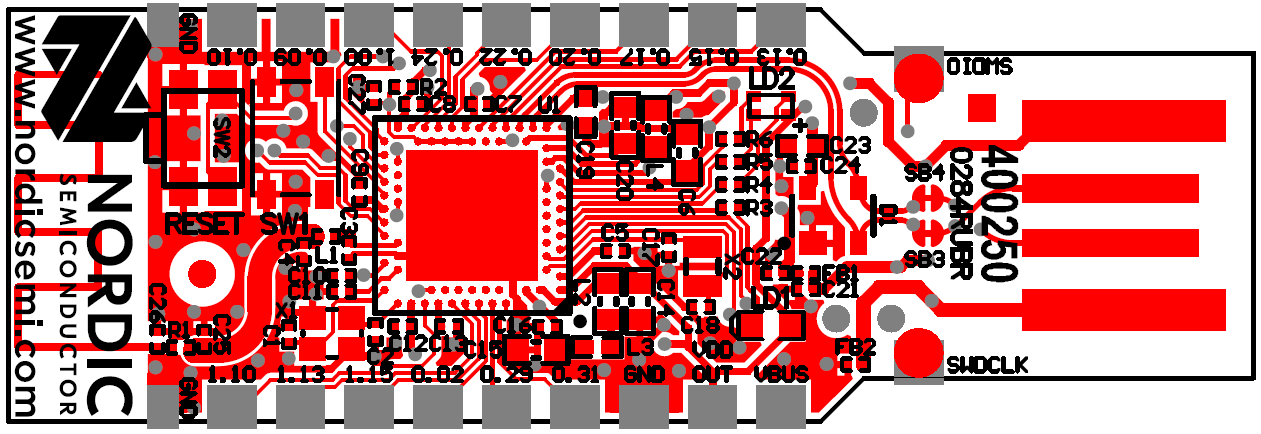
\includegraphics[width=0.9\textwidth]{nRF52840_Dongle_Copper.png}
		\caption[PCA10059 Copperplane mit MIFA-Antenne]{PCA10059 Copperplane \cite{nordic_semiconductor_asa_pca10059_schematic_and_pcb_2020}}
		\label{fig:nrf52840-Dongle-Copper}
\end{minipage}
\end{figure}

Erste Versuche zu Beginn dieser Projektarbeit haben gezeigt, dass sich die Eigenschaften der beiden Antennen relativ deutlich unterscheiden. Beispielweise konnte festgestellt werden, dass die Antenne des pca10056 eine deutlich höhere Reichweite erzielt als jene des pca10059.
Um diese Vermutungen zu prüfen wurde eine Spektrumanalyse der gestrahlten Emmission an den beiden Entwicklungsboards durchgeführt. Diese Messungen wurden im Rahmen eines Projektes für das Modul emv durchgeführt und dort in einem Bericht dokumentiert. Nachfolgend werden die wichtigsten Erkenntnisse daraus nochmals wieder gegeben. Der ganze Bericht ist im Anhang \ref{app:BerichtemvMessungDevelopmentKits} zu finden.

Bei den durchgeführten Messungen lag das Hauptaugenmerk auf der Erfassung der Abstrahlcharakteristik in dreidimensionaler Richtung. Die absoluten Signalpegel konnten dabei nicht korrekt erfasst werden, waren jedoch auch nicht von grosser Bedeutung.
Die in den beiden Abbildungen \ref{fig:PCA10056Peak} und \ref{fig:PCA10059Peak} dargestellten Abstrahlcharakteristiken der jeweiligen Development Boards zeigen deutliche Unterschiede auf. Während das pca10056 eine sehr gleichmässige Verteilung der Sendeleistung über die gesamte Halbkugeloberfläche ausweist, zeigt das pca10059 deutliche Schwachstellen in Form von Dellen in der Halbkugel auf.
Weiter unterscheidet sich der maximal Wert in Z-Richtung zwar optisch nur minimal, in Wirklichkeit bedeutet dies jedoch eine 2 bis 4 fach höhere Dämpfung und somit eine deutlich kleinere Reichweite.



\begin{figure}[!htbp]
\centering
\begin{minipage}[b]{0.49\linewidth}
	\centering
	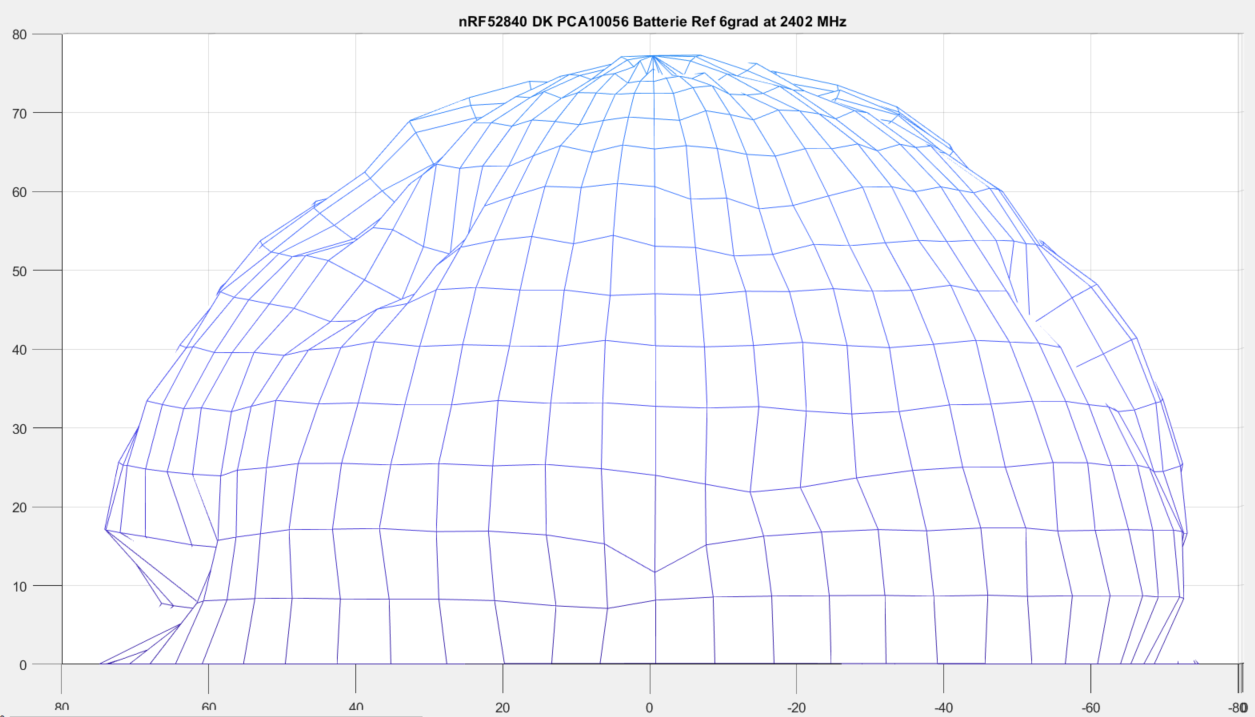
\includegraphics[width=\textwidth]{PCA10056_Peak.png}
	\caption{Abstrahlung in Z-Richtung PCA10056}
	\label{fig:PCA10056Peak}
\end{minipage}
\begin{minipage}[b]{0.49\linewidth}
	\centering
	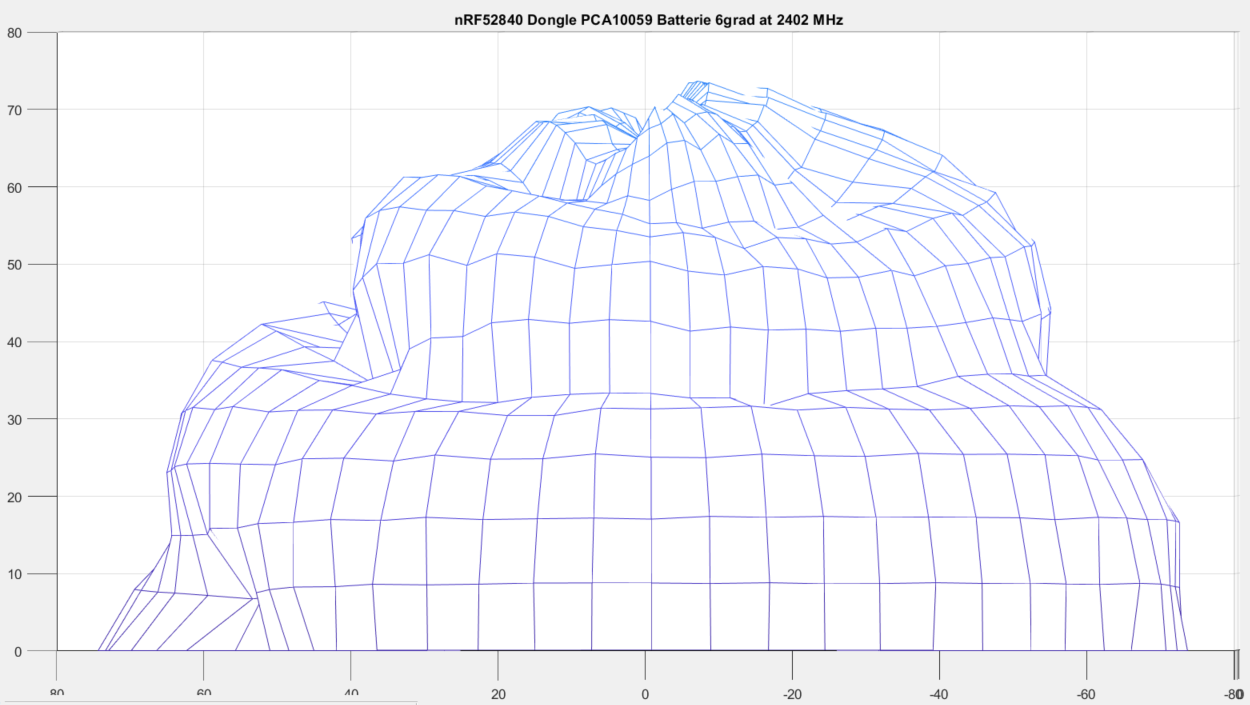
\includegraphics[width=\textwidth]{PCA10059_Peak.png}
	\caption{Abstrahlung in Z-Richtung PCA10059}
	\label{fig:PCA10059Peak}
\end{minipage}
\end{figure}

Die gemessenen Abstrahleigenschaften der beiden Antennen bestätigen schliesslich unsere Erfahrungen die wir mit den Boards bereits gemacht haben. Die MIFA Antenne des pca10059 weisst einige klare Nachteile gegenüber der IFA Antenne des pca10056 auf. Bei eingeschränkten Platzverhältnissen wie sie auf dem pca10059 und bei vielen Low-Power Mesh Anwendungen herrschen, ist jedoch eine MIFA eine solide Alternative.

Die Erkenntnisse aus den vorliegenden Messungen waren hilfreich bei der Planung und Durchführung der Mesh Benchmarks. Beim Aufbau der Testnodes \ref{subsec:AufbauTestnode} flossen diese beispielsweise ein um die Ausrichtung der Antenne zu optimieren. Weiter halfen die Ergebnisse bei der Interpretation der weiteren Messungen da auch dort klar aufgezeigt werden konnte, dass die Positionierung und Ausrichtung der Antenne von entscheidender Bedeutung für die Performance ist.

\subsection{Benchmark Management Station}\label{subsec:BenchmarkManagementStation}

Die Benchmark Management Station (BMS) ist im Mesh Benchmark und in der P2P Testinfrastruktur unterschiedlich ausgeführt. Im Mesh Benchmark handelt es sich um einen PC welcher via USB UART Verbindung mit dem Benchmark Master Node (BMN) verbunden ist. Dazu kann jeder PC verwendet werden.
Bei der P2P Testinfrastruktur stellt die BMS ein Raspberry Pi4 dar. Dieser wird ebenfalls wia USB UART mit dem BMN verbunden. Mit dem Einsatz eines Raspberry Pi's als BMS wird diese unabhängiger und kann einfach portiert werden. So kann die Testinfrastruktur als Messinstrument eingesetzt werden.


\pagebreak

\clearpage
\section{Soft- und Firmware}\label{sec:Soft-undFirmware}


Im folgenden Abschnitt werden Anforderungen, Konzept, Entscheidung und die Umsetzung der Software dokumentiert. Die Lösungsfindung und ihre Prozess wird nachfolgend beschrieben. 

\subsection{Anforderungen}\label{subsec:Software_Anforderungen}

Wie bereits im Abschnitt \ref{sec:Abgrenzung} wurden die Anforderungen in der Aufgabenstellung (siehe Anhang \ref{app:Aufgabenstellung}) sowie im Pflichtenheft (siehe Anhang \ref{app:Pflichtenheft}) vorgängig festgelegt. Im Fokus steht das erfassen der wichtigsten Messgrössen welche nachfolgend aufgeführt werden. \\

\begin{itemize}
	\item \textbf{Latenzzeit}: Bestimmung der Latenzzeit in Millisekunden zwischen den Teilnehmern. Die Genauigkeit sollte bei $+/-$1 ms liegen.  
	\item \textbf{Anzahl Hops}: Bestimmung der Anzahl Hops, über welche eine Nachricht übermittelt wird.
	\item \textbf{Datenrate}: Messen der Datenrate in Bytes/s, welche zwischen zwei Teilnehmern erreicht wurde. 
	\item \textbf{RSSI}: Erfassen des RSSI-Werts der eingehenden Pakete.
	\item \textbf{Paketverlust}: Pakete zählen, welche ihr Ziel nicht erreicht haben.  
	\item \textbf{Aktive Radio Zeit}: Erfassen der aktiven Radio-Zeit um den Energieverbrauch abschätzen zu können. 
\end{itemize}


Die Erfassung muss in allen Mesh-Netzwerken möglich sein. Um die Messresultate vergleichen zu können müssen die gleichen Ausgangslagen vorliegen, sowie die selben Messmethoden angewendet werden. 

\todo[inline]{Beschreiben der Anforderungen an die Software. Einzelne Teilprobleme Beschreiben}


\subsection{Konzept}\label{subsec:Software_Konzept}

Um die Messdaten erfassen zu können müssen alle Teilnehmer im Netzwerk eine eigenes Log führen. Dieses wird im Anschluss an eine zentrale Auswerte-Stelle übermittelt um ausgewertet zu werden (wie in Abschnitt ... beschrieben). Folgende Daten müssen pro eingehende oder gesendete Nachricht von allen Teilnehmern der Messung erfasst werden. 

\begin{itemize}
	\item \textbf{Message-ID}: Eindeutige Kennung (Laufnummer) welche beim Senden einer Nachricht mitgegeben wird. Somit können die Nachrichten anschliessend zugeordnet werden. 
	\item \textbf{Timestamp}: Erfassen der Sende- / Empfangszeit über synchronisierten Zeitwert. Relevant zur Bestimmung der Latenzzeit und Datenrate. 
	\item \textbf{Hops}: Auslesen der Anzahl Hops des Pakets beim Empfangen. Beim Senden kann dieser Wert ignoriert werden.
	\item \textbf{Source Address}: Erfassen der Teilnehmer-Addresse welcher die Nachricht sendet oder gesendet hat. Wichtig für die korrekte Zuordnung der Pakete. 
	\item \textbf{Destination Address}: Erfassen der Teilnehmer-Addresse welcher die Nachricht empfangen hat. Ebenfalls für Zuordnung der Nachrichten relevant. 
	\item \textbf{Group Address}: Erfassen der Gruppen-Adresse in welcher die Nachricht unterwegs war. Notwendig zur Erfassung des Paketverlustes. 
	\item \textbf{RSSI}: Erfassen des RSSI-Werts der eingehenden Pakete. Beim senden soll dieser Wert 0 sein. 
	\item \textbf{Paketgrösse}: Erfassen der Paketgrösse um die Datenrate zu berechnen. 
\end{itemize}

Zur Steuerung der Messungen wird eine zentrale Stelle (Master) verwendet (Wie in Abschnitt ... beschrieben). Diese soll einzelne Teilnehmer Konfigurieren, eine Messung starten, sowie die Reports  einsammeln können. 


\todo[inline]{Konzept zur Lösung der Teilprobleme grob beschreiben}


\subsection{Entscheidung}\label{subsec:Software_Entscheidung}

Zur Umsetzung der Mesh-Stacks mittles der \textit{NRF-Platform} sind folgende SDKs vorhanden: 

\begin{itemize}
	\item \textit{\textbf{nRF Connect SDK}}: Auf dem Zephyr-RTOS aufbauende SDK. Diese soll in Zukunft alle drei Mesh-Protokolle (Bluetooth-Mesh, Openthread und Zigbee) unterstützen. Wird jedoch noch nicht zum Einsatz in End-Produkten empfohlen. \cite{nordic_semi_welcome_to_the_nrf_connect_sdk_2020}
	\item \textit{\textbf{nRF SDK for Thread and Zigbee}}: Proprietäre SDK Library von Nordic Semiconductor. Thread integration mittels Openthread, Zigbee einbindung mittels ZBOSS. \cite{nordic_semi_nrf_sdk_for_thread_and_zigbee_2020}
	\item \textit{\textbf{nRF SDK for Mesh}}: Proprietäre SDK Library von Nordic Semiconductor für Bluetooth-Mesh. Ist zur Produktion freigegeben. \cite{nordic_semi_nrf_sdk_for_mesh_2020}
\end{itemize}

Die Messungen sollten trotz der verschiedenen Bibliotheken möglichst einheitlich sein, um die Vergleichbarkeit nicht zu beeinträchtigen. Daher musste ... Das Erfassen der Daten erfolgt Um eine möglichst unabhängig von der verwendeten Library zu sein wurde auf eine selbst entwickelte Kommunikation über die P2P-Testinfrastruktur gesetzt. 

\todo[inline]{Warum wurde die Software so umgesetzt?}

\todo[inline]{Tabelle der SDKs und Stacks und ihren Möglichkeiten aufzeigen. -> Gesamtheitliche Lösung mittels eigener Verwaltungsschicht und P2P}


\todo[inline]{Tabelle welche Software zu welchem Stack, Referenzen zu Parts}


\subsection{Umsetzung}\label{subsec:Software_Umsetzung}

\todo[inline]{Cyrill Tabelle und subsections, Raffel und Robin Text}



Die Software und Firmware für die Mesh Benchmarks sowie für die P2P Testinfrastruktur setzt sich aus diversen Modulen zusammen. Die Tabelle \ref{tab:UebersichtSoftware} zeigt eine Übersicht der wichtigsten Module und deren Verwendung in den 4 Benchmark Teilen: BLE Mesh, Zigbee, Thread sowie P2P.
Gemeinsame Module auf Firmware Ebene für die BT Mesh und Zigbee Firmware sind im Ordner SharedLib im Github Repository\footnotemark\ zusammengefasst. Aus diversen Gründen wurde die Thread Firmware zu einem grossen Teil in separaten Modulen realisiert. Die nicht Stack spezifischen Teile der Thread Lösung werden als Thread Common zusammengefasst.
Jene Python Scripts für das Benchmark Management stehen im gleichnamigen Ordner auf dem Github Repository zur Verfügung.
Die Stack bezogenen Implementationen der Benchmark Firmware werden in den individuellen Teilen \ref{part:BluetoothMesh}, \ref{part:Thread} und \ref{part:Zigbee} behandelt.


\newcommand{\rotcells}[1]{%
  \rotatebox[origin=c]{90}{ #1 }%
}
\begin{table}[h]
\centering
\begin{tabular}{|c|l|l|c|c|c|c|} 
\cline{4-7}
\multicolumn{1}{l}{} & \multicolumn{2}{l|}{} & \multicolumn{1}{l|}{BT Mesh} & Zigbee & Thread & P2P \\ 
\hline
\multirow{8}{*}{\rotcells{SharedLib}} & Statemachine & bm\_statemachine.c [\ref{subsubsec:Statemachine}]& x & x &  &  \\ 
\cline{2-7}
 & Timesync & bm\_timesync.c [\ref{subsubsec:Timesync}] & x & x &  & x \\ 
\cline{2-7}
 & Control & bm\_control.c [\ref{subsubsec:Control}] & x & x &  & x \\ 
\cline{2-7}
 & Report & bm\_report.c [\ref{subsubsec:Report}] & x & x &  & x \\ 
\cline{2-7}
 & Logging & bm\_log.c [\ref{subsubsec:Logging}]& x & x &  & x \\ 
\cline{2-7}
 & Flash Save & bm\_flash\_save.c [\ref{subsubsec:FlashSave}]& x & x &  &  \\ 
\cline{2-7}
 & CLI & bm\_cli.c [\ref{subsubsec:CLI}]& x & x &  & x \\ 
\cline{2-7}
 & Low Layer Radio & bm\_radio.c [\ref{subsubsec:LowLevelRadio}]& x & x &  &  \\ 
\hline
\multirow{4}{*}{\rotcells{\begin{tabular}[c]{@{}c@{}}Benchmark\\Management \end{tabular}}} & Flash & Flasher.py [\ref{subsubsec:Flash}]& x & x & x &  \\ 
\cline{2-7}
 & Configurator & Configurator.py [\ref{subsubsec:Configurator}]& x & x &  &  \\ 
\cline{2-7}
 & Benchmark & \begin{tabular}[c]{@{}l@{}}Benchmark\_and\_\\Reporter.py [\ref{subsubsec:Report}] \end{tabular} & x & x &  &  \\ 
\cline{2-7}
 & Analysis & Analysis.py [\ref{subsubsec:Analysis}]& x & x & x &  \\
\hline
\end{tabular}
\caption{Übersicht Shared Lib und Benchmark Management Module}
\label{tab:UebersichtSoftware}
\end{table}

Sämtliche Firm- und Software Komponenten die für Mesh Benchmark sowie die P2P Testinfrastruktur nötig sind, können auf dem Github Repository zum Projekt unter folgendem \href{https://github.com/Rouben94/P6_Software}{Link\footnotemark[\value{footnote}]}  eingesehen werden.

\footnotetext{\url{https://github.com/Rouben94/P6_Software} \cite{anklin_bobst_horath_rouben94p6_software_nodate}}




\subsection{Shared Library}\label{subsec:SharedLibrary}

Die \textit{Shared Library} ist die geteilte Bibliothek zwischen allen Mesh-Stacks. Sie beherbergt alle relevanten Module um eine Messung zu Verwalten. Der jeweilige Mesh-Stack ist lediglich für das senden und empfangen von Nachrichten, sowie zum Erfassen der Messdaten zuständig. 


\begin{figure}[H]
	\centering
	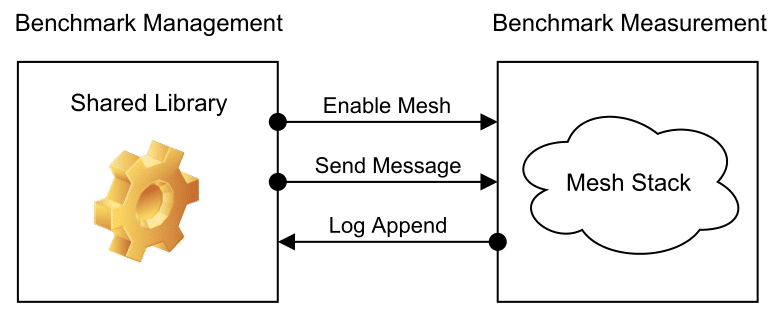
\includegraphics[width=0.6\textwidth]{Shared_Lib_Concept.png}
	\caption{Vereinfachte Anbindung der \textit{Shared Library} an die Mesh-Stacks}\label{fig:ShardeLibConcept}
\end{figure}

Abbildung \ref{fig:ShardeLibConcept} zeigt die vereinfachten Schnittstellen zwischen der Shared-Library und den Mesh-Stacks. Die Bibliothek ist spezifisch für die nRF52840 SOCs zugeschnitten. Um einfach in die jeweilige SDK integrierbar zu sein müssen die Module der Shared-Lib möglichst ohne weitere Abhängigkeiten klar kommen. Sofern Treiber oder externe Bibliotheken für Module benötigt werden, müssen diese von allen SDKs vergleichbar zur Verfügung gestellt werden. Im folgenden Abschnitt wird auf die einzelnen Module der \textit{Shared-Lib} eingegangen. 


\subsubsection{Statemachine}\label{subsubsec:StatemachineSoftware}

Die Statemachine dient dazu den Ablauf, welcher in Abschnitt \ref{subsec:AblaufMesh} beschrieben wurde abzuarbeiten. Sowohl der Master, die Server und Clients arbeiten den in Abbildung \ref{fig:StatemachineFLowgraph} dargestellten Ablauf ab. 

\begin{figure}[H]
	\centering
	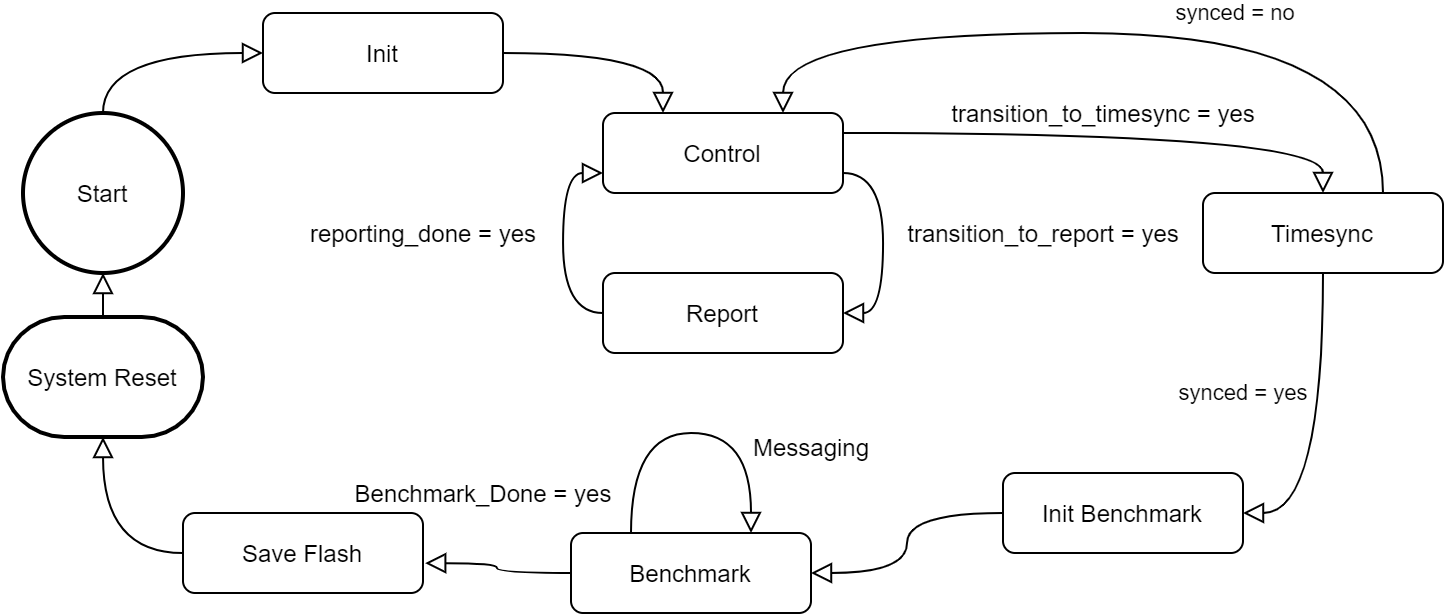
\includegraphics[width=1.0\textwidth]{Statemachine_Flowgraph.png}
	\caption{Flowgraph der Statemachine}\label{fig:StatemachineFLowgraph}
\end{figure}


Die Funktion der Schritte wird im Folgenden grob beschrieben. Zur genauen Untersuchung ist der Source Code unter \cite{rouben94_sharedlib_software_git_2020} verfügbar.  \\

\begin{itemize}
	\item \textbf{\textit{Init:}} Dieser Schritt initialisiert alle notwendige Funktionen (Radio, Timers, usw.). Ebenfalls rekonstruiert er die \textit{Log-Daten} indem er diese aus dem Flash in das RAM kopiert. Nach der erfolgreichen Initialisierung wechselt die Statemachine in den Control-State.
	\item \textbf{\textit{Control:}} Im Control-State wartet jeder Teilnehmer auf eingehende Befehle des Benutzers. Der Master erhält über das Command Line Interface (CLI) den auszuführenden Befehl. Diesen wandelt der Master in eine Nachricht (Control-Message) um und leitet sie über das Radio-Interface an die Slaves weiter.  Alle Slaves (Clients und Servers) erwarten eine Control-Message über das Radio-Interface. Damit alle Clients und Servers die Nachricht empfangen können wiederholt jeder Slave jede Control-Message. Somit wird die Mesh-Fähigkeit der Verwaltungsschicht (Benchmark Managment) sichergestellt. Folgende Transitionen sind vom Control-State zugelassen: 
	\begin{itemize}
		\item \textit{\textbf{Transition to Timesync}}: Wird ein Benchmark gestartet erfolgt dies durch einen Wechsel in den Timesync-State. Jeder Teilnehmer wechselt nach wiederholen der Nachricht in den entsprechenden Schritt. 
		\item \textit{\textbf{Transition to Report}}: Das Reporting wird über den Report-State abgehandelt. Nur der Teilnehmer von welchem Reports angefordert wurden, wechselt in den Report-State. 
	\end{itemize} 	
	\item \textbf{\textit{Timesync:}} Der Master verteilt die Zeitsynchronisation an die Slaves. Die Slaves synchronisieren sich auf das Signal des Masters auf, sofern sie in seiner Reichweite liegen. Sobald ein Slave synchronisiert ist, fängt er an die Zeitsynchronisation ebenfalls zu verteilen. Dadurch können Slaves, welche nicht über einen Hop vom Master erreicht werden sich ebenfalls synchronisieren. Konnte ein Slave keine Zeitsynchronisation durchführen, wechselt dieser in den  \textit{Control-State} zurück und bringt einen Fehler mittels der roten-LED zur Anezige. Der Master wird immer zum nächsten Schritt voranschreiten. 	
	\item \textbf{\textit{Init Benchmark:}} Dies ist der Zeitpunkt bei welchem jeder Teilnehmer den Mesh Stack-Initialisiert und Anschliessend Startet. Das Netzwerk hat nun Zeit sich aufzubauen, falls dies notwendig ist. Vor dem Initialisieren des Mesh-Stacks löscht jeder Node die Log-Daten aus dem Flash, sowie dem RAM. Beim Client wird zusätzlich der Sendezeitpunkt der Benchmark-Nachrichten (Benchmark-Messages) berechnet und vorbereitet. Hat sich der Slave erfolgreich Initialisiert und mit dem Netzwerk verbunden, beginnt das grüne Status-LED zu leuchten. Der wechsel zum Benchmark-State wird unabhängig vom Verbindungsstatus nach einer Verzögerungszeit ausgelöst. 
	\item \textbf{\textit{Benchmark:}} Die Statemachine wartet in diesem Schritt lediglich auf das auslösen von Events. Beim Server überlässt sie dem Mesh-Stack das Loggen der empfangenen Nachrichten, welcher über einen eigenen Event-Handler verfügt. Beim Client plant die Statemachine das senden von Nachrichten mittels Timer-Interrupts. Löst ein solcher aus, wird der Mesh-Stack sofort benachrichtigt. Das erfassen des Logs erfolgt ebenfalls im Stack. Der Status des einzelnen Slaves (Licht EIN / Aus) ist über die grüne RGB-LED (Client) oder die blaue RGB-LED (Server) erkennbar. Nach der eingestellten Benchmark-Zeit, löst der Letzte Timer-Interrupt aus und die Abarbeitung des Mesh-Stacks wird abgebrochen. Es folgt der wechsel zum letzten Schritt. 
	\item  \textbf{\textit{Save Flash:}} Das speichern der Log-Daten aus dem RAM in das Flash ist unabdingbar, damit diese persistent bleiben. Anschliessend wird der Mesh-Stack durch einen Reset des Mikrocontrollers heruntergefahren. Dies ist notwendig um sicherzustellen, das der Stack komplett deinitialisiert ist und das Radio-Interface für das Benchmark-Management zur verfügung steht. Zudem soll ein neuer Benchmark ohne Vorbelastung möglich sein. Nach dem Reset beginnt die Statemachine automatisch wieder von vorne im Init-State. 
	\item  \textbf{\textit{Reports:}} Das einholen von Reports ist nur über eine direkte Verbindung vom Master zum Slave möglich. Die Übertragung der Log-Einträge erfolgt über ein abgesichertes Handshake-Verfahren. Der Master sendet eine Anfrage und verlangt beim Slave den n-ten Log-Eintrag. Der Slave antwortet auf die Anfrage mit dem entsprechenden Log-Eintrag. Hat der Master diesen erhalten, so verlangt er den nächst höheren Eintrag. Andernfalls verlangt der Master den selben Eintrage erneut. Ist die Übetragung zu oft fehlgeschlagen wird das Reporting abgebrochen. Der Master und Slave wechseln beide nach erfolgreichem oder abgebrochenem Reporting in den Control-State zurück.  
\end{itemize}

\subsubsection{Timesync}\label{subsubsec:Timesync}



\subsubsection{Control}\label{subsubsec:Control}

\subsubsection{Report}\label{subsubsec:Report}

\subsubsection{Logging}\label{subsubsec:Logging}

\subsubsection{Flash Save}\label{subsubsec:FlashSave}

\subsubsection{CLI}\label{subsubsec:CLI}

\subsubsection{Low Level Radio}\label{subsubsec:LowLevelRadio}



\subsection{Thread Common}\label{subsec:ThreadCommon}

\subsubsection{Statemachine}\label{subsubsec:Statemachine}



\subsection{Benchmark Management}\label{subsec:Benchmark Management}

\subsubsection{Flash}\label{subsubsec:Flash}

\subsubsection{Configurator}\label{subsubsec:Configurator}

\subsubsection{Benchmark}\label{subsubsec:Benchmark}

\subsubsection{Analysis}\label{subsubsec:Analysis}


\pagebreak

%\clearpage
\section{Point to Point Testinfrastruktur}\label{sec:PointtoPointTestinfrastruktur}

\subsection{Messaufbau}\label{sec:Messaufbau}

\subsection{Ablauf}\label{sec:Ablauf}

\subsection{Aufbau und Bedienung der Messinfrastruktur}\label{sec:AufbauundBedienungderMessinfrastruktur}

\subsection{Interpretation der Messresultate für den Anwender}\label{sec:InterpretationderMessresultatefürdenAnwender}
%\pagebreak

%%Part 1 Bluetooth Mesh

\vspace*{4cm}
\part{Bluetooth Mesh}\label{part:BluetoothMesh}
Raffael Anklin
\vspace*{\fill}
\clearpage

\section{Einleitung}\label{sec:EinleitungBluetooth}


Bluetooth Mesh ist ein auf dem Bluetooth-Standard aufbauendes Mesh-Netzwerk. Der Standard wurde im Jahr 2017 von der Bluetooth-SIG vorgestellt. Das Ziel des Standards ist es die Reichweite und das Einsatzgebiet von Bluetooth-Geräten zu erweitern. Somit sollen in Zukunft Lichtschalter und Lampen, sowie Sensoren und Aktoren im Heimbereich, Industriebereich und diversen Anwendungsbereichen mittels Bluetooth-Technologie verbunden werden.  \\

\begin{figure}[!htbp]
	\begin{minipage}{0.49\textwidth}
		\centering
		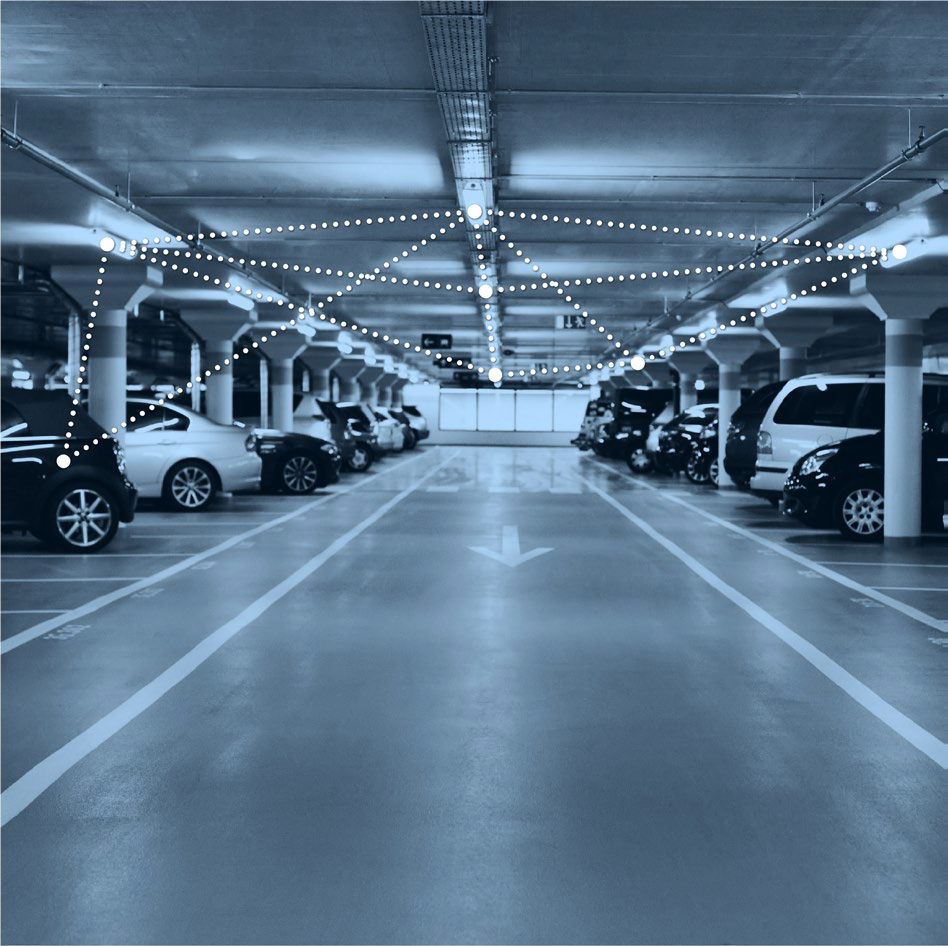
\includegraphics[width=\textwidth]{Bluetooth_Mesh_CarPark_Example.png}
		\caption[Parkhaus mit Bluetooth-Mesh]{Parkhaus mit Bluetooth-Mesh \cite{bluetooth_sig_mesh-technology-overviewpdf_2020}}
		\label{fig:BluetoothMeshParkingExample}
	\end{minipage}
	\begin{minipage}{0.49\textwidth}
		\centering
		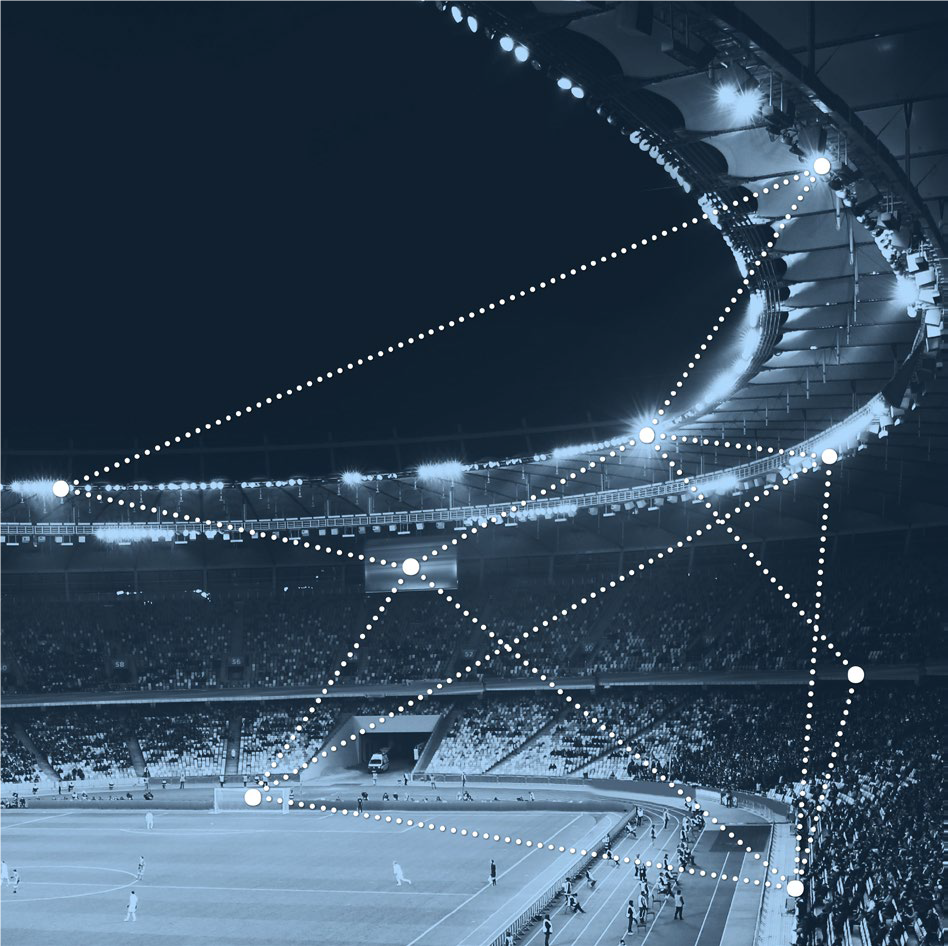
\includegraphics[width=\textwidth]{Bluetooth_Mesh_Stadium_Example.png}
		\caption[Stadion mit Bluetooth-Mesh]{Stadion mit Bluetooth-Mesh \cite{bluetooth_sig_mesh-technology-overviewpdf_2020}}
		\label{fig:BluetoothMeshStadiumExample}
	\end{minipage}
\end{figure}


Die Technologie baut auf den weit verbreitetem BLE-Standard auf, welcher in einer viel zahl von Endgeräten verbaut ist. Ab BLE-Version 4.0 könnten sich die Geräte zu einem Mesh-Netzwerk verbinden. Im Anschluss wird der Netzaufbau kurz erklärt und der Leser mit dem Funktionsprinzip des Mesh-Stacks vertraut gemacht.

Das Einbinden neuer Teilnehmer findet über den Provisioning-Prozess statt. Die Rolle des Provisioners kann ein Smartphone, Laptop oder ein berechtigter Mesh-Teilnehmer übernehmen. Ähnlich wie beim anmelden bei einem WLAN-Netzwerk teilt der Provisioner dem neuen Teilnehmer die Zugangsdaten (Netzwerkschlüssel, etc.) mit. Abschliessend beginnt das neue Gerät im Netzwerk als Node zu operieren. \\  


Bluetooth-Mesh basiert auf dem Managed-Flooding Prinzip. Einfach erklärt wiederholen alle Nodes, abhängig von verschiedenen Bedingungen, jede empfangende Nachricht (Relaying). Somit gelangen die Daten über Zwischenstationen (Hops) zum Ziel. Nachrichten welche nicht für den einzelnen Node relevant sind oder bereits verarbeitet wurden werden verworfen. \\

Um die Funktion von Nodes (Lichtschalter, Lampe, Temperatursensor, etc.) zu unterscheiden, werden sogenannte Models definiert. Jedes Model spezifiziert Zustände (Licht EIN / Licht AUS), welche als States bezeichnet werden. Weiterhin sind Models in drei Kategorien eingeteilt: Server-, Client- und Control-Models. Diese Einteilung schreibt vor ob die Zustände des Nodes zur Veränderung Angeboten werden (Server-Model z.B. Lampe), Zustände verändert werden (Client-Model z.B. Schalter) oder beides möglich ist (Control-Model z.B. Pumpe). Mithilfe dieser Normen lassen sich Geräte von unterschiedlichen Hersteller vereinen, sofern keine Hersteller spezifischen Models verwendet wurden. 

\begin{figure} [H]
	\centering
	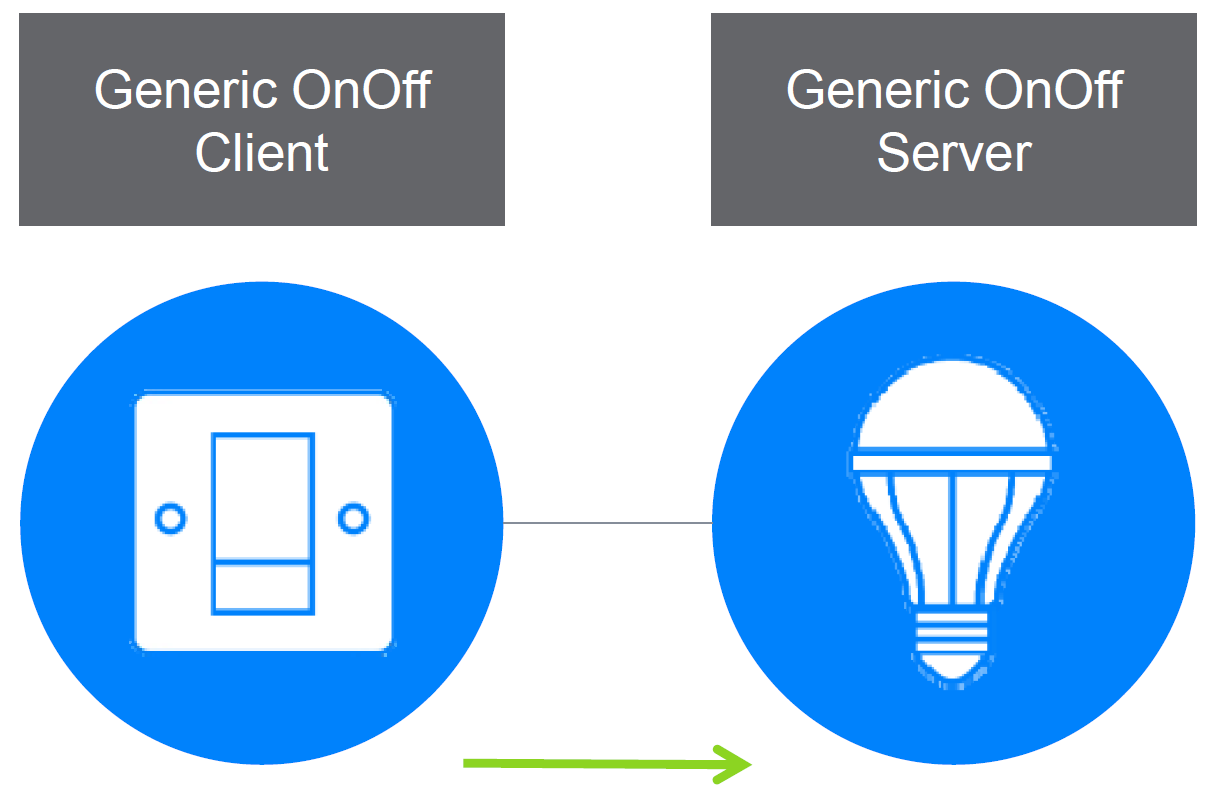
\includegraphics[width=0.6\textwidth]{Bluetooth_Mesh_Client_Server_Prinzip.PNG}
	\caption{Client - Server Prinzip Bluetooth Mesh \cite{bluetooth_sig_mesh-technology-overviewpdf_2020}} 
	\label{fig:BTMeshClientServerPrinzip}
\end{figure}


Zur Identifizierung im Netzwerk besitzt jeder Node eine Unicast-Address (einzigartige Adresse). Um mehrere Nodes zu einer Gruppe zusammenzufassen, werden Group-Addresses vergeben. Die Beziehungen zwischen Nodes werden durch Publishen (Veröffentlichen) oder Subscriben (Abonnieren) auf Adressen geregelt. Im Anwendungsfall Publisht der Client (Schalter) an die Adresse auf welche einer oder mehrere Server (Lampe/Lampen) Subscriben. Wie in Abbildung \ref{fig:BTMeshPublishSubscribePrinzip} ist das Unterscheiden von Bereichen mittels Gruppen möglich. Ein Node kann gleichzeitig an mehrere Adressen Publishen und Subscriben, was zu beliebig komplexen Aufbauten führt. 


\begin{figure} [H]
	\centering
	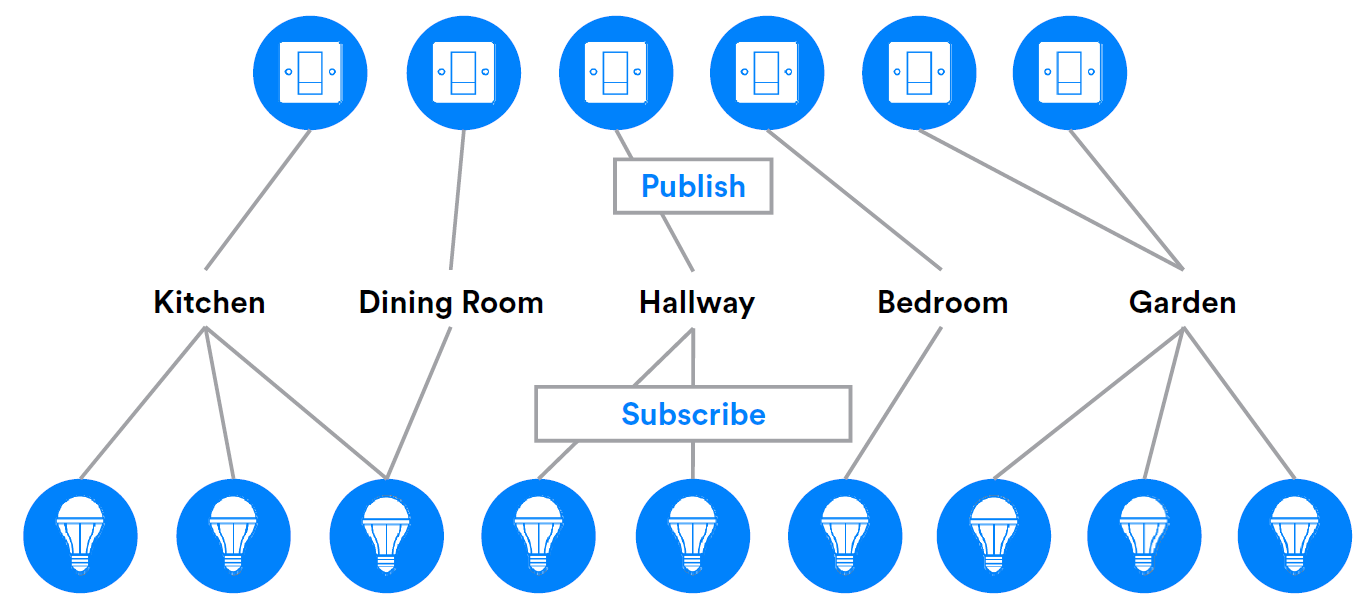
\includegraphics[width=1.0\textwidth]{Bluetooth_Mesh_Publish_Subscribe_Prinzip.PNG}
	\caption{Publish - Subscribe Prinzip Bluetooth Mesh \cite{bluetooth_sig_mesh-technology-overviewpdf_2020}} 
	\label{fig:BTMeshPublishSubscribePrinzip}
\end{figure}









\pagebreak

\clearpage
\section{Technische Grundlagen Bluetooth Mesh}\label{sec:TechnischeGrundlagenBluetoothMesh}

\subsection{Netzaufbau und Topologie}\label{sec:NetzaufbauundTopologie}




\todo[inline]{Welchen Aufbau? Welche Art von Mesh? Welche Nodetypen gibt es? Welche typischen Eigenschaften besitzt das Protokoll?}

\subsection{Bluetooth Mesh Protokoll Stack}\label{sec:ZigbeeProtokollStack}
\todo[inline]{Erläuterung des Protokoll Stacks. Möglichst viel Grafiken und nur so viel als nötig Prosa.}

\subsection{Bluetooth Mesh Software Development Kit}\label{sec:ZigbeeSoftwareDevelopmentKit}
\todo[inline]{Eingesetzte SDK und deren Aufbau beschreiben. Allenfalls die wichtigsten API Funktionen genauer erläutern.}



\pagebreak

\clearpage
\section{Umsetzung Benchmark}\label{sec:BTMeshUmsetzungBenchmark}

Die Umsetzung des Benchmarks, wurde gemäss den Anforderungen des Benchamrk-Konzepts (siehe Abschnitt \ref{sec:BenchmarkKonzeptMeshNetzwerke}) umgesetzt. Zudem wurden die Schnittstellen gemäss dem Software Konzept (siehe Abschnitt \ref{sec:Soft-undFirmware}) an die Shared-Library eingebaut. Im Anschluss wird auf die Umsetzung mittels der SDKs eingegangen, sowie die einzelnen Module dazu Beschrieben. 

\subsection{nRF Connect SDK}\label{subsec:BluetoothMeshUmsetzungnRFConnectSDK} 

Das aufsetzen der nRF Connect SDK, sowie das Installieren der IDE ist online\footnotemark\ Dokumentiert. Mithilfe von Beispielen\footnotemark\ und der Bluetooth-Mesh-API\footnotemark\ wurde die Umsetzung bewerkstelligt. Dabei gliedert sich das Programm in zwei Module welche Nachfolgend beschrieben werden.

\footnotetext{\url{https://developer.nordicsemi.com/nRF_Connect_SDK/doc/latest/nrf/getting_started.html}} 

\footnotetext{\url{https://developer.nordicsemi.com/nRF_Connect_SDK/doc/latest/nrf/samples.html}} 

\footnotetext{\url{https://developer.nordicsemi.com/nRF_Connect_SDK/doc/latest/zephyr/reference/bluetooth/mesh.html}} 

\subsubsection{Stack Initialisierung und Konfiguration}\label{subsubsec:BluetoothMeshUmsetzungnRFConnectSDKInitandConfig} 

Das Modul \textit{bm\_blemesh.c}\footnotemark\ dient zur Initialisierung des Stacks. Dazu wird die Funktion \linebreak\textit{bm\_blemesh\_enable()} aufgerufen. Diese führt die notwendigen Schritte aus um den Mesh-Stack hochzufahren. Nach erfolgreicher Initialisierung wird mit dem Provisioning weitergefahren. \\


\footnotetext{\url{https://github.com/Rouben94/P6_Software/blob/master/Bluetooth/Zephyr_Mesh/src/bm_blemesh.c}}


\paragraph{Self Provisioning}

Um ein vollautomatischen Testablauf zu gewährleisten, wurden die Sicherheitsschlüssel direkt im Code vorgegeben. Mittels der eigens dafür vorgesehenen API \textit{bt\_mesh\_provision} kann sich der Teilnehmer selbst ins Netzwerk einbinden. Dies ist nur zu Testzwecken empfohlen. Die Einbindung der Teilnehmer ins Netz erfolgt somit zuverlässig und unkompliziert.\\

\paragraph{Self Configuring}

Nach der erfolgreichen Einbindung ins Netz, beginnt der Node mit seiner Konfiguration. Ob es sich dabei um einen Client oder Server handelt muss zur Laufzeit bereits bekannt sein. Dies wurde zum Zeitpunkt der Kompilierung mittels der \textit{bm\_config.h} Datei festgelegt. Um Testnachrichten zu senden oder zu Empfangen wurde das Generic ON/OFF Server- resp. Client-Model eingesetzt. Des weiteren werden die Models initialisiert, an den Applikations-Key gebunden und die Publish- oder Subsrcibe-Adressen auf die jeweilige Group-Address konfiguriert. Diese Werte sind entweder aus der vorhergehenden Konfiguration bekannt oder wurden fest vorgegeben. Der Teilnehmer ist nun bereit Nachrichten zu Senden oder zu Empfangen. 


 
 

\subsubsection{Model Handler}\label{subsubsec:BluetoothMeshUmsetzungnRFConnectSDKModelHandler}

Das Modul \textit{bm\_blemesh\_model\_handler.c}\footnotemark\ beherbergt alle notwendigen Model-Handler, welche zum Senden oder Empfangen von Nachrichten aufgerufen werden. In den jeweiligen Handlern soll ein Log-Eintrag mit den entsprechenden Informationen aufgefüllt werden. 


\footnotetext{\url{https://github.com/Rouben94/P6_Software/blob/master/Bluetooth/Zephyr_Mesh/src/bm_blemesh_model_handler.c}}


\paragraph{Message Sending}

Um eine Nachricht zu senden wird eine universelle Schnittstelle der Shared-Library zur Verfügung gestellt. Diese kann mittels dem Aufrufen der Funktion \textit{bm\_send\_message(}) eine Nachricht versenden. Anschliessend wird der entsprechende Handler des Generic ON/OFF Clients benachrichtigt. Dieser wechselt den Zustand des grünen RGB-LEDs, speichert eine Log-Eintrag und schickt die Nachricht ab. Dieser wird, gemäss der Konfiguration des Nodes, acknowledged oder unacknowledged  und mit der zusätzlichen anzahl Bytes gesendet. 

\paragraph{Message Receiving} 

Sobald eine Nachricht vom Stack empfangen wurde, wird der Handler des Generic ON/OFF Servers benachrichtigt. Im Handler-Kontext sind viele notwendige Informationen für das Log bereits enthalten. Das erfassen des Zeitstempels und abfragen der Nachrichtenlänge wird über externe Funktionsaufrufe und Hilfsvariablen bewerkstelligt. Schlussendlich wird die blaue RGB-LED geschaltet, welches den erfolgreichen Empfang einer Nachricht anzeigt. 


\subsection{Benchmark und Stack Parameter}\label{subsec:BT_MESHBenchmarkundStackParameter}

Die Tabelle \ref{tab:BT_MESHBenchmarkundStackParameter} soll einen Überblick der verwendeten Paramter des Stacks geben. 



\begin{table}[h]
	\centering
	\begin{adjustbox}{width=1\textwidth}
		\begin{tabular}{|l|l|l|} 
			\hline
			Stack Init Time & 10000 ms & \begin{tabular}[c]{@{}l@{}}Zeit die benötigt wird um den Stack für den Benchmark\\zu initialisieren. \end{tabular} \\ 
			\hline
			\multicolumn{1}{l}{} & \multicolumn{1}{l}{} & \multicolumn{1}{l}{} \\ 
			\hline
			Node Type & Relay-Node & Alle Nodes werden als Relay-Nodes konfiguriert \\ 
			\hline
			Default~Group ID & 0xC000 & \begin{tabular}[c]{@{}l@{}}Zu diesem Wert wird der Index für die\textcolor[rgb]{0.502,0,0}{ }zugewiesene Gruppe\\addiert um damit die Gruppenzugehörigkeit festzulegen.\end{tabular} \\ 
			\hline
		\end{tabular}
	\end{adjustbox}
	\caption{Bluetooth Mesh Benchmark und Stack Parameter}
	\label{tab:BT_MESHBenchmarkundStackParameter}
\end{table}

Ein detailierte Konfiguration des Zephyr Kconfig kann übder den Source-Code\footnotemark\ abgefragt werden. 

\footnotetext{\url{https://github.com/Rouben94/P6_Software/blob/master/Bluetooth/Zephyr_Mesh/prj.conf}}


\subsection{nRF SDK for Mesh}\label{subsec:BluetoothMeshUmsetzungnRFSDKMesh} 

Die Umsetzung mittels der \textit{nRF SDK for Mesh} wurde noch nicht vollumfänglich abgeschlossen. Es liegen zurzeit Probleme beim Zugriff auf den Flash-Treiber vor, welche noch zu beheben sind. Die Umsetzung des Benchmarks wurde jedoch abgeschlossen und es können Nachrichten versandt sowie empfangen werden. Das Loggen der Informationen funktioniert ebenfalls. \\

Das aufsetzen der \textit{nRF SDK for Mesh}, sowie das Installieren der IDE ist online\footnotemark\ Dokumentiert. Mithilfe von Beispielen\footnotemark\ und der Bluetooth-Mesh-API\footnotemark\ wurde die Umsetzung bewerkstelligt. Dabei gliedert sich das Programm in zwei Module, welche Nachfolgend beschrieben werden.\\

Die Umsetzung wurde ähnlich realisiert wie mit der \textit{nRF Connect SDK}. Im Anschluss sind die Unterschiede aufgezeigt. 



\footnotetext{\url{https://infocenter.nordicsemi.com/topic/com.nordic.infocenter.meshsdk.v4.2.0/md_doc_getting_started_getting_started.html}} 

\footnotetext{\url{https://infocenter.nordicsemi.com/topic/com.nordic.infocenter.meshsdk.v4.2.0/md_examples_light_switch_README.html}} 

\footnotetext{\url{https://infocenter.nordicsemi.com/topic/com.nordic.infocenter.meshsdk.v4.2.0/modules.html}} 

\subsubsection{Stack Initialisierung und Konfiguration}\label{subsubsec:BluetoothMeshUmsetzungnRFSDKInitandConfig} 

Das Modul \textit{bm\_ble\_mesh.c}\footnotemark\ sowie das Modul \textit{bm\_mesh\_stack.c}\footnotemark\ dienen zur Initialisierung des Stacks. Dazu wird die Funktion \textit{bm\_blemesh\_init()} aufgerufen. Diese führt die notwendigen Schritte aus um den Mesh-Stack hochzufahren. Nach erfolgreicher Initialisierung wird mit dem Provisioning weitergefahren. \\


\footnotetext{\url{https://github.com/Rouben94/P6_Software/blob/master/Bluetooth/nRF_SDK_Mesh/src/bm_ble_mesh.c}}

\footnotetext{\url{https://github.com/Rouben94/P6_Software/blob/master/Bluetooth/nRF_SDK_Mesh/src/bm_mesh_stack.c}}

\paragraph{Self Provisioning and Configuring}

Das Self Provisioning sowie das Self Configuring werden bei der \textit{nRF SDK for Mesh} mittels dem Device-State-Manager durchgeführt. Dieser verwaltet alle notwendigen Keys sowie Address-Listen, welche zur Konfiguration gebraucht werden. Durch analysieren des Config-Server-Models, welches normalerweise die Konfiguration des Nodes vornimmt, wurde der notwendige Ablauf zur Konfiguration rekonstruiert. 

\subsubsection{Model Handler}\label{subsubsec:BluetoothMeshUmsetzungnRFSDKModelHandler}

Die Model-Handler sind im Modul \textit{bm\_ble\_mesh.c}\footnotemark\ integriert. Das Empfangen und Senden von Nachrichten wird ähnlich wie bei der \textit{nRF Connect SDK} abgehandelt. 

\pagebreak

\clearpage
\section{Analyse Bluetooth Mesh Stack}\label{sec:AnalyseBluetoothMeshStack}

Bleutooth-Mesh ist ein relativ neuer Stack mit wenig Anwendungsbeispielen. Er wurde designed um mit der Konkurenzwie Z-Wave oder Zigbee mithalten zu können. Im folgenden werden die Grenzen des Stacks aufgezeigt, sowie die Praktische Erfahrung erläutert.



\subsubsection{Grenzen des Stacks}\label{subsec:BLEMeshProtokollStack}

Die Topologie eines Netzwerks beeinträchtigt stark seine Performance. Ist die Node-Dichte sehr hoch, steigt die Wahrscheinlichkeit an das es zu Kollisionen der einzelnen Nachrichten kommt. Der BLE-MAC-Layer verfügt im Gegensatz zum IEEE 802.15.4 Layer über keine Collision Avoidance. Somit ist es im Interesse aller Teilnehmer wenn die Radio-Sende-Zeiten so kurz wie möglich gehalten werden. Deshalb schreibt der Stack lediglich 29Bytes als maximale Network-PDU vor. Durch die Geschwindigkeit des MAC-Layers von 1-2Mbit/s sinkt die Wahrscheinlichkeit von Kollisionen der Pakete weiter. Das versenden von längeren Nachrichten, welche stark Segmentiert werden müssen, erhöhen die Gesamtbelastung des Netzwerks und sind somit eher unerwünscht. \cite{bluetooth_sig_mesh_netzwerk_spezifikationen_2020}\\

Der Mesh-Stack schreibt eine maximale Grösse von 32767 Teilnehmern vor. Dies soll die theoretische sowie praktische Grenze darstellen. Eine Gebäude der Firma Silvair wurde mit über 1000 Bluetooth-Mesh-Nodes ausgestattet. Laut dem Betreiber laufe das System einwandfrei. Dabei handelt es sich um ein Office-Gebäude mit vielen anderen Bluetooth-Geräten wie Smartphones, Mäuse und Headsets sowie WLAN-Access-Points.  \cite{woolley_how_bluetooth_mesh_puts_the_large__2018}

Ein Bluetooth-Mesh Paket wird immer auf drei Kanälen (37,38,39) gesendet (BLE-GAT Advertising). Dadurch erhöht sich die Störfestigkeit. Jedoch verringert sich der Durchsatz mit dem Faktor drei, da ein Paket dreimal solange braucht um gesendet zu werden. 

\subsubsection{Bluetooth Mesh Implementation in Zephyr}\label{subsec:BLEMeshProtokollStackZephyr}

Die Implementation des Bluetooth-Mesh-Stacks in Zephyr zeigte einige Unschönheiten. Es liegen Probleme mit dem HCI-Treiber (Host Controller Interface), welcher das Radio-Interface ansteuert, vor. Diese äussern sich dadurch, dass nach jedem Advertising (Senden) eines Mesh-Pakets  der aktive Thread für 10ms pausiert wird. Dadurch erhält die Abarbeitung des Stacks eine gravierende Verzögerung, bis wieder in den Scanner (Empfangs) Betrieb gewechselt werden kann. Vermutlich führt diese Lücke ebenfalls zum verkürzen der Aktive-Radio-Time, welche gemessen wird um den Energieverbrauch abzuschätzen. Sie gibt an wie lange das Radio-Interface aktiv genutzt wurde. 

Zudem wurde einen Problematik beim Segmentieren von Nachrichten in der Bluetooth-Mesh Implementation in Zephyr festgestellt. Beim Empfangen von segmentierten Nachrichten, werden diese zum Teil mehrmals empfangen. Ob dies Ebenfalls einen Einfluss auf das Messresultat hatte ist unklar. Ein Online\footnotemark\ Beitrag verweist ebenfalls auf diese Problematik. 

\footnotetext{\url{https://github.com/zephyrproject-rtos/zephyr/issues/16886}}



\pagebreak


%%Part 2 Thread

\vspace*{4cm}
\part{Thread}\label{part:Thread}
Robin Bobst
\vspace*{\fill}
\clearpage

\section{Einleitung}\label{sec:EinleitungThread}
Thread ist ein auf IPv6 basiertes Netzwerkprotokoll, das speziell für Internet of Things (IoT) Anwendungen entwickelt wurde. Die einzelnen Teilnehmer im Netzwerk verbinden sich zu einem Mesh-Netzwerk. Wie in der Abbildung \ref{fig:ThreadProtokollLayer} ersichtlich verwendet Thread für eine effiziente Kommunikation mit IPv6-Paketen das Kommunikationsprotokoll 6LoWPAN (IPv6 over Low Power Personal Area Network). 6LoWPAN wendet ein Header-Kompressionsverfahren an, welches es ermöglicht die IPv6-Pakete über den Standard IEEE-802.15.4 zu übermitteln. Dank diesem Standard ist es machbar, die mit Thread entwickelten Geräte so energieeffizient zu gestalten, dass ein Batteriebetrieb realisierbar ist. In der Tabelle \ref{table:MerkmaleThread} sind die wichtigsten Merkmale von Thread aufgelistet. Im Juli 2014 wurde die Thread Working Group ins Leben gerufen, bei der folgende Firmen Bestandteil der Gruppe sind: Nest Labs, Samsung, ARRM Holdings, Qualcom, NXP Semiconductors, Silicon Labs, Big Ass Solutions, Somfy, OSRAM Tyco International und Yale. Ab August 2018 Apple trat auch Apple der Arbeitsgruppe bei, um das Prokoll populär zu machen. \cite[Kapitel 1]{thread_group_inc_thread_2017} \\

\begin{figure}[H]
	\centering
	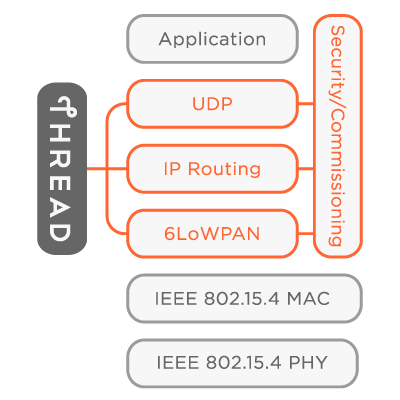
\includegraphics[width=0.5\textwidth]{threadlayerprotocols.png}
	\caption{Thread Protokoll Layer \cite{erickson_picture_2019}}
	\label{fig:ThreadProtokollLayer}
\end{figure}

\begin{table}[H]
	\centering
	\begin{adjustbox}{width=1\textwidth}
	\begin{tabular}{@{}lllll@{}}
		\cmidrule(r){1-2} \cmidrule(l){4-5}
		\multicolumn{2}{|c|}{\textbf{Netzwerk}}                                                              & \multicolumn{1}{l|}{} & \multicolumn{2}{c|}{\textbf{Applikation}}                                                                           \\ \cmidrule(r){1-2} \cmidrule(l){4-5} 
		\multicolumn{1}{|l|}{\textbf{Merkmal}}      & \multicolumn{1}{l|}{\textbf{Beschreibung}}             & \multicolumn{1}{l|}{} & \multicolumn{1}{l|}{\textbf{Merkmal}}                   & \multicolumn{1}{l|}{\textbf{Beschreibung}}                \\ \cmidrule(r){1-2} \cmidrule(l){4-5} 
		\multicolumn{1}{|l|}{IEEE 802.15.4}         & \multicolumn{1}{l|}{Protokoll}                         & \multicolumn{1}{l|}{} & \multicolumn{1}{l|}{IPv6}                               & \multicolumn{1}{l|}{IP-Kommunikation}                     \\ \cmidrule(r){1-2} \cmidrule(l){4-5} 
		\multicolumn{1}{|l|}{MAC Security}          & \multicolumn{1}{l|}{Verschlüsselte Übertragung}        & \multicolumn{1}{l|}{} & \multicolumn{1}{l|}{UDP}                                & \multicolumn{1}{l|}{UDP-Sockets}                          \\ \cmidrule(r){1-2} \cmidrule(l){4-5} 
		\multicolumn{1}{|l|}{6LoWPAN}               & \multicolumn{1}{l|}{Effiziente IPv6 Paket Übertragung} & \multicolumn{1}{l|}{} & \multicolumn{1}{l|}{CoAP}                               & \multicolumn{1}{l|}{Client und Server}                    \\ \cmidrule(r){1-2} \cmidrule(l){4-5} 
		\multicolumn{1}{|l|}{Mesh Routing}          & \multicolumn{1}{l|}{Many-to-many Kommunikation}        & \multicolumn{1}{l|}{} & \multicolumn{1}{l|}{DHCPv6}                             & \multicolumn{1}{l|}{Client und Server}                    \\ \cmidrule(r){1-2} \cmidrule(l){4-5} 
		&                                                        &                       &                                                         &                                                           \\ \cmidrule(r){1-2} \cmidrule(l){4-5} 
		\multicolumn{2}{|c|}{\textbf{Boarder Router}}                                                        & \multicolumn{1}{l|}{} & \multicolumn{2}{c|}{\textbf{Weitere Merkmale}}                                                                      \\ \cmidrule(r){1-2} \cmidrule(l){4-5} 
		\multicolumn{1}{|l|}{Web - UI}              & \multicolumn{1}{l|}{Für Netzwerk Menagement}           & \multicolumn{1}{l|}{} & \multicolumn{1}{l|}{Periodic parent search}             & \multicolumn{1}{l|}{Endgerät wechselt zu besserem Parent} \\ \cmidrule(r){1-2} \cmidrule(l){4-5} 
		\multicolumn{1}{|l|}{Externer Kommissioner} & \multicolumn{1}{l|}{Externes Gerät für Neuaufnahme}    & \multicolumn{1}{l|}{} & \multicolumn{1}{l|}{Jam Detection}                      & \multicolumn{1}{l|}{Signal Stau verhindern}               \\ \cmidrule(r){1-2} \cmidrule(l){4-5} 
		\multicolumn{1}{|l|}{NAT64}                 & \multicolumn{1}{l|}{Kommunikation mit IPv4}            & \multicolumn{1}{l|}{} & \multicolumn{1}{l|}{Child Supervision}                  & \multicolumn{1}{l|}{Endgerät überprüfen}                  \\ \cmidrule(r){1-2} \cmidrule(l){4-5} 
		\multicolumn{1}{|l|}{wpantund}              & \multicolumn{1}{l|}{Interface Treiber}                 & \multicolumn{1}{l|}{} & \multicolumn{1}{l|}{Inform previous parent on reattach} & \multicolumn{1}{l|}{Endgerät Menagement}                  \\ \cmidrule(r){1-2} \cmidrule(l){4-5} 
	\end{tabular}
	\end{adjustbox}
	\caption{Merkmale Thread \cite{thread_group_what_2020}}
	\label{table:MerkmaleThread}
\end{table}


\pagebreak

\clearpage
\section{Technische Grundlagen Thread}\label{sec:TechnischeGrundlagenThread}

\subsection{Netzaufbau und Topologie}\label{subsec:NetzaufbauundTopologie}
\todo[inline]{Welchen Aufbau? Welche Art von Mesh? Welche Nodetypen gibt es? Welche typischen Eigenschaften besitzt das Protokoll?}
\subsubsection{Node Typen}\label{subsubsec:NodeTypen}
\textbf{Full Thread Device (FTD)}

\underline{Leader:}

\underline{Router:}

\underline{Full End Device:}

\textbf{Minimal Thread Device (MTD)}

\underline{Minimal End Device:}

\underline{Sleepy End Device:}

\subsubsection{IPv6 Adressierung}\label{subsubsec:IPv6Adressierung}

\subsubsection{Netzwerk Aufbau}\label{subsubsec:NetzwerkAufbau}

\subsubsection{Router Auswahl}\label{subsubsec:RouterAuswahl}

\subsection{Application Layer}\label{subsec:CoAP}

\subsection{Thread Protokoll Stack}\label{subsec:ThreadProtokollStack}
\todo[inline]{Erläuterung des Protokoll Stacks. Möglichst viel Grafiken und nur so viel als nötig Prosa.}
\subsubsection{UDP}\label{subsubsec:UDP}
\subsubsection{IP Routing}\label{subsubsec:IPRouting}
\subsubsection{6LoWPAN}\label{subsubsec:6LoWPAN}

\subsection{Link und Physical Layer}\label{subsec:IEE802154}

\subsection{Thread Software Development Kit}\label{subsec:ThreadSoftwareDevelopmentKit}
\todo[inline]{Eingesetzte SDK und deren Aufbau beschreiben. Allenfalls die wichtigsten API Funktionen genauer erläutern.}

\pagebreak

\clearpage
\section{Firmware Benchmark}\label{sec:FirmwareBenchmark}
\todo[inline]{Komplette Beschreibung der Firmware unterteilt in die 3 Nodetypen. Besonderheiten herausstreichen und allfällige Schwierigkeiten aufzeigen.}


\subsection{Benchmark Master}\label{sec:BenchmarkMasterThread}


\subsection{Benchmark Server}\label{sec:BenchmarkServerThread}


\subsection{Benchmark Client}\label{sec:BenchmarkClientThread}
\pagebreak

\clearpage
\section{Analyse Thread Stack}\label{sec:AnalyseThreadStack}
In diesem Kapitel wird die persönliche Erfahrung mit dem Mesh-Stack zu Tage gelegt, die während des ganzen Entwicklungsprozesses entstanden ist.

\subsection{Vor- und Nachteile Openthread Stack}\label{susec:ThreadVorNachteile}
Nachfolgend werden die wichtigsten Vor- und Nachteile beschrieben, die sich als persönliche Erfahrung beschreiben lässt.
\paragraph{Vorteile}
Der Openthread Stack von Google Nest ist auf der Webseite \href{https://openthread.io/}{Openthread\footnote{\url{https://openthread.io/}}} sehr gut beschrieben. Es gibt eine kurze Einleitung wie der Stack funktioniert, ohne dabei zu grob ins Detail zu gehen. Weiter sind phantastische Tutorials auf der Webseite verfügbar, mit denen man beginnt ein Thread Netzwerk zu simulieren. Danach wird man Schritt für Schritt angeleitet mit einem SoC ein reales Netzwerk aufzubauen. Zum Schluss, wenn man das minimale Netzwerk erfolgreich aufgebaut hat, wird man auf die API verwiesen. Diese ist auch sehr Dokumentiert und man kann alle Funktionen die benötigt werden einfach suchen.

\paragraph{Nachteile}
Ein grosser Nachteil des Projekts von Google Nest ist die Beschreibung der API. Die Dokumentation ist lückenlos, jedoch wäre es sehr praktisch einige Beispiele der wichtigsten Funktionen zu haben. Meistens ist es schwierig die API Funktionen zu implementieren, da mehrere Parameter eingestellt werden müssen und dies in einem kurzen Beispiel gut ersichtlich wäre. Ein weiterer Nachteil ist das auslesen der Message ID. Dies ist nicht immer zuverlässig möglich. Dadurch musste mit der Payload der Benchmark Message eine Message ID mitgegeben werden. Aus diesem Grund wurde die Messung mit Acknowledgement nicht umgesetzt, da die Message ID nicht mit der Acknowledge Nachricht mitgegeben werden konnte. Das resultiert, dass die Nachrichten nicht identifiziert werden können.

\subsection{FreeRTOS Projekt}\label{susec:FreeRTOS Projek}
Auf dem \href{https://github.com/Rouben94/P6_Software}{Github-Repository\footnote{\url{https://github.com/Rouben94/P6_Software}\cite{anklin_bobst_horath_rouben94p6_software_nodate}}} ist ein Branch namens openthread\_freerots verfügbar. Das Openthread Projekt wurde zuerst auf Basis von FreeROTS entwickelt und ist grundsätzlich voll funktionsfähig. Es gab ein grosses Problem, das bis zum Schluss nicht behoben werden konnte. Aus diesem Grund wurde das Projekt in die Shared Lib \ref{subsec:SharedLibrary} implementiert. Das Problem war, dass sich ab ca. 10 Knoten Netzwerkgrösse, der SoC nRF52840 nach einiger Zeit in einen Hardfault verfing. Das Problem trat sporadisch und sehr zufällig auf. Es wird vermutet, dass sich das auf die RAM Benutzung des SoCs zurückzuführen lässt. Laut Google Nest vergrössert sich das RAM mit steigender Anzahl Knoten im Netzwerk. Da das RAM schon zu 50\% mit dem Projekt belegt wäre es möglich, dass dies der Grund ist des sporadisch auftretenden Hardfault des SoCs.
\pagebreak


%%Part 3 Zigbee

\vspace*{4cm}
\part{Zigbee}\label{part:Zigbee}
Autor: Cyrill Horath
\vspace*{\fill}
\clearpage

\section{Einleitung}\label{sec:EinleitungZigbee}
In diesem Teil der Arbeit werden die Eigenschaften und Besonderheiten des Zigbee Mesh Stack erläutert und es wird auf die Umsetzung des Benchmarks auf Stack Ebene eingegangen. Dieser Teil soll als eigenständiger Teil betrachtet werden in dem ausschliesslich Zigbee behandelt wird.

Zigbee ist ein auf dem IEEE 802.15.4 Standard aufbauendes drahtloses Low Power Mesh Netzwerk. Es nutzt das vom IEEE 802.15.4 Standard definierte ISM-Funkfrequenzband 2.4GHz plus weitere Sub-GHz Bänder je nach Region.
Die im Jahre 2002 gegründete Zigbee Allianz spezifiziert den Protokoll Standard und gibt seit da an laufend Neuerungen und Updates heraus.
Im Zuge der Verbreitung von Technologien in der Heim Automatisierung erhielt auch Zigbee immer mehr Aufmerksamkeit und wuchs bis heute zum wohl am weitesten verbreiteten Mesh Netzwerk Protokoll in diesen Gebiet heran. Besonders in Systemen für die Steuerung von Beleuchtungen wie zum Beispiel Phillips Hue und Ikea Tradfri kommt Zigbee verbreitet zum Einsatz.

Die Spezifikationen innerhalb des Zigbee Protokollstacks sind weitreichend. Von der MAC Ebene über die Netzwerkschicht bis hin zur Applikationsebene gibt es klare Vorgaben wie ein Zigbee Produkt aufgebaut sein soll.
Mit der \textit{Zigbee Cluster Library} werden sogar spezifische Anwendungen vordefiniert wie beispielsweise die Steuerung eine Lichtquelle mit Dimmfunktion.
Diese Spezifikationen ermöglichen die Interoperabilität von Systemen mit der gleichen Funktion jedoch von unterschiedlichen Herstellern.





\pagebreak

\clearpage
\section{Technische Grundlagen Zigbee}\label{sec:TechnischeGrundlagenZigbee}

\subsection{Netzaufbau und Topologie}\label{subsec:NetzaufbauundTopologie}
\todo[inline]{Welchen Aufbau? Welche Art von Mesh? Welche Nodetypen gibt es? Welche typischen Eigenschaften besitzt das Protokoll?}


Zigbee ist nicht gleich Zigbee. Obwohl Zigbee von zentraler Stelle, der Zigbee Alliance, spezifiziert wurde gibt es verschiedene Arten davon. In den Spezifikationen wird zwischen zwei sogenannten Stackprofilen \textit{ZigBee} und \textit{ZigBee PRO} unterschieden.
Während \textit{ZigBee}-Netzwerke eine Baumstruktur haben und der Koordinator dabei einen Single-Point-of-Failure bildet, bieten \textit{ZigBee PRO}-Netzwerke geroutete Mesh Funktionalitäten mit Routing Tabellen und Wegentdeckung. Der Koordinator bildet dabei nicht länger einen Single-Point-of-Failure da sich das Routing dynamisch anpassen kann.
Die Abbildung \ref{fig:NetzwerktopologienZigbee} zeigt die Unterschiede von einem Baumnetzwerk im Stackprofil \textit{ZigBee} links und einem Meshnetzwerk im Stackprofil \textit{ZigBee PRO} rechts.
In der vorliegenden Arbeit wurde das \textit{ZigBee PRO} Stackprofil verwendet womit vollwertige Meshnetzwerke möglich sind.

\begin{figure}[h]
	\centering
	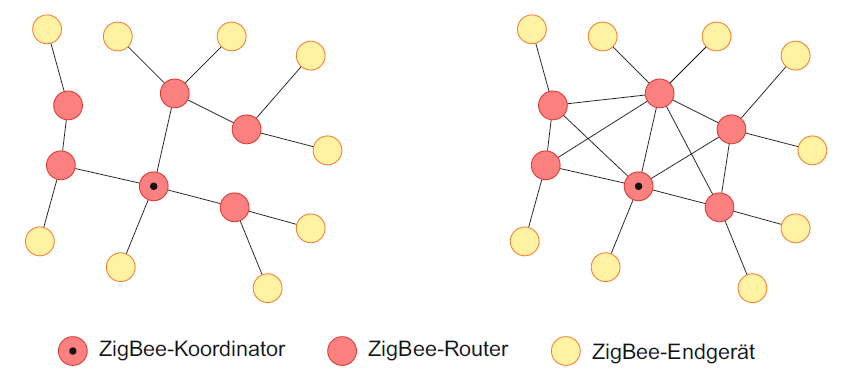
\includegraphics[width=0.8\textwidth]{Zigbee_Netztopologie.png}
	\caption{Zigbee Baum- und Meshnetzwerke \cite[S.~221]{markus_krause_rainer_konrad_zigbee_2014}}	\label{fig:NetzwerktopologienZigbee}
\end{figure}

Wie in der Abbildung \ref{fig:NetzwerktopologienZigbee} bereits angedeutet, kann innerhalb eines Zigbee Meshnetzwerkes zwischen 3 Nodetypen unterschieden werden. Diese besitzen unterschiedliche Aufgaben und Eigenschaften.

\paragraph{Zigbee Koordinator}\label{par:ZigbeeKoordinator}
Als zentrale Einheit übernimmt der \textit{Zigbee Koordinator} Aufgaben wie den Start und die Verwaltung eines PAN (Personal Area Network) inkl. der Definition der wichtigsten Parameter wie der PAN-ID, der Sicherheitsschlüssel sowie die Wahl des IEEE Channels.
In einem Zigbee-Netzwerk gibt es genau ein Gerät das die Rolle des \textit{Zigbee Koordinators} übernimmt. Wenn dieses Gerät das Netzwerk verlässt oder kurzzeitig ausser Betrieb ist, kann das Netzwerk trotzdem weiter bestehen und funktioniert normal weiter.
Jeder \textit{Zigbee-Koordinator} hat gleichzeitig auch die Rolle eines \textit{Zigbee-Router}.

\paragraph{Zigbee Router}\label{par:ZigbeeRouter}
\textit{Zigbee-Router} bilden das eigentliche Meshnetzwerk. Sie übernehmen die Aufgabe des Routings was die Wegentdeckung sowie Weiterleitung von Paketen beinhaltet. Jeder \textit{Zigbee-Router} führt eine Routing-Table welche fortlaufend aktualisiert wird.

\paragraph{Zigbee End-Device}\label{par:ZigbeeEndDevice}
Die einfachste Rolle ist jene des \textit{Zigbee End-Devices}. Sie stehen in einer Parent-Child Beziehung mit einem \textit{Zigbee-Router}.
Diese Kommunikation findet entweder periodisch oder ausgelöst durch einen Userinput statt.
Ankommende Pakete werden jeweils vom Parent-Node gespeichert bis das  \textit{Zigbee End-Devices} diese abruft.
\textit{Zigbee End-Devices} besitzen ausserdem keine Routing Funktionen und gelten deshalb als sehr energiesparend.
Ausgeführt als Sleepy-End-Device können CPU und RAM des entsprechenden Nodes ganz oder teilweise heruntergefahren werden und durch periodische Interrupts geweckt werden.
Dadurch können sehr lange Batteriestandzeiten erreicht werden. \cite{markus_krause_rainer_konrad_zigbee_2014}


\subsection{Zigbee Protokoll Stack}\label{subsec:ZigbeeProtokollStack}
\todo[inline]{Erläuterung des Protokoll Stacks. Möglichst viel Grafiken und nur so viel als nötig Prosa.}

Die Architektur des Zigbee Stacks besteht aus vier Layern, dem Physical layer (PHY), dem MAC layer, dem Network layer (NWK) und dem Application layer (APL).
Abbildung \ref{fig:ArchitekturdesZigbeeProtokollStacks} zeigt den Aufbau des Protokoll Stacks im Detail.
Jede der Schichten ist mit bestimmten Aufgaben betraut und stellt der darüber liegenden Schicht Daten und Dienste bereit.
Nachfolgend wird auf die vier Schichten des Zigbee Stacks eingegangen und deren Funktion und Funktionsweise kurz erläutert.

\begin{figure}[h]
	\centering
	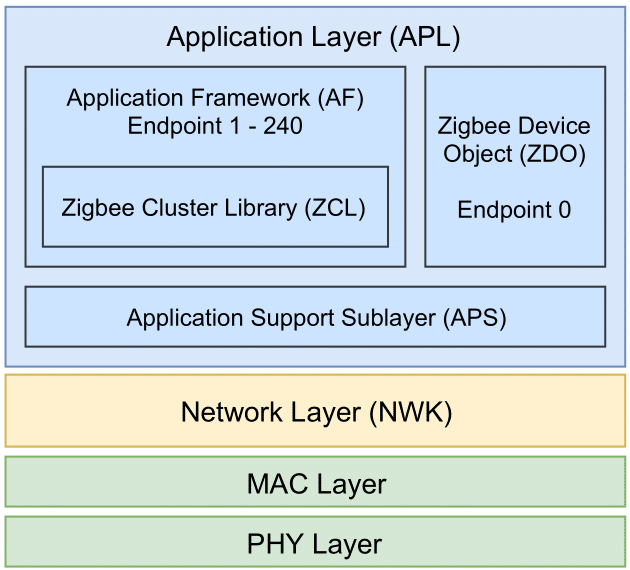
\includegraphics[width=0.7\textwidth]{Zigbee_Architektur.png}
	\caption{Architektur des Zigbee Protokoll Stacks}
	\label{fig:ArchitekturdesZigbeeProtokollStacks}
\end{figure}

\subsubsection{MAC und PHY Layer}\label{subsubsec:MACundPHYLayer}
MAC und PHY Layer werden im Zigbee Protokoll Stack gebildet durch den IEEE 802.15.4 Standard für \textit{Wireless Personal Area Networks (WPAN)}.
Während beispielsweise Wifi oder Bluetooth, welche auf dem selben 2.4 GHz ISM-Funkfrequenzband betrieben werden können, für hohe Datenübertragungsraten konzipiert wurden, ist dieser Standard für kleinere Datenmengen optimiert.
Durch die Vermeidung von unnötigen Steuerinformationen, kann der IEEE 802.15.4 Standard auf einfachster Hardware realisiert und mit kleinstem Energieaufwand betrieben werden.
Ideal also für sogenannte \textit{Wireless Sensor Networks (WSN)} wie beispielsweise Zigbee. \cite{markus_krause_rainer_konrad_ieee_2014}


\subsubsection{Network Layer}\label{subsubsec:Network Layer}
Der Network Layer ist im Zigbee Stack verantwortlich für den Aufbau sowie das Management der Netzwerkfunktionen und das Routing innerhalb dieses Netzwerkes.

\paragraph{Netzaufbau und Adressierung}\label{par:ZigbeeNetzaufbauundAdressierung}
Wie unter \ref{par:ZigbeeKoordinator} bereits erwähnt ist der Koordinator verantwortlich für den Aufbau des Zigbee Netzwerks und der Wahl von entsprechend geeigneten Parametern wie beispielsweise einer 16-Bit PAN-ID oder eines möglichst störungsfreien Funkkanals.
Beim Beitritt eines neuen Funkmoduls wird diesem vom Koordinator eine im Netzwerk einmalige 16-Bit \textit{Short-Address} zugewiesen.
Anhand dieser kann das Funkmodul nun im Netzwerk adressiert werden und es selbst kann damit Routing Funktionen war nehmen.
Die im MAC Layer definierte 64-Bit MAC Adresse kann ebenfalls vollwertig für die Adressierung verwendet werden wobei diese schliesslich in die \textit{Short-Address} übersetzt wird.


\paragraph{Routing}\label{par:Zigbee Routing}
Das Routing geschieht innerhalb von Zigbee Mesh Netzwerken mit dem \textit{ZigBee PRO}-Stackprofil mittels Routingtabellen die jeder Router erstellt und nach führt wenn es Änderungen gibt. In dieser ist die \textit{Short-Address} des Ziels sowie jene des nächsten Hops hinterlegt.
Enthält die Routingtabelle veraltete Einträge oder sind für das entsprechende Ziel noch gar keine Informationen vorhanden, muss ein \textit{Route Discovery} durchgeführt werden.
Hierbei handelt es sich um eine Broadcast Nachricht welche an alle Router gesendet wird. Diese empfangen die Nachricht und leiten sie wiederum als Broadcast an alle Router in Reichweite weiter. Dabei werden die Wegkosten jeweils addiert um diese sobald die Nachricht beim Zielnode angekommen ist, dem Absender mitzuteilen.
Jener Weg mit den geringsten totalen Wegkosten wir so ermittelt und kann schliesslich in der Routingtabelle abgelegt werden.


\subsubsection{Application Support Sublayer (APS)}\label{subsubsec:ApplicationSupportSublayer}


\subsubsection{Application Layer}\label{subsubsec:ZigbeeApplicationLayer}

\paragraph{Zigbee Cluster Library (ZCL)}\label{par:ZigbeeClusterLibrary}

\paragraph{Endpunkte}\label{par:ZigbeeEndpunkte}


\subsubsection{Sicherheit}\label{subsucsec:ZigbeeSicherheit}



\subsection{Zigbee Software Development Kit}\label{subsec:ZigbeeSoftwareDevelopmentKit}
\todo[inline]{Eingesetzte SDK und deren Aufbau beschreiben. Allenfalls die wichtigsten API Funktionen genauer erläutern.}

nRF5 SDK for Thread and Zigbee

ZBOSS stack v3.3.0

Kooperatives Multitasking in ZBOSS

revision 22 of the Zigbee Core Specification.
 
 \begin{figure}[h]
	\centering
	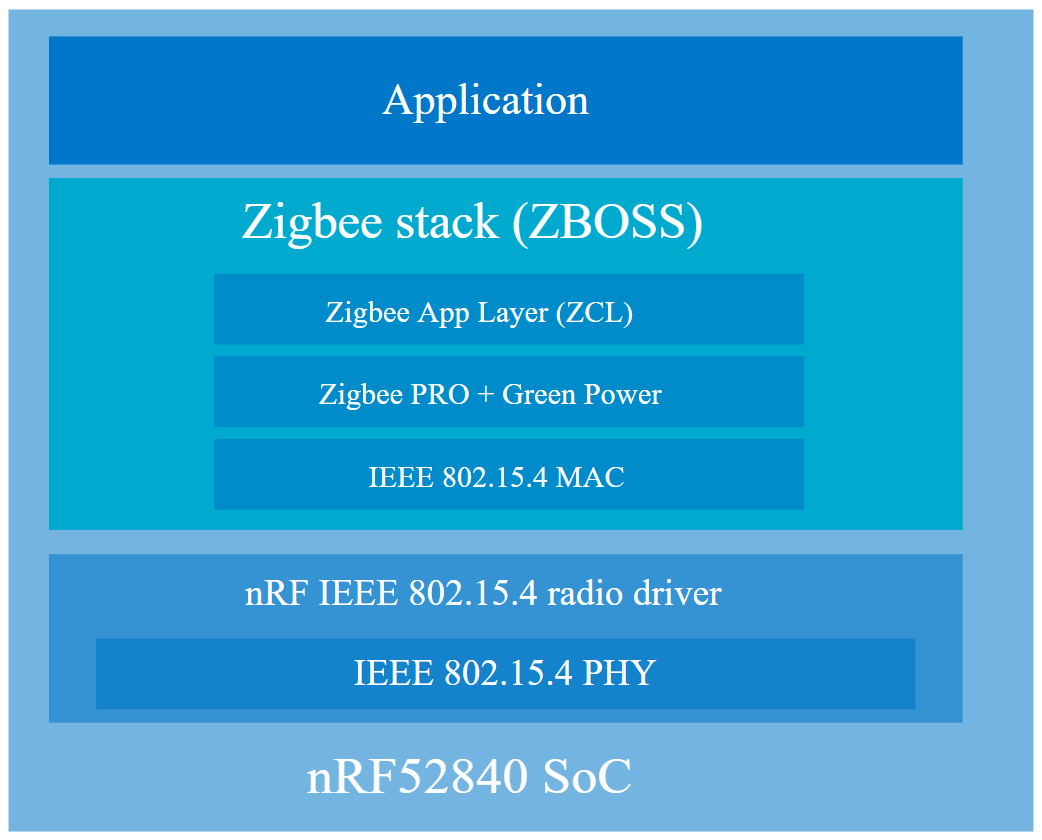
\includegraphics[width=0.6\textwidth]{Zigbee_SDK_Plattform_Design.png}
	\caption{nRF5 SDK for Thread and Zigbee Plattform Design Referenz \cite{nordic_semi_nrf_sdk_for_thread_and_zigbee_2020}}
	\label{fig:ZigbeePlattformDesign}
\end{figure}
 
\pagebreak

\clearpage
\section{Umsetzung Benchmark}\label{sec:UmsetzungBenchmark}
\todo[inline]{Komplette Beschreibung der Firmware unterteilt in die 3 Nodetypen. Besonderheiten herausstreichen und allfällige Schwierigkeiten aufzeigen.}



\subsection{Benchmark Message}\label{subsec:BenchmarkMessage}

\subsection{Zigbee Stack Implementation}\label{subsec:ZigbeeStackImplementation}

\subsubsection{Funkkanal Wahl im 2.4GHz ISM Band}\label{subsubsec:FunkkanalWahlim2.4GHzISMBand}

\begin{figure}[h]
	\centering
	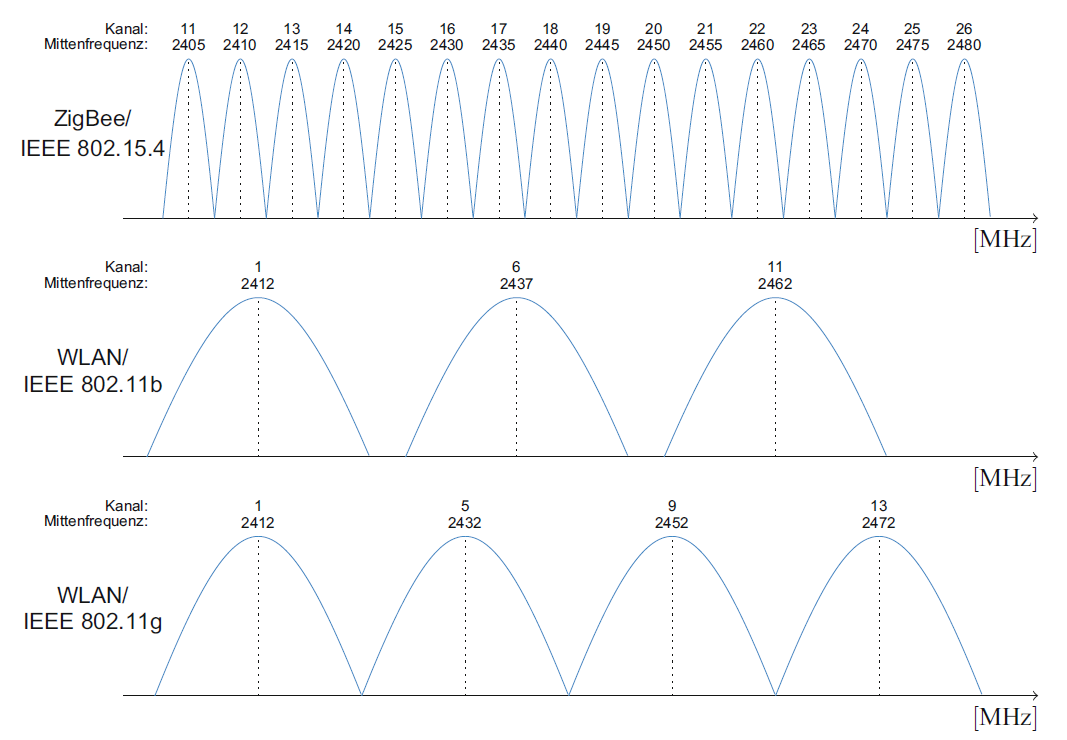
\includegraphics[width=\textwidth]{Funkkanaele_Konkurrenz_IEEE.png}
	\caption{Konkurrenz IEEE und WLAN Funkkanäle \cite{markus_krause_rainer_konrad_drahtlose_2014}}
	\label{fig:KonkurrenzIEEEundWLANFunkkanäle}
\end{figure}

\subsubsection{ZCL Level Cluster}\label{subsubsec:ZCLLevelCluster}

\subsubsection{Endpoint Handler}\label{subsubsec:EndpointHandler}

\subsubsection{APS Header}\label{subsubsec:Header}

\subsubsection{Adressierung}\label{subsubsec:Adressierung}


\pagebreak

\clearpage
\section{Analyse Zigbee Stack}\label{sec:AnalyseZigbeeStack}
Für die Umsetzung des Benchmark Konzepts war eine vertiefte Auseinandersetzung mit dem Zigbee Protokoll nötig.
Dabei konnten grosse Erfahrungen mit dem Stack sowie der verwendeten SDK gesammelt werden.
Aufgrund dieser Erfahrungen wird nachfolgend eine Analyse des Zigbee Protokollstacks sowie der eingesetzten SDK gemacht und einige Schwierigkeiten und Hindernisse bei der Softwareentwicklung aufgezeigt.

\subsection{Stärken und Schwächen des Protokollstacks}\label{subsec:ZigbeeStärkenundSchwächendesProtokollstacks}
Folgende Stärken und Schwächen weist der \textit{ZBOSS Zigbee Stack} auf.
Stack Implementationen von anderen Herstellern können nicht bewertet werden.

\textbf{Stärken:}
\begin{itemize}
\item Die \textbf{Zigbee Cluster Library (ZCL)} erleichtert die Umsetzung eines Produktes, welches mit anderen Zigbee Geräten konform sein soll erheblich.
\item Die \textbf{Adressierung mit Short-, Long- und Group-Adressen} ist übersichtlich und schlank gehalten.
Die vereinfacht das Handling für Entwickler und Anwender.
\item Ein simpler \textbf{Scheduler und Callback} Mechanismus vereinfacht das Nachrichten Handling.
\item Der \textbf{IEEE 802.15.4 Standard} für die MAC Ebene bietet dem Entwickler eine solide Basis um die gewünsche Anwendung darauf umsetzen zu können.
\end{itemize}

\textbf{Schwächen:}
\begin{itemize}
\item Bei der \textbf{Gruppen Adressierung} zeigt der Zigbee Stack deutliche Schwächen da für Broadcast Nachrichten ein kleinerer Packetbuffer verwendet wird.
\item Wenn \textbf{Zigbee Cluster Library (ZCL)} Funktionalitäten nicht zwingend benötigt werden, wird die Applikationsentwicklung umständlich.
Der Stack ist zu sehr auf vordefinierte Anwendungen ausgerichtet.
\item Die Spezifikationen des Stacks sind frei verfügbar. Leider implementieren die Hersteller den Stack schliesslich im \textbf{Closed-Source} Verfahren weshalb keine Community entstehen kann die den Stack verbessert.
\item Das \textbf{Commissioning} von neuen Teilnehmern hat in unserer Anwendung leider nicht immer reibungslos funktioniert.
Bei vielen gleichzeitigen Anmeldeanfragen kam der \textbf{Zigbee-Koordinator} gerne ins Straucheln und der Vorgang musste neu gestartet werden.
\end{itemize}


\subsection{Schwierigkeiten bei der Umsetzung}\label{subsec:ZigbeeSchwierigkeitenbeiderUmsetzung}
Einige Probleme haben die Entwicklung der Zigbee Benchmark Firmware schwieriger gemacht als erhofft.
Die folgenden 5 Punkte haben die Arbeiten merklich beeinflusst. 

\paragraph{Software Development Kit}
Da die \textit{nRF5 SDK for Thread and Zigbee} wohl bald von der \textit{nRF Connect SDK} abgelöst wird, scheint der Hersteller Nordic Semiconductor nicht wirklich Interesse daran zu haben, die \glqq alte\grqq{} SDK zu unterhalten.
Dies macht sich in der Dokumentation bemerkbar, denn gewisse API's sind nicht oder nur sehr schlecht dokumentiert.
Da es sich beim \textit{ZBOSS Zigbee Stack} um eine vorkompilierte Library handelt ist auch die Interpretation des Codes schwierig bis unmöglich.
In einigen Fällen verweist die Dokumentation sogar auf Funktionen und Beispiele die in der aktuellsten Version der SDK nicht mehr verfügbar sind.

\paragraph{Custom APS Data}
Die \textit{nRF5 SDK for Thread and Zigbee} bietet die Möglichkeit sogenannte \textit{Custom APS Data} zu versenden.
Dabei handelt es sich um eine Low Level API für den Versand von benutzerdefinierten Anwendungsdaten ohne dass die ZCL benutzt werden muss.
Während der Umsetzung des Benchmarks hat sich gezeigt, dass der Empfang und die Auswertung dieser Daten nur sehr schwierig umsetzbar ist.
Die entsprechende Dokumentation innerhalb der SDK war schlicht nicht ausreichend detailliert.
Im Benchmark Kontext hätte diese Funktion den Versand simpler Applikationsdaten vereinfacht.

\paragraph{Anzahl Hops}
Für die Auswertung der Messergebnisse in den Abschnitten \ref{sec:Messresultate} und \ref{sec:VergleichMeshNetzwerke} wurden unterschiedliche Messgrössen erfasst.
Unter anderem wäre auch die Anzahl Hops die eine Benchmark Nachricht innerhalb des Mesh Netzwerkes passiert hat, von grosser Wichtigkeit.
Nur so kann die Latenzzeit unabhängig von gewählten Weg definiert und mit den Latenzzeiten der anderen Protokolle verglichen werden.
Leider bietet die \textit{nRF5 SDK for Thread and Zigbee} keine Möglichkeit diesen Wert zu bestimmen, da das Radius-Feld aus dem NWK-Header nicht ausgelesen werden kann.
Das Radius-Feld wäre gemäss neuster \href{https://zigbeealliance.org/solution/zigbee}{Zigbee Specification\footnote{\url{https://zigbeealliance.org/solution/zigbee}\cite{the_zigbee_alliance_zigbee_2015}}} ein 8-Bit Feld im NWK-Header, welches beim passieren eines Hops dekrementiert wird \cite{the_zigbee_alliance_zigbee_2015}.
Das Paket wird verworfen sobald das Feld den Wert 0 erreicht.
Der folgende Beitrag aus dem Supportforum von Nordic Semiconductor bestätigt dieses Problem: \href{https://devzone.nordicsemi.com/f/nordic-q-a/63815/zigbee---read-number-of-hops-radius}{Zigbee - Read number of hops (radius)\footnote{\url{https://devzone.nordicsemi.com/f/nordic-q-a/63815/zigbee---read-number-of-hops-radius}\cite{cyrill_horath_zigbee_2020}}}





\paragraph{Group addressing mode}
Diverse Tests mit implementiertem \textit{ZCL groups cluster} haben gezeigt, dass Zigbee bei der Adressierung von Gruppenadressen schnell überfordert ist.
Selbst bei durchschnittlichem Verkehrsaufkommen im Netzwerk, konnte grosser Packetverlust von über 90 Prozent festgestellt werden.
Getestet wurde dies mit den Messreihen 1 und 2 gemäss Abschnitt \ref{subsec:Messreihe}.
Eine Gruppenadressierung löst in Zigbee eine Broadcast Nachricht aus, welche von allen Teilnehmern weitergeleitet wird.
Dies verursacht ein relativ grosses Verkehrsaufkommen im Netz. 
Es wird vermutet, dass der Paketbuffer für Broadcast Nachrichten zu klein ist und dieser zu langsam abgearbeitet wird.
Dadurch überläuft der Paketbuffer zu schnell und es entstehen die erwähnten Probleme.
Es konnte festgestellt werden, dass nach ca. 15 versendeten Nachrichten, keine weiteren Nachrichten zugestellt werden können, bis sich der Stack nach einiger Zeit wieder erholen konnte.

\paragraph{nRF Connect SDK}
Nordic Semiconductor stellt nebst der in dieser Arbeit verwendeten \textit{nRF5 SDK for Thread and Zigbee} noch eine weitere SDK für die Entwicklung von Zigbee Produkten zur Verfügung.
Die \textit{nRF Connect SDK} unterstützt seit der Version v1.3.0 ebenfalls den Zigbee Protokollstack.
Im Verlauf dieser Arbeit wurde auch diese SDK testweise eingesetzt.
Leider hat sich erst spät herausgestellt, dass die \textit{nRF Connect SDK} noch einige Kinderkrankheiten bei der Verwendung mit Zigbee besitzt.
So werden Nachrichten teilweise erst mit einer Verzögerung von 200ms versendet. In den \href{https://developer.nordicsemi.com/nRF_Connect_SDK/doc/1.3.0/nrf/doc/release-notes-1.3.0.html}{Release Notes\footnote{\url{https://developer.nordicsemi.com/nRF_Connect_SDK/doc/1.3.0/nrf/doc/release-notes-1.3.0.html}}} zu der entsprechenden Version ist dies festgehalten. 

\pagebreak



%%Part 4 Resultate und Validierung

\vspace*{4cm}
\part{Mesh Benchmark - Resultate und Vergleich}\label{part:MeshBenchmarkResultateundVergleich}
\vspace*{\fill}
\clearpage

\section{Messresultate}\label{sec:Messresultate}
Bei der Durchführung der Mesh Benchmark Messungen wurde für jede Messung unter den entsprechenden Bedingungen ein Messprotokoll resp. eine Auswertung erstellt. Die acht unterschiedlichen Bedingungen sind in Tabelle \ref{tab:MessungenMeshBenchmark} nochmals zusammengefasst sind.
Diese detaillierten Auswertungen sind im Anhang \ref{app:MessprotokolleMeshBenchmark} dem Bericht angefügt.
Nachfolgend wird exemplarisch eine dieser Auswertungen erläutert, um aufzuzeigen, was diese darstellen und wie diese gelesen werden können.
Eine Interpretation der Messresultate im Rahmen eines Vergleichs erfolgt anschliessend im Abschnitt \ref{sec:VergleichMeshNetzwerke}.

\begin{table}[h]
\centering
\begin{tabular}{|c|c|c|c|c|c|} 
\hline
\textbf{\#}  & \textbf{Msg. Gen.}  & \textbf{Duration}  & \textbf{Msg. Cnt.}  & \textbf{Payload }  & \textbf{Disturbance}  \\ 
\hline
1 & Rand & 600s & 60 & Small & No \\ 
\hline
2 & Seq & 600s & 60 & Small & No \\ 
\hline
3 & Rand & 600s & 60 & Large & No \\ 
\hline
4 & Seq & 600s & 60 & Large & No \\ 
\hline
5 & Rand & 600s & 600 & Small & No \\ 
\hline
6 & Rand & 600s & 60 & Small & Yes \\ 
\hline
7 & Seq & 750s & 10 & Small & No \\ 
\hline
8 & Seq & 750s & 10 & Large & No \\
\hline
\end{tabular}
\caption{Messbedingungen Mesh Benchmark}
\label{tab:MessungenMeshBenchmark}
\end{table}


\subsection{Resultate}\label{subsec:Resultate}
Die Messresultate im Anhang \ref{app:MessprotokolleMeshBenchmark} wurden mit den Messindizes 1-8 gemäss Tabelle \ref{tab:MessungenMeshBenchmark} sowie der entsprechenden Messumgebung (z.B. Wohnung) versehen.
So können die Messungen eindeutig identifiziert werden.
Folgende Einschränkungen müssen dabei jedoch beachtet werden:
Gemäss den Erläuterungen im Abschnitt \ref{subsec:Messreihe} wurden die Messungen 6 - 8 nur im Labor-Messaufbau durchgeführt. Von diesen Messungen sind dementsprechend auch nur diese drei Auswertungen vorhanden.
Weiter musste bei der Durchführung der Messung 5 festgestellt werden, dass die Resultate unbrauchbar waren.
Aus diesem Grund musste die Auswertung dieser Messung gestrichen werden.
Im Abschnitt \ref{subsec:Validierung} wird nochmals darauf eingegangen.

Die Abbildungen \ref{fig:VerteilungderLatenzzeiten} bis \ref{fig:OngoingTransactions} zeigen die Messresultate der Messung 2 in der Messumgebung \textit{Wohnung}. Sie stehen exemplarisch für die Messergebnisse aller Messreihen.
In Abbildung \ref{fig:VerteilungderLatenzzeiten} ist die prozentuale Verteilung der Latenzzeiten pro Hop dargestellt.
In sämtlichen Grafiken werden die Ergebnisse von BT Mesh in blau, jene von Thread in grün und jene von Zigbee in rot dargestellt.
Dadurch ist ein direkter Vergleich der Protokolle möglich.
Abbildung \ref{fig:VerteilungderLatenzzeiten} zeigt folglich, wie viele Nachrichten das Ziel mit einer bestimmten Latenzzeit erreicht haben.
Nachrichten, die das Ziel nicht erreicht haben, also Pakete die verloren gegangen sind, werden dabei nicht berücksichtigt. Diese werden jedoch als Paketloss aufgezeichnet. Im gezeigten Beispiel haben rund 76 Prozent der Nachrichten, die im BT Mesh Test versendet wurden, das Ziel mit einer maximalen Latenzzeit von 10 Millisekunden erreicht.
Die weitere Verteilung geht bis auf Latenzzeiten von über 300 Millisekunden, wobei die Prozentzahl der Nachrichten in diesem Bereich sehr tief ist.
Die Werte für Thread und Zigbee zeigen hingegen eine deutlich kleinere Verteilung der Latenzzeiten.

\begin{figure}[h]
	\centering
	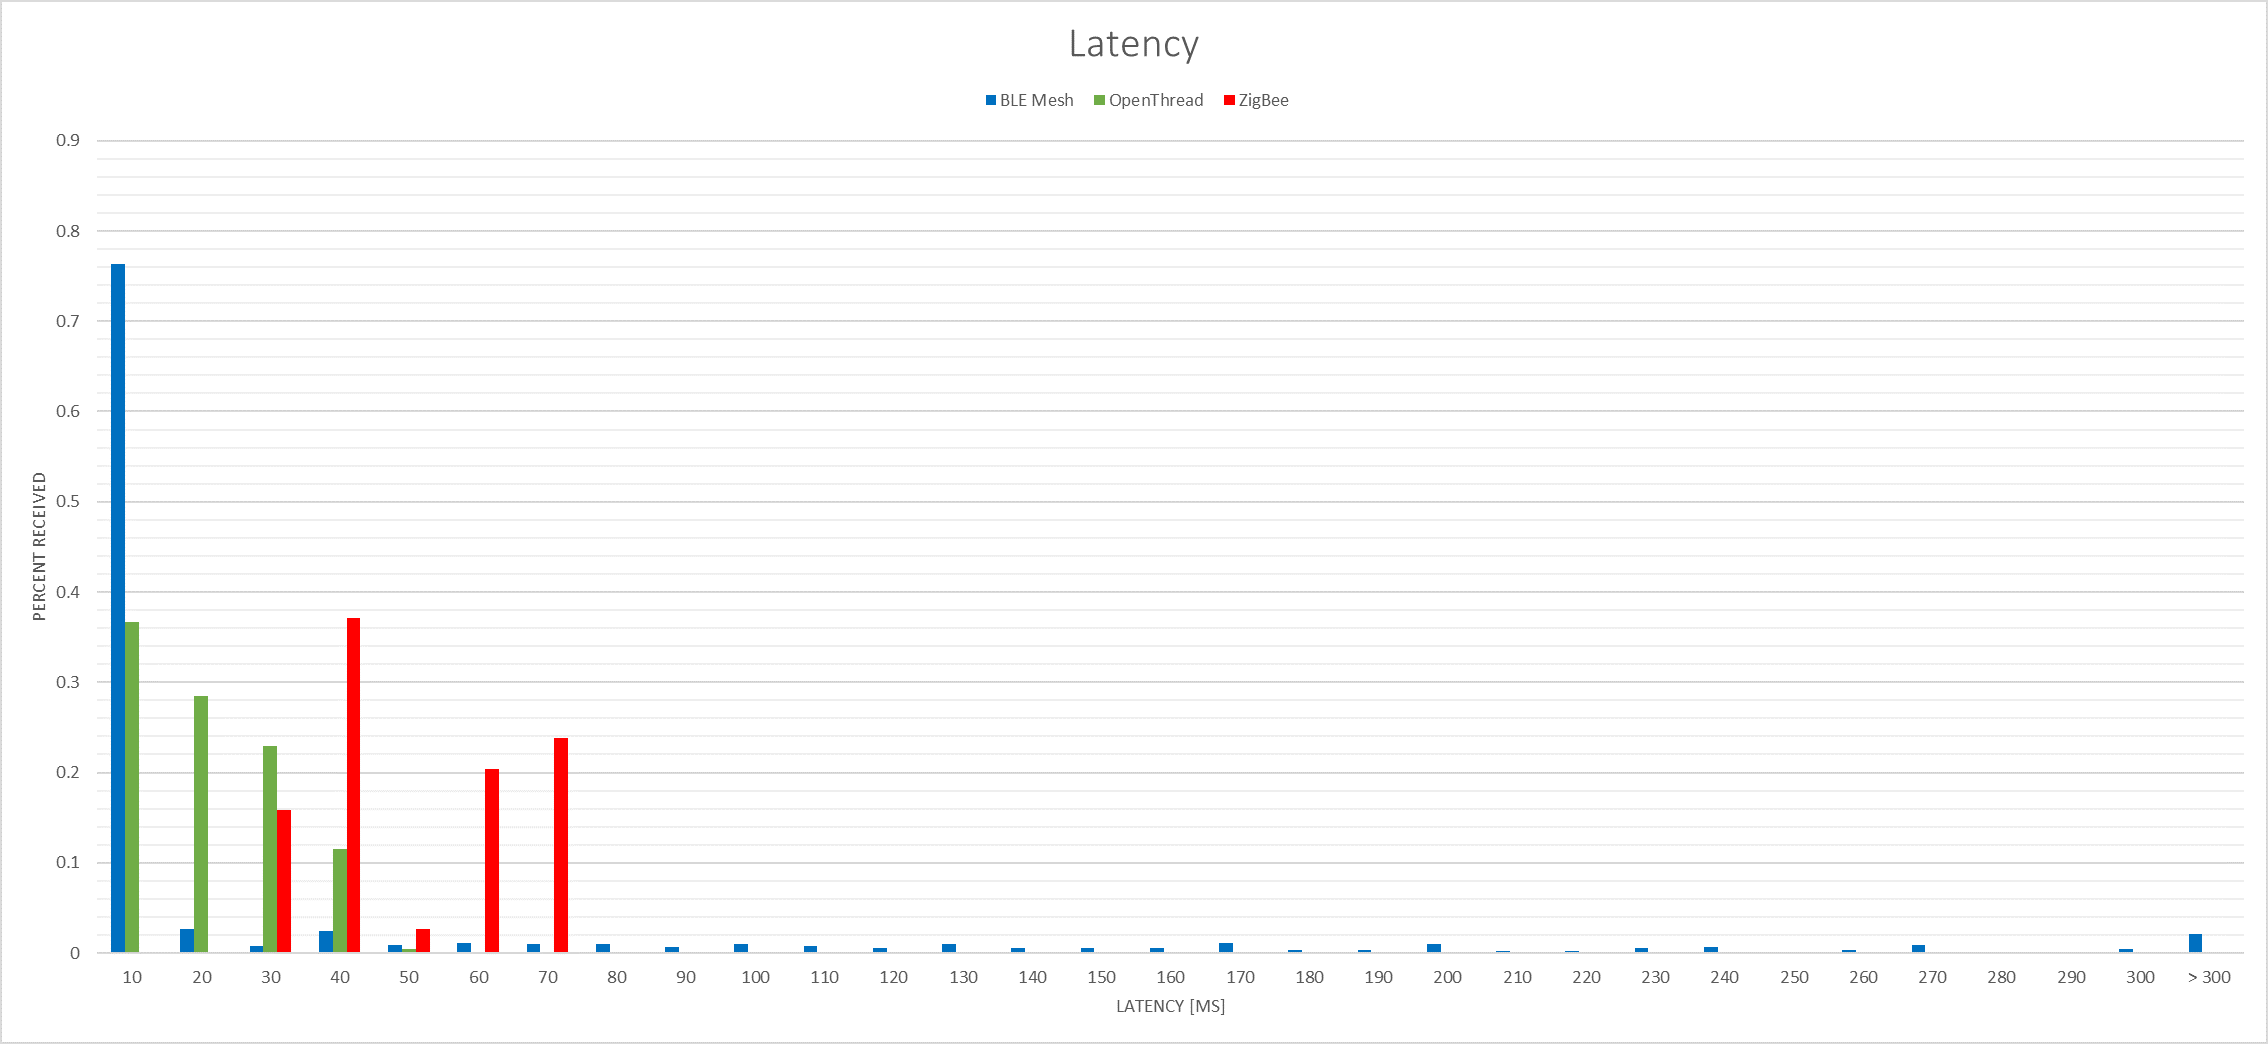
\includegraphics[width=\textwidth]{Latency_2_Wohnung.png}
	\caption{Messung 2 Wohnung: Verteilung der Latenzzeiten pro Hop}
	\label{fig:VerteilungderLatenzzeiten}
\end{figure}

Aus den in Abbildung \ref{fig:VerteilungderLatenzzeiten} aufgezeigten Latenzzeiten wurde der Durchschnitt über alle Messreihen gebildet und in Abbildung \ref{fig:DurchschnittlicheLatenzzeit} dargestellt.
Es handelt sich dabei wiederum um die Latenzzeit pro Hop. Im Falle von Zigbee ist dies erwähnenswert, da hier die Anzahl Hops nicht ausgelesen werden konnte (siehe Abschnitt \ref{subsec:ZigbeeSchwierigkeitenbeiderUmsetzung}) und die Resultate somit mit Vorsicht interpretiert werden müssen. Mehr dazu in der Validierung im Abschnitt \ref{subsec:Validierung}.

Der durchschnittliche Datendurchsatz, der in Abbildung \ref{fig:DurchschnittlicherDurchsatz} aufgezeigt wird, muss ebnfalls mit Vorsicht betrachtet werden. Denn auch hier werden die Werte pro Hop für die Berechnung verwendet.
Die präsentierten Werte werden aus der Paketgrösse (Small oder Large) gemäss den Definitionen in Abschnitt \ref{subsec:AllgemeineBenchmarkParameter} und der Latenzzeit des übertragenen Pakets (siehe Gleichung \ref{eq:BerechnungDurchsatz}), errechnet.
Dabei werden die Werte für den Durchsatz pro empfangenes Paket berechnet und davon schliesslich der Mittelwert gebildet.
Die oben erwähnten Ausreisser bei BT Mesh bewirken nun einen unerwartet hohen Durchsatz im Vergleich zu jenem bei Thread, das konstant tiefe Latenzzeiten aufweist.

\begin{equation}\label{eq:BerechnungDurchsatz}
TP =  \frac{S_{packet} \cdot 8}{t_{lat}}
\end{equation}

\begin{small}
\begin{center}
\begin{tabular}{ll}
$TP$ & Throughput (kBit/s)\\
$S_{packet}$ & Packetsize (Byte)\\
$t_{lat}$ & Latency time (ms)\\
\end{tabular}
\end{center}
\end{small}

\begin{figure}[!htbp]
\centering
\begin{minipage}[b]{0.49\textwidth}
		\centering
		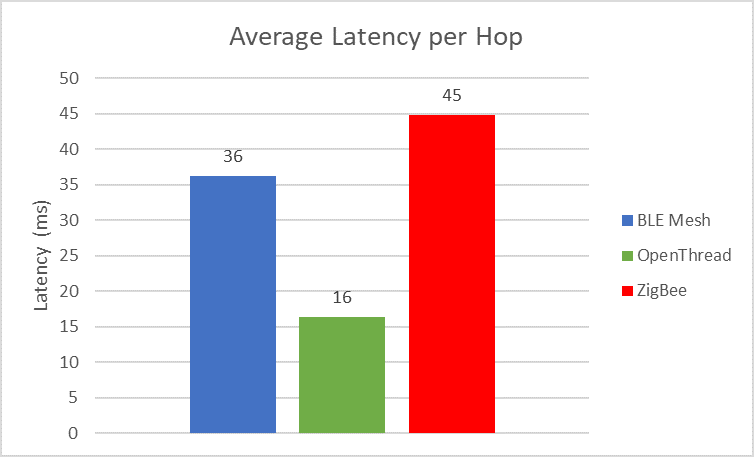
\includegraphics[width=\textwidth]{Average_Latency_per_Hop.png}
		\caption{Messung 2 Wohnung: Durchschnittliche Latenzzeit pro Hop}
		\label{fig:DurchschnittlicheLatenzzeit}
\end{minipage}
\begin{minipage}[b]{0.49\textwidth}
		\centering
		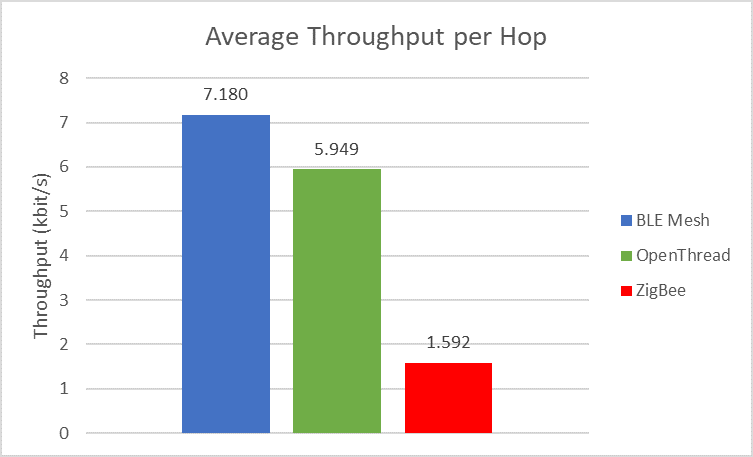
\includegraphics[width=\textwidth]{Average_Throughput_per_Hop.png}
		\caption{Messung 2 Wohnung: Durchschnittlicher Durchsatz pro Hop}
		\label{fig:DurchschnittlicherDurchsatz}
\end{minipage}
\end{figure}

In Abbildung \ref{fig:DurchschnittlicherPaketverlust} wird der Paketverlust im Verhältnis zur gesamten Anzahl Nachrichten, die während dem Benchmark versendet wurden, in Prozenten aufgezeigt.
Die Paketverluste von einzelnen Client-Server Beziehungen werden nicht separat ausgewertet.
Wiederum im Beispiel von BT Mesh sind in dieser Messung 2.07 \% der Pakete nicht am Ziel angekommen.

\begin{figure}[!htbp]
\centering
\begin{minipage}[b]{0.49\textwidth}
		\centering
		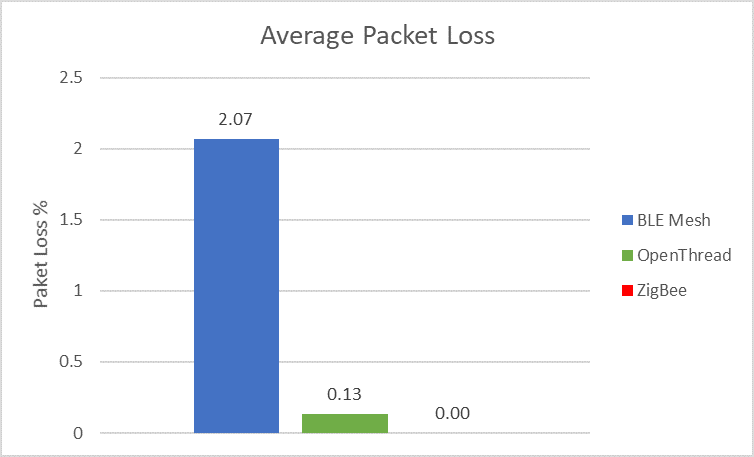
\includegraphics[width=\textwidth]{Average_Packet_Loss.png}
		\caption{Messung 2 Wohnung: Durchschnittlicher Paketverlust}
		\label{fig:DurchschnittlicherPaketverlust}
\end{minipage}
\begin{minipage}[b]{0.49\textwidth}
		\centering
		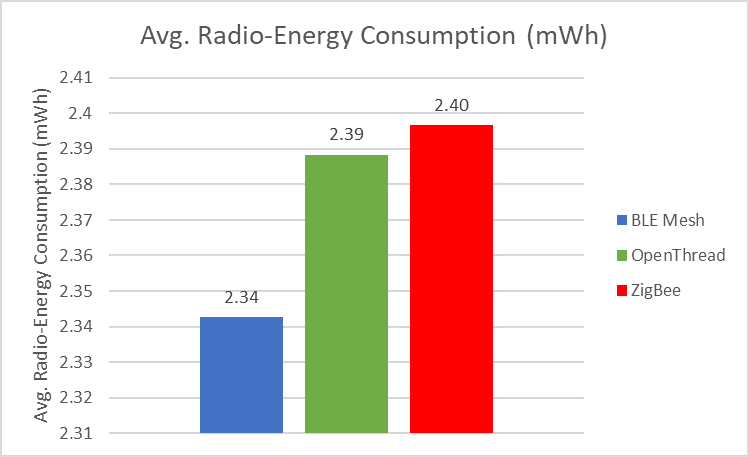
\includegraphics[width=\textwidth]{Average_Radio_Energy_Consumption.png}
		\caption{Messung 2 Wohnung: Durchschnittlicher Energieverbrauch}
		\label{fig:DurchschnittlicherEnergieverbrauch}
\end{minipage}
\end{figure}

Mit dem Diagramm in Abbildung \ref{fig:DurchschnittlicherEnergieverbrauch} wird schliesslich noch der durchschnittliche Energieverbrauch der Protokolle dargestellt.
Dieser wird abgeleitet aus der \textit{Active Radio Time} (siehe Abschnitt \ref{subsubsec:Vergleichswerte}), welche direkt auf dem nRF52840 SoC mit der entsprechenden API ausgelesen werden kann.
Die \textit{Active Radio Time} wurde schliesslich mit dem Strombedarf des SoC's bei definierter Speisespannung von 3V verrechnet.
Gemäss den Angaben in Tabelle \ref{tab:EigenschaftennRF52840SoC} aus Abschnitt \ref{subsec:SystemonChip} beträgt der Strombedarf bei aktivem Funkmodul im Sendemodus 4.8mA.
Eine solche Berechnung erlaubt einen qualitativen Vergleich des Energiebedarfs unter den drei Protokollen, da die Umsetzung auf der gleichen Hardware erfolgte.
Die Werte in Abbildung \ref{fig:DurchschnittlicherEnergieverbrauch} sind jedoch keine quantitativen Verbrauchswerte und können deshalb nur im Kontext des Vergleichs verwendet werden.
Der Strombedarf sämtlicher Peripherie wurde nicht berücksichtigt, da dieser prinzipiell bei allen Protokollen identisch und in diesem Fall daher nicht interessant ist.

\begin{figure}[h]
	\centering
	\includegraphics[width=\textwidth]{Ongoing_Transactions_and_Latency.png}
	\caption{Messung 2 Wohnung: Ongoing Transactions und Verlauf der Latenzzeiten über die Messdauer.}
	\label{fig:OngoingTransactions}
\end{figure}

Die letzte Grafik gemäss Abbildung \ref{fig:OngoingTransactions} zeigt den Verlauf der \textit{Ongoing Transactions} sowie der Latenzzeiten über die Gesamtdauer einer Messung.
In diesem Fall beträgt die Dauer 600 Sekunden.
Die Grafik soll einen Eindruck darüber vermitteln, wie die Stacks damit umgehen, wenn vielen Nachrichten zur selben Zeit versendet werden.
Die \textit{Ongoing Transactions}, welche als durchgezogene Linien dargestellt sind, zeigen zu welchem Zeitpunkt wie viele Nachrichten im Übermittlungsprozess sind.
Da die Nachrichten in diesem Beispiel sequentiell versendet werden, gibt es nur sehr geringe Ausschläge, welche im unteren Bildrand der Abbildung \ref{fig:OngoingTransactions} zu sehen sind.
Die logarithmische Darstellung der Latenzzeiten als gestrichelte Linie bestätigt die Beobachtungen, die in Abbildung  \ref{fig:VerteilungderLatenzzeiten} bereits gemacht wurden.
Zigbee und Thread weisen einen ziemlich regelmässigen Verlauf der Latenzzeiten auf.
BT Mesh hingegen zeigt starke Ausreisser.

\subsection{Validierung}\label{subsec:Validierung}
Die durchgeführten Messungen haben aussagekräftige Resultate geliefert, welche jedoch stark vom gewählten Vorgehen abhängig sind.
Dieses Vorgehen wird nun kritisch überprüft und allfällige Mängel im Konzept sowie in der Umsetzung werden aufgezeigt.
Zudem werden systematische Messfehler deklariert.

\paragraph{Large Payload}
Die Messungen 3, 4 und 8 gemäss Tabelle \ref{tab:MessungenMeshBenchmark}, welche mit einer grossen Payload durchgeführt wurden, sind nur für Thread und Zigbee aussagekräftig. Der BT Mesh Stack liefert bei diesen Messungen keine brauchbaren Resultate.
Eine Recherche zu diesem Problem hat ergeben, dass durch die Fragmentierung einer 32 Byte Payload die sichere und schnelle Übertragung der Daten nicht mehr gewährleistet werden kann. Dieses Problem wird in Abschnitt \ref{subsec:BLEMeshProtokollStackZephyr} genauer erläutert.

\paragraph{Zigbee Latency}
Wie bereits im Abschnitt \ref{subsec:ZigbeeSchwierigkeitenbeiderUmsetzung} erwähnt, konnte bei Zigbee die Anzahl Hops, die ein Paket passiert hat nicht ausgewertet werden.
Der Forumsbeitrag \href{https://devzone.nordicsemi.com/f/nordic-q-a/63815/zigbee---read-number-of-hops-radius}{\textit{Zigbee - Read number of hops (radius)\footnote{\url{https://devzone.nordicsemi.com/f/nordic-q-a/63815/zigbee---read-number-of-hops-radius}}}} bestätigt, dass der entsprechende Wert mit der verwendeten SDK nicht ausgelesen werden kann.
Die Folge davon ist, dass die Latenzzeit nur als Total über die gesamte Strecke erfasst werden kann.
In der Auswertung verschafft dies fälschlicherweise BT Mesh und Thread einen Vorteil gegenüber Zigbee.
Die Auswertung der totalen Latenzzeit bei allen drei Protokollen könnte das Problem lösen.
Dies würde jedoch dem Messkonzept widersprechen und wurde deshalb nicht für alle Messungen umgesetzt.
Die Abbildungen \ref{fig:DurchschnittlicheLatenzzeitValidierung} und \ref{fig:DurchschnittlicheLatenzzeitohneHopsValidierung} zeigen den Unterschied am Beispiel der oben analysierten Messung im Abschnitt \ref{subsec:Resultate}.
Während in Abbildung \ref{fig:DurchschnittlicheLatenzzeitValidierung} die Latenzzeit pro Hop dargestellt ist, zeigt die Abbildung \ref{fig:DurchschnittlicheLatenzzeitohneHopsValidierung} die totale Latenzzeit.
Der Unterschied ist vorallem bei Thread deutlich erkennbar.
Bereits in Abbildung \ref{fig:VerteilungderLatenzzeiten} ist diese Problematik zu erahnen.
Denn die Statistik der Latenzzeiten von Zigbee zeigt zwei Hauptsäulen bei 40ms und 70ms. Dies deutet darauf hin, dass die Pakete mit 70ms Latenzzeit einen Hop passiert haben und jene bei 40ms nicht.


\begin{figure}[!htbp]
\centering
\begin{minipage}[b]{0.49\textwidth}
		\centering
		\includegraphics[width=\textwidth]{Average_Latency_per_Hop.png}
		\caption{Durchschnittliche Latenzzeit pro Hop}
		\label{fig:DurchschnittlicheLatenzzeitValidierung}
\end{minipage}
\begin{minipage}[b]{0.49\textwidth}
		\centering
		\includegraphics[width=\textwidth]{Average_Latency_without_Hops.png}
		\caption{Durchschnittliche Latenzzeit ohne Berücksichtigung der Hops.}	\label{fig:DurchschnittlicheLatenzzeitohneHopsValidierung}
\end{minipage}
\end{figure}

\paragraph{Nachrichten Dichte}
Bei der Definition der Messreihen \ref{subsec:Messreihe} wurden zu Beginn nur die Messungen 1 bis 6 spezifiziert.
Die Messreihen 7 und 8 kamen erst nachträglich hinzu, als festgestellt werden musste, dass die Dichte der Nachrichten für den BT Mesh Stack zu hoch gewählt wurde.
Der BT Mesh Stack war überfordert beim Empfang von zufällig generierten Nachrichten, wie im Abschnitt \ref{subsec:TrafficGeneration} beschrieben ist.
Thread und Zigbee zeigten indes keine Mühe mit der Dichte von 60 Nachrichten in 600 Sekunden pro Node.
Die Resultate der Messungen 7 und 8 haben schliesslich gezeigt, dass die Reduktion der Nachrichtendichte einen positiven Einfluss auf die Performance von BT Mesh hat.

Die Messung Nummer 5 wurde aufgrund der selben Problematik aus den Auswertungen gestrichen. 
Hier wäre die Dichte der Nachrichten um das zehnfache grösser gewesen als bei der vergleichbaren Messung mit dem Index 1.
Eine Auswertung der Messdaten wäre daher sinnlos gewesen.

\paragraph{Group addressing mode}
Der \textit{Group addressing mode} wurde im Abschnitt \ref{subsec:AllgemeineBenchmarkParameter} für die drei Protokolle unterschiedlich definiert.
Erste Tests vor den eigentlichen Benchmarks haben gezeigt, dass eine Multicast Adressierung bei Zigbee unbrauchbar ist (siehe Abschnitt \ref{subsec:ZigbeeSchwierigkeitenbeiderUmsetzung}).
Deshalb hat man sich entschieden, bei Zigbee eine Unicast Adressierung umzusetzen.
Während den Benchmarks musste schliesslich festgestellt werden, dass Zigbee durch diese Änderung einen wesentlichen Vorteil erlangt hat.
Besonders auf die Paketverlustrate hat sich die Unicast Adressierung positiv ausgewirkt, denn Unicast Nachrichten verursachen deutlich weniger Verkehr innerhalb des Netzwerkes als Broadcast Nachrichten.

Auch in der Messung Nr. 5 hätte sich die Unicast Adressierung für Zigbee positiv ausgewirkt, da die Netzbelastung deutlich geringer gewesen wäre.
 
\paragraph{Durchschnittswerte in den Resultaten}
In den Resultaten \ref{subsec:Resultate} wurden sämtliche Durchschnittswerte als Mittelwerte einschliesslich allfälliger Ausreisser aus den Messwerten gebildet.
Dadurch wurden gewisse Resultate deutlich verfälscht.
In einer verbesserten Auswertung müsste die Ursache für die einzelnen Ausreisser genauer geklärt werden und diese allenfalls gestrichen werden. Zudem müsste für eine bessere Auswertung der Median bestimmt werden, um allfällige Ausreisser zu kompensieren.
Dies wurde leider zu spät entdeckt und konnte daher nicht umgesetzt werden.


\subsection{Verifizierung}\label{subsec:Verifizierung}
Eine Verifizierung der Messresultate konnte nur anhand des Referenzberichts \textit{AN1142: Mesh Network Performance
Comparison\footnote{\url{https://www.silabs.com/documents/public/application-notes/an1142\%2Dmesh\%2Dnetwork\%2Dperformance\%2Dcomparison.pdf} \cite{silicon_laboratories_inc_an1142_2020}}} von \textit{Silicon Labs} gemacht werden.
Dieser ist auf der Webseite von \textit{Silicon Labs} einsehbar.

Der Vergleich der Messergebnisse hat gezeigt, dass die Grössenordnung der Resultate mit jenen aus dem Bericht von Silicon Labs übereinstimmt.
Selbst die Ausreisser in der Latenzzeit bei BT Mesh liegen im selben Rahmen.
Zudem kann die klare Abhängigkeit der Resultate von der Grösse der Payload bestätigt werden.
Einige Unterschiede sind jedoch in der Verteilung der Latenzzeiten erkennbar.
Im Referenzbericht ist diese in einem Bereich zwischen 20ms und 60ms ziemlich regelmässig, während in den Ergebnissen dieser Thesis die Verteilung unregelmässiger daherkommt.







\pagebreak

\clearpage

\section{Validierung}\label{sec:Validierung}
\todo[inline]{Einschätzung und Überprüfung der Richtigkeit der Messungen.}

\subsection{Vergleich Mesh Protokolle}\label{sec:VergleichMeshProtokolle}
\todo[inline]{Wie gut können die Mesh Protokolle überhaupt verglichen werden? Wo sind sie Protokolle zu sehr unterschiedlich?}

\subsection{Zeitsynchronisation}\label{sec:Zeitsynchronisation}
\todo[inline]{Genauigkeit der Zeitsynchronisation im Mesh und/oder P2P.}

\subsection{Messwerte}\label{sec:Messwerte}
\todo[inline]{Auflistung der Genauigkeiten resp. Fehler pro Messwert. Systematische und statistische Fehler.}

\subsection{Auswertung der Messwerte}\label{sec:AuswertungderMesswerte}
\todo[inline]{Fehler die während der Auswertung entstanden sind.}

\subsection{Konzept}\label{sec:Konzept}
\todo[inline]{Wurden bei der Kozeptionierung systematische Fehler gemacht die nicht eliminiert werden konnten?}
\pagebreak

\clearpage

\section{Schluss}\label{sec:Schluss}


\subsection{Zielerreichung}\label{subsec:Zielerreichung}
Für die vorliegende Projektarbeit wurden im Pflichtenheft (siehe Anhang \ref{app:Pflichtenheft}) klare Ziele definiert. In den Tabellen \ref{tab:ErreichungP2PZiele}, \ref{tab:ErreichungMeshZiele}, \ref{tab:ErreichungSteuersoftwareZiele} und \ref{tab:ErreichungZusatzziele} sind diese in kurzer Form nochmals zusammengefasst. Ausserdem ist ersichtlich welche Ziele erfüllt werden konnten und welche nicht oder nur bedingt erfüllt sind.
Falls nötig ist auch noch ein kurzer Kommentar hinterlegt.

\todo[inline]{Raffi bitte P2P-Tabelle kontrollieren und ergänzen} 
\paragraph{Punkt zu Punkt Testinfrastruktur}
\begin{table}[H]
	\centering
	\begin{tabular}{|c|l|c|l|} 
		\hline
		\multicolumn{4}{|l|}{\textbf{Projektziele}}                                                                                                                                                                                                                                                                                                      \\ 
		\hline
		\textbf{Nr.}              & \textbf{Ziel}                                                                                      & \textbf{Erfüllt} & \textbf{Kommentar}                                                                                                                                                                           \\ 
		\hline
		P1                        & Kommunikation mit BMS                                                                              & Ja               & \begin{tabular}[c]{@{}l@{}}Alle Master Module werden via USB UART \\angesteuert.\end{tabular}                                                                                                \\ 
		\hline
		P2                        & Senden von MAC Frames                                                                              & Ja               &                                                                                                                                                                                              \\ 
		\hline
		P3                        & \begin{tabular}[c]{@{}l@{}}Rückbestätigung der \\MAC-Frames\end{tabular}                           & Ja               &                                                                                                                                                                                              \\ 
		\hline
		P4                        & \begin{tabular}[c]{@{}l@{}}Konfiguration der \\Anzahl BSN\end{tabular}                             & Bedingt          & \begin{tabular}[c]{@{}l@{}}Alle Slave-Nodes werden automatisch erkannt \\und angezeigt.\end{tabular}                                                                                         \\ 
		\hline
		P5                        & Adressierung der BSN                                                                               & Bedingt          & \begin{tabular}[c]{@{}l@{}}Alle Slave-Nodes werden automatisch erkannt \\und angezeigt.\end{tabular}                                                                                         \\ 
		\hline
		P6                        & Konfiguration der Kanäle                                                                           & Ja               & Kann über den Webserver angepasst werden.                                                                                                                                                    \\ 
		\hline
		P7                        & Einstellbare Framelänge                                                                            & Ja               & \begin{tabular}[c]{@{}l@{}}Die Payload kann über den Webserver \\eingestellt werden.\end{tabular}                                                                                            \\ 
		\hline
		P8                        & \begin{tabular}[c]{@{}l@{}}Einstellbare Frame und \\Kanalwechselrate\end{tabular}                  & Nein             &                                                                                                                                                                                              \\ 
		\hline
		P9                        & Einstellbare Sendeleistung                                                                         & Ja               & Kann über den Webserver angepasst werden.                                                                                                                                                    \\ 
		\hline
		\multicolumn{1}{|l|}{P10} & \begin{tabular}[c]{@{}l@{}}Anpassung der \\Modulationsart\end{tabular}                             & Ja               & Kann über den Webserver angepasst werden.                                                                                                                                                    \\ 
		\hline
		\multicolumn{1}{|l|}{P11} & \begin{tabular}[c]{@{}l@{}}Ein- und Ausschalten der \\Collision Avoidance \\(CSMA/CA)\end{tabular} & Ja               & \begin{tabular}[c]{@{}l@{}}Kann über den Webserver ein- und \\ausgeschaltet werden.\end{tabular}                                                                                             \\ 
		\hline
		\multicolumn{1}{|l|}{P12} & \begin{tabular}[c]{@{}l@{}}Erfassen der \\Verbindungsqualität\end{tabular}                         & Ja               & \begin{tabular}[c]{@{}l@{}}Der Master sendet und empfängt in einem \\Zeit Intervall Frames von den Slave-Nodes \\und sendet die Daten an die \\Serielle-Schnittstellt weiter.~\end{tabular}  \\ 
		\hline
		\multicolumn{1}{|l|}{P13} & Tool für Feldtests                                                                                 & Ja               & \begin{tabular}[c]{@{}l@{}}Das Tool ist mit dem Webserver und der \\Firmware einsatzbereit.\end{tabular}                                                                                     \\
		\hline
	\end{tabular}
	\caption{Erreichung der Ziele zur Punkt zu Punkt Testinfrastruktur}
	\label{tab:ErreichungP2PZiele}
\end{table}

\newpage
\paragraph{Test Mesh Netzwerke}
\begin{table}[H]
	\centering
	\begin{tabular}{|c|l|c|l|} 
		\hline
		\multicolumn{4}{|l|}{ \textbf{Projektziele} }                                                                                                                                                                                                                                                                   \\ 
		\hline
		\textbf{Nr.}  & \textbf{Ziel}                                                               & \textbf{Erfüllt}  & \textbf{Kommentar}                                                                                                                                                                            \\ 
		\hline
		P1            & Kommunikation mit BMS                                                       & Ja                & \begin{tabular}[c]{@{}l@{}}Alle Master Module werden via USB UART \\angesteuert.\end{tabular}                                                                                                 \\ 
		\hline
		P2            & Konfiguration BSN                                                           & Nein              & \begin{tabular}[c]{@{}l@{}}Alle Nodes im Netzwerk fungieren als \\Routing-Knoten.\end{tabular}                                                                                                \\ 
		\hline
		P3            & Mesh-Netzwerk                                                               & Ja                & \begin{tabular}[c]{@{}l@{}}Alle Netzwerke wurden in einem 50 Node \\Mesh-Netzwerk getestet.\end{tabular}                                                                                      \\ 
		\hline
		P4            & Simulation Sensorwerte                                                      & Ja                & \begin{tabular}[c]{@{}l@{}}Über ein Python Programm können \\Testzeit und Anzahl Nachrichten konfiguriert \\werden. Es können sogar verschiedene \\Zufalls-Modi gewählt werden.\end{tabular}  \\ 
		\hline
		P5            & Sensordaten                                                                 & Ja                & \begin{tabular}[c]{@{}l@{}}Die Sensordaten werden im RAM und \\FLASH des SoCs gespeichert und nach \\der Messung an den Master gesendet.\end{tabular}                                         \\ 
		\hline
		P6            & Datenauswertung                                                             & Ja                & \begin{tabular}[c]{@{}l@{}}Die Daten der Messungen wurden mit \\Hilfe~ von Excel Tabellen ausgewertet.\end{tabular}                                                                           \\ 
		\hline
		P7            & Störimmunität                                                               & Ja                & \begin{tabular}[c]{@{}l@{}}Störmessungen mit der \\P2P-Testinfrastruktur wurden gemacht.\end{tabular}                                                                                         \\ 
		\hline
		P8            & \begin{tabular}[c]{@{}l@{}}Unterschiedliche Test \\Bedingungen\end{tabular} & Ja                & \begin{tabular}[c]{@{}l@{}}Es wurden drei Bereiche getestet. \\Haus, Wohnung und Labor.\end{tabular}                                                                                          \\ 
		\hline
		P9            & Test und Validierung                                                        & Ja                & \begin{tabular}[c]{@{}l@{}}Die Mesh Netzwerke wurden im \\Fachbericht vollumfänglich verglichen \\und ausgewertet.\end{tabular}                                                               \\
		\hline
	\end{tabular}
	\caption{Erreichung der Ziele zu den Test Mesh Netzwerken}
	\label{tab:ErreichungMeshZiele}
\end{table}

\paragraph{Steuer- und Auswertesoftware}
\begin{table}[H]
	\centering
	\begin{tabular}{|c|l|c|l|} 
		\hline
		\multicolumn{4}{|l|}{ \textbf{Projektziele} }                                                                                                                                                                                                                                                                                \\ 
		\hline
		\textbf{Nr.}  & \textbf{Ziel}                                                                & \textbf{Erfüllt}  & \textbf{Kommentar}                                                                                                                                                                                        \\ 
		\hline
		P1            & Ansteuerung Funkmodul                                                        & Ja                & \begin{tabular}[c]{@{}l@{}}Alle Master Module werden via USB UART \\angesteuert.\end{tabular}                                                                                                             \\ 
		\hline
		P2            & Visualisierung Parameter                                                     & Bedingt           & \begin{tabular}[c]{@{}l@{}}Für die P2P-Testinfrastruktur steht ein \\Webserver zur Verfügung. Die Daten des \\Mesh-Tests werden erst in einer Excel \\Tabelle ausgewertet und Visualisiert.\end{tabular}  \\ 
		\hline
		P3            & User Interface (UI)                                                          & Ja                & \begin{tabular}[c]{@{}l@{}}Ein Django Webserver stellt ein UI für die \\Verwaltung der P2P-Testinfrastruktur \\zur Verfügung.\end{tabular}                                                                \\ 
		\hline
		P4            & \begin{tabular}[c]{@{}l@{}}Konfiguration Mesh-\\Netzwerk\end{tabular}        & Ja                & \begin{tabular}[c]{@{}l@{}}Ein Python Programm konfiguriert die \\Mesh Nodes über den BMN.\end{tabular}                                                                                                   \\ 
		\hline
		P5            & \begin{tabular}[c]{@{}l@{}}Einheitliche \\Kommunikation von BMS\end{tabular} & Ja                & \begin{tabular}[c]{@{}l@{}}Ein Python Programm steuert die Mesh \\Nodes über den BMN.\end{tabular}                                                                                                        \\
		\hline
	\end{tabular}
	\caption{Erreichung der zur Steuer- und Auswertesoftware}
	\label{tab:ErreichungSteuersoftwareZiele}
\end{table}

\paragraph{Zusatzziele}
\begin{table}[H]
	\centering
	\begin{tabular}{|c|l|c|l|} 
		\hline
		\multicolumn{4}{|l|}{ \textbf{Projektziele} }                                                                                                                                                                                                                  \\ 
		\hline
		\textbf{Nr.}  & \textbf{Ziel}                                                       & \textbf{Erfüllt}  & \textbf{Kommentar}                                                                                                                                   \\ 
		\hline
		P1            & \begin{tabular}[c]{@{}l@{}}Hardware Testmodul\\BMN/BSN\end{tabular} & Nein              & \begin{tabular}[c]{@{}l@{}}Mit Absprache der Coaches, ist ein \\Hardwaremodul nicht notwendig.\end{tabular}                                          \\ 
		\hline
		P2            & Vergleich SoC                                                      & Bedingt           & \begin{tabular}[c]{@{}l@{}}Die Bluetooth Tests wären mit verschiedenen \\SoCs möglich, diese Messungen wurden aber \\nicht ausgeführt.\end{tabular}  \\ 
		\hline
		P3            & Drahtlos Konfiguration                                              & Nein              & \begin{tabular}[c]{@{}l@{}}Ein Firmware over the air upgrade wurde \\nicht umgesetzt.\end{tabular}                                                   \\ 
		\hline
		P4            & UI für Mesh Test                                                    & Nein              & \begin{tabular}[c]{@{}l@{}}Für die Mesh-Tests wurde kein aus zeitlichen \\Gründen kein User-Interface geschrieben\end{tabular}                       \\
		\hline
	\end{tabular}
	\caption{Erreichung der Zusatzziele}
	\label{tab:ErreichungZusatzziele}
\end{table}


\newpage
\subsection{Fazit}\label{subsec:Fazit}
In dieser Arbeit wurden die drei Mesh Protokolle Bluetooth Mesh, Thread und Zigbee unter verschiedenen Testszenarien ausgemessen und anschliessend miteinander verglichen.
Wichtig zu verstehen ist, dass es kein bestes Mesh Netzwerk gibt.
Alle Protokolle haben ihre Stärken und Schwächen in verschiedenen Umgebungen und mit verschiedenen Messparametern.
Nachfolgend wird zusammengefasst, welche Schlüsse aus dem Vergleich der drei Protokollen gezogen worden sind.

\begin{itemize}

	\item Bluetooth Mesh hat den grössten Vorteil in einer Umgebung, bei der sich die Knoten stetig bewegen. Dies aus dem Grund, dass das Mesh keine Routing Knoten verwendet.
	\item Der grösste Vorteil von Thread ist es, dass sich das Mesh-Netzwerk selber ausmisst. Die routenden Knoten werden automatisch bestimmt. Somit kann sich das Protokoll der Umgebung anpassen und konnte dadurch auch in allen Testumgebungen eine tiefe Latenz zu Tage legen.
	\item Ein Nachteil von Thread ist es, dass wegen dem automatischen Routen ein höherer Overhead entsteht. Durch diesen Overhead steigt der Energieverbrauch auf den einzelnen Nodes
	\item Zigbee weist eine hohe Zuverlässigkeit auf.
	Bedingt durch das CSMA\slash CA des\linebreak \textit{IEEE 802.15.4} MAC und Physical Layer erreichen weit mehr als 95 Prozent der Nachrichten ihr Ziel mit konstant tiefer Latenzzeit.
	\item Der gemessene Durchsatz und die gemessene Latenzzeit kann nicht ganz mit jenen Werten von Thread mithalten.
	Daher ist die Performance bei hoher Belastung eher schlechter.
		\item \todo[inline]{Ein Vorteil und ein Nachteil erwähnen pro Mesh-Stack. Raffel bitte noch ausfüllen}
\end{itemize}

Nachfolgend wird auf einige Probleme eingegangen welche während dem Projekt entstanden sind. Ausserdem werden mögliche Lösungen dafür vorgeschlagen.
Die Probleme werden in organisatorische und technische Verbesserungsvorschläge aufgeteilt.

\textbf{Organisatorische Verbesserungen}
\begin{itemize}
	\item Ein frühzeitiges Softwarekonzept hätte sehr viel Redundanz in der verschiedenen Firmware Teilen erspart und somit auch viel Zeit eingespart.
	\item Die Arbeitsaufteilung müsste besser kommuniziert und besprochen werden, ansonsten wird der Arbeitsaufwand für die jeweiligen Personen ungerecht aufgeteilt.
\end{itemize}

\textbf{Technische Verbesserungen}
\begin{itemize}
	\item Durchschnittswerte sollten mit dem Median bestimmen werden. Der momentane Mittelwert wird zu sehr von Ausreissern der Latenzzeit verfälscht. Daher ist die durchschnittliche Latenz meist nicht repräsentativ.
	\item Es wurden ungünstige Messparameter verwendet. Die Nachrichtendichte ist zu gross gewählt und muss heruntergesetzt werden, damit sich die Protokolle besser vergleichen lassen.
	\item Beim Reporting vom BSN zum BMN ist es möglich, dass siche die Daten von zwei Slaves überschneiden. Mit Hilfe der Node ID könnte dies verhindert werden, indem nur der BSN mit der entsprechender Node ID angesprochen wird.
	\item Beim ZigBee Protokoll ist es leider nicht möglich die Anzahl Hops auszulesen, die eine Nachricht nimmt. Dies müsste für eine repräsentative Auswertung noch implementiert werden, da die Latenzzeit pro Hop bestimmt wird.
	\item Die Message ID und die Adresse der Nodes werden in der Payload der Benchmark-Nachricht mitgegeben. Dadurch ist es nicht möglich eine Payload unter 3 Byte zu versenden. Besser wäre ein auslesen der Message ID und der Adresse vom entsprechenden Header. 
\end{itemize}

\newpage
\subsection{Ausblick}\label{subsec:Ausblick}
In diesem Abschnitt wird erwähnt, welche Module zu den bestehenden noch ergänzt werden können, um z.B. die Bedienung noch Benutzerfreundlicher zu machen. Diese Informationen dienen als Hinweis, falls die Arbeit von einer andere Person weiterführt wird.

\begin{itemize}
	\item Damit die Bedienung benutzerfreundlicher wird, kann für die gesamte Mesh-Test Umgebung ein GUI erstellt werden. Mit Hilfe einem User Interface können alle Einstellungen und Auswertung direkt an einem Ort visualisiert werden. Durch dies würde eine mühsame Auswertung mit externen Programm wie Excel entfallen.
	\item Ein Over-The-Air Firmware upgrade würde die Bedienung weiter vereinfachen. Mit Hilfe des GUIs kann das entsprechende Protokoll ausgewählt werden und die BSN werden mit der entsprechenden Firmware geladen. Das würde bedeuten, dass ein mühseliges flashen der einzelnen Nodes entfällt.
	\item Damit die einzelnen BSN robuster werden und auch weitere Parameter wie z.B. der Stromverbrauch erfasst werden können, ist eine eigene Hardware Entwicklung sinnvoll. Dadurch könnte der Batteriestand von den einzelnen Nodes bestimmt werden und ein Warnung würde dem Benutzer mitteilen, dass die Batterien ausgetauscht werden müssen.
\end{itemize}

\subsection{Schlusswort}\label{subsec:Schlusswort}
Das Ziel dieser Bachelor Thesis war es die drei Mesh-Stack BT-Mesh, Thread und Zigbee miteinander zu vergleichen.
Dieses Ziel konnte erfüllt werden.
Der Weg zu diesem Ziel war nicht nur wegen der COVID-19 Pandemie steinig und ungewiss.
Da das Softwarekonzept und die Arbeitsaufteilung besonders zu Beginn der Arbeit nur teilweise umgesetzt wurden, mussten viele Zeilen Code doppelt geschrieben werden.
Dank dem sehr grossen Durchhaltewillen aller Teammitglieder und dem starken Entschluss eine fantastische \todo{Fantastisch ist vielleicht etwas übertrieben ;)} Arbeit zu schreiben, konnten trotz diversen Rückschlägen aussagekräftige Resultate erzielt werden.
Durch das Einlesen und Einarbeiten in neue Themen wie Mesh-Netzwerke, Firmwareprogrammierung, Webserver, Funksysteme und Zeitsynchronisation konnten zahlreiche neue Erfahrungen gesammelt werden. Dank diesen Erfahrungen wurden die Kenntnisse der Programmiersprachen C, C\texttt{++}, Python, HTML und Java Script verbessert oder gar neu erlernt.
Dank der guten Teamarbeit konnte schliesslich ein Resultat erzielt werden, das aussagekräftig ist und ein Grossteil der gesetzten Ziele erfüllt. 

Zum Schluss möchten wir uns bei unseren Projektbetreuern Herr M. Meier und Herr M. Di Cerbo bedanken.
Sie haben uns bei unserem Vorgehen stets unterstützt und konnten uns fachlich sehr gut unterstützen als dies nötig war.
\pagebreak



\clearpage
%%---BIBLIOGRAPHY------------------------------------------------------------------------
{\sloppypar
\printbibliography[heading=bibintoc]
\label{sec:lit}
%\selectlanguage{ngerman}				%ngerman or english
%\printbibliography
}

%%---List of Figures------------------------------------------------------------------------
\listoffigures

%%---APPENDIX----------------------------------------------------------------------------
\begin{appendix} 

\addcontentsline{toc}{section}{Anhang}


%**********************Aufgabenstellung***************************
\includepdf[pages={1}, nup=1x1, landscape=false, scale=0.9 ,offset=0 -45, pagecommand={\section{Aufgabenstellung}\label{app:Aufgabenstellung}\thispagestyle{myheadings}}]{appendix/P6_Aufgabenstellung_Wireless_Controller_for_Smart_Systems.pdf}

\includepdf[pages={2-5}, nup=1x1, landscape=false, scale=0.9 ,offset=0 -45, pagecommand={\thispagestyle{myheadings}}]{appendix/P6_Aufgabenstellung_Wireless_Controller_for_Smart_Systems.pdf}


%**********************Pflichtenheft***************************
\includepdf[pages={1}, nup=1x1, landscape=false, scale=0.95 ,offset=0 -45, pagecommand={\section{Pflichtenheft}\label{app:Pflichtenheft}\thispagestyle{myheadings}}]{appendix/P6_Pflichtenheft.pdf}

\includepdf[pages={2-19}, nup=1x1, landscape=false, scale=0.95 ,offset=0 -45, pagecommand={\thispagestyle{myheadings}}]{appendix/P6_Pflichtenheft.pdf}

%***************EMV Bericht Abstrahlung Antennen*********************
\includepdf[pages={1}, nup=1x1, landscape=false, scale=0.95 ,offset=0 -45, pagecommand={\section{Bericht emv Messung Development Kits}\label{app:BerichtemvMessungDevelopmentKits}\thispagestyle{myheadings}}]{appendix/emv_Bericht_FS20.pdf}

\includepdf[pages={2-13}, nup=1x1, landscape=false, scale=0.95 ,offset=0 0, pagecommand={\thispagestyle{myheadings}}]{appendix/emv_Bericht_FS20.pdf}

%***************Messprotokolle Mesh Benchmark*********************
\includepdf[pages={1}, nup=1x1, landscape=false, scale=0.95 ,offset=0 -20, pagecommand={\section{Messprotokolle Mesh Benchmark}\label{app:MessprotokolleMeshBenchmark}\thispagestyle{myheadings}}]{appendix/Messprotokolle_Labor.pdf}

\includepdf[pages={2-14}, nup=1x1, landscape=false, scale=0.95 ,offset=0 0, pagecommand={\thispagestyle{myheadings}}]{appendix/Messprotokolle_Labor.pdf}

\includepdf[pages={1}, nup=1x1, landscape=false, scale=0.95 ,offset=0 0, pagecommand={\thispagestyle{myheadings}}]{appendix/Messprotokolle_Haus.pdf}

\includepdf[pages={2-8}, nup=1x1, landscape=false, scale=0.95 ,offset=0 0, pagecommand={\thispagestyle{myheadings}}]{appendix/Messprotokolle_Haus.pdf}

\includepdf[pages={1}, nup=1x1, landscape=false, scale=0.95 ,offset=0 0, pagecommand={\thispagestyle{myheadings}}]{appendix/Messprotokolle_Wohnung.pdf}

\includepdf[pages={2-8}, nup=1x1, landscape=false, scale=0.95 ,offset=0 0, pagecommand={\thispagestyle{myheadings}}]{appendix/Messprotokolle_Wohnung.pdf}

%***************Random Value Generation*********************
\includepdf[pages={1}, nup=1x1, landscape=false, scale=0.8 ,offset=0 -20, pagecommand={\section{Random Traffic Generation}\label{app:RandomTrafficGeneration}\thispagestyle{myheadings}}]{appendix/RANDOM.ORG_Integer_Set_Generator.pdf}


\end{appendix}



%%---NOTES for DEBUG---------------------------------------------------------------------
\ifdraft{%Do this only if mode=draft
%%requires \usepackage{todonotes})
\newpage
\listoftodos[\section{Todo-Notes}]
\clearpage
}
{%Do this only if mode=final
}

\end{document}
